\documentclass{report}
	\usepackage{blindtext}
	%\addtokomafont{disposition}{\rmfamily}
	\usepackage[T1]{fontenc}
	\usepackage[a4paper]{geometry}
	\usepackage{comment}
	\usepackage{fullpage}
    \usepackage{minted}
    \usepackage{pdflscape}
	\usepackage[doublespacing]{setspace}
	\usepackage{enotez}
    \usepackage{subcaption}
	%\usepackage[singlelinecheck=off]{caption}
	\usepackage{url}
	\usepackage{verbatimbox}
	\usepackage{listings}
	\usepackage{todonotes}
	\usepackage[raggedright]{titlesec}
	\titlelabel{\thetitle.\quad} % dot after section number
	\usepackage{array,multirow,graphicx}
	\usepackage{multicol}
	\usepackage[hidelinks]{hyperref}
	\usepackage{tocloft} 
	\usepackage[english]{babel}
	\usepackage{graphicx}
	\usepackage{enumitem}
	\usepackage[section]{placeins}
	\makeatletter
	\AtBeginDocument{%
	\expandafter\renewcommand\expandafter\section\expandafter{%
	\expandafter\@fb@secFB\section
	}%
	}
	\makeatother
	\usepackage[notocbib]{apacite}
	\setcounter{tocdepth}{4}
	\usepackage{tabularx}
	\renewcommand\thesection{\arabic{section}}
	\raggedbottom
	\newcolumntype{L}[1]{>{\hsize=#1\hsize\raggedright\arraybackslash}X}%
	\newcolumntype{R}[1]{>{\hsize=#1\hsize\raggedleft\arraybackslash}X}%
	\newcolumntype{C}[2]{>{\hsize=#1\hsize\columncolor{#2}\centering\arraybackslash}X}%
	\renewcommand{\APACrefatitle}[2]{#1}
	\renewcommand{\APACrefbtitle}[2]{#1}
	\renewcommand{\APACrefbtitle}[2]{\Bem{#1}}
	\renewcommand{\APACrefaetitle}[2]{[#2]}
	\renewcommand{\APACrefbetitle}[2]{[#2]}
	\newcommand{\citepos}[1]{\citeauthor{#1}'s \citeyear{#1}}
	 % this one is important for italics and stuff. 
	%from memory another may be needed. you mess with a b and c, and the 1 and 2 ... it can be done
	%\title{\emph{I am not my bipolar}: a corpus-driven discourse analysis of an online support group}
	\title{Discourse-semantics of risk in the \emph{New York Times}, 1963--2014: \\ a corpus linguistic approach}
	\author{
	Jens Zinn\\
	\texttt{jzinn@unimelb.edu.au}
	\and
	Daniel McDonald\\
	\texttt{mcdonaldd@unimelb.edu.au}\\
	%\multicolumn{1}{p{.7\textwidth}}{\centering\emph{University of Melbourne, Australia}}
	}

	\date{University of Melbourne, Australia\\
	~\\
	\today}
	\begin{document}
		
	\hyphenation{under-lying language forums socia-bility dis-cur-sive pred-icator conc-ord-ancing Lee-uwen object-ivity lexico-grammar lexico-gramm-atical meta-function}

	\renewcommand{\abstractname}{Abstract}

	\maketitle

\begin{abstract}

    Since the 1980s and 1990s the notion of risk has become increasingly influential in societal discourses and scholarly debate \cite{skolbekken_risk_1995}. From early work on risk and culture \cite{douglas_risk_1986,douglas_risk_2013} to the \emph{risk society} thesis \cite{beck_risk_1992,beck_world_2009,giddens_runaway_2002}, from governmentality theorists working in the tradition of Foucault \cite{dean_governmentality:_2010,omalley_risk_2012,rose_powers_1999} to modern systems theory \cite{luhmann_ecological_1989,luhmann_communication_1993} all have built their work around the notion of risk and implicitly or explicitly refer to linguistic changes. Though this body of literature offers different explanations for the shift towards \emph{risk} and its connection to social change, to date there has been no attempt to empirically examine their relative ability to explain this change in the communication of possible harm. 

    % We will address this deficit by examining a number of claims made by different sociological risk approaches in more detail. We will utilise a corpus based approach to examine in detail how the institutional and sociocultural shift towards risk has manifested linguistically.

	To address this defecit, we conduct a corpus-based investigation of risk words in The New York Times between 1963 and mid-2014. The investigation involves the creation of an annotated corpus of over 150,000 risk tokens and their co-text. Purpose-built functions for manipulating this dataset and visualising results were created and used to investigate the corpus according to a systemic-functional conceptualisation of the transitivity system.

    Following the corpus interrogation, we use functional linguistics and sociological risk theory in tandem to analyse the findings. First, SFL is used to link lexicogrammatical phenomena to discourse-semantic meaning of the texts. Longitudinal changes in risk language are then mapped to key events, as well as broader social movements.

    This report is accompanied by an interactive \emph{IPython Notebook} interface to our corpus and developed computational tools. Key findings from this report are stored there, as well as additional information (e.g. concordance lines, keywords, collocation), that could not be included in this report due to spatial considerations. It is available for both interactive and static viewing at \url{https://github.com/interrogator/risk}.

	\end{abstract}
	\cleardoublepage
	\pagenumbering{roman}
	%\setlength{\cftbeforetoctitleskip}{-3em}
	\singlespacing
	\tableofcontents
	\onehalfspacing
	\cleardoublepage
	\pagenumbering{arabic}

%!TEX root = ../risk_report.tex

\chapter{Context} %: history of \emph{risk} and risk theory}

Since World War II, the term \emph{risk} has become pervasive in scholarly work and public discourse in Europe and elsewhere in the developed world (e.g. Skolbekken 1995; Zinn 2010, p. 115). Following the common assumption that societal changes and changes in language are closely linked (e.g. Luhmann 1993), the presented research contributes to a better understanding of the shift towards \emph{risk} in the media in the US. It uses The New York Times (NYT) as a case study to reconstruct the growing usage of the term \emph{risk} from 1987 to 2014 (Zinn 2010) and will examine how it is linked to institutional and socio-cultural changes as well as socially relevant events (e.g. crises and disasters). It will use a sample of 1963 articles to contrast our results with much earlier ways of risk reporting. 

There is a wealth of literature and several sociological approaches which offer different explanations for the shift towards \emph{risk} and its connection to social change. Yet, to date there has been no attempt to empirically examine their relative ability to explain this change in the communication of possible harm. We address this deficit by examining a number of claims made by different sociological risk approaches in more detail. We utilise a corpus based approach to examine in detail how the institutional and sociocultural shift towards risk has manifested linguistically.

This study aims to prove the value of the used methodology, the applicability of a corpus approach for the analysis of long term social change and the fruitfulness of combining linguistic and sociological approaches in a research design. The data and the research tools we have generated opened much more opportunities for further detailed research that we could pursue with the given resources. We will complement our study with further research in the coming years to advance our tools and refine our analysis when combining quantitative and qualitative research strategies and complement them by institutional analysis.

\section{Approaches to \emph{risk}}

Interdisciplinary risk research had been dominated by technological and psychological approaches examining public understanding and acceptance of risk. Since the 1980s social science approaches have become more influential focusing on the social shaping and construction of risk. Seminal work of Mary Douglas introduced a \emph{sociocultural approach} focussing on the social values which would determine what risks are selected and which responses are considered appropriate. Ulrich Beck introduced the most influential risk society perspective with a focus on the impact of new risks which accompany the modernisation successes such as technological advancement, increases in average wealth and health. He also showed how individualisation processes would transform a society stabilised by traditions into social forms characterised by individual decisions. Following Michel Foucault's work, a number of scholars understand risk as characterising a new way of governing societies on the basis of normative discourses of individual responsibility and improvement on the one hand and calculative technologies such as statistics and probability theory on the other. These mainstream approaches are complemented by Steven Lyng's work on \emph{edgework} as a particular form of voluntary risk taking and Niklas Luhmann's \emph{systems theory} emphasising the new ways how social complexity is managed and its impact on society.

All approaches conceptualise the link between the social representation of risks (e.g. how they are communicated, understood, and responded to) and the reality and materiality of risk. Since we do mainly only know about risk because it is communicated (whether face-to-face or different kind of print or visual media) the communication of risk is central for its social existence. But the communication of risk is only loosely coupled to its social, natural and material reality.

Since risk is future-oriented, it is always to a degree uncertain and virtual. This means it addresses a more or less known future. The tension between the uncertain possibility and the reality of risk is the build-in tension which drives debates about risk. However, this tension has been expressed in different ways. Social science theorists claim on the basis of historical analysis that the risk semantic developed and changed during long term historical processes characterised as modernisation (Bernstein, Luhmann, Giddens, Beck).

Luhmann suggests that it is a result of a new experience that is that particular gains can only be achieved when something is put at risk. He also claims that compared to societies where harm is caused by forces beyond human existence modern societies frame risks mainly as decision based. As a result, the risk semantic would become much more common while danger would lose influence since the world is increasingly considered as determined by human activities and decisions. This view is supported by Max Weber's characterisation of the modernisation processes as one of increasing rationalisation characterised by a worldview that emphasises that rational calculation rather than non-rational belief, faith (etc.) characterised the modernisation process. Not absolute knowledge but the belief in the rational manageability of the world.

Additionally, Beck and Giddens emphasise that the modern world is characterised by risks which are increasingly produced by humanity itself rather than exposed to us by the environment. That means we are observing two developments, the belief that it is mainly up to us to deal with the risks and uncertainties of our world and the reality of increasingly self-produced risks (`manufactured risks'). As a result our view of nature and environment has shifted as well, from something what has a relatively independent existence to something that is increasingly shaped by humanity (e.g. climate change).

In the \emph{governmentality perspective}, risk is not so much about the reality of risk but a specific form to manage societies. In this perspective, risk is a result of a particular way how societies govern themselves utilising calculative technologies and normative discourses of individual self-improvement and responsibility. In this perspective framing the world in terms of risk is an expression of a new form of discursive power in late modern societies. Risk is a particular discourse which informs social practices considering the future governable. Statistic probabilistic technologies are only part of these discourses though an important one.

There is little doubt that the claims about social change brought forward by different social science manifest in changing discursive practices and semantic changes. However, sociological analysis relied by now mainly on more or less anecdotal analysis of historical and semantic change. Outstanding historical work such as by Norbert Elias building on historical changes in `books of manners' is one of the most outstanding exceptions. 

Claims about historical social change made by Ulrich Beck with the most famous risk society thesis were based on general observations rather than sound empirical work. How the change towards a risk society after WW2 developed more concretely is not yet well examined.

Systematic historical studies on risk are mainly provided by researchers from the governmentality perspective (Ewald 1986; Hacking 1991; Valverde 1998; but compare: Strydom 2002; Gamson 1989). They produce valuable knowledge on the prerequisites for, and impact of, the introduction of statistics and probability calculation, and how they contribute to the governing of societies. These studies are convincing in the reconstruction of changes in institutional risk practices by specific area- or case-studies. They contribute less, however, to our understanding of how these developments compete with or complement others, and how they combine to influence a general shift in the communication, comprehension and semantics of risk in the media. 

Many theorists claim that the media are particularly influential in social risk discourse (Beck 1992), though conceptualisations like \emph{risk society} are criticized for being undifferentiated and ignoring current trends in media research (Kitzinger \& Reilly 1997, Kitzinger 1999). Media-oriented risk research mainly examines specific events or debates, such as Mad Cow Disease (BSE), genetically modified food, or international terrorism, and how news and risks are produced by the media (e.g. Allan, Adam \& Carter 2000). It does not reconstruct how \emph{risk} enters the media and how the understanding and usage of the term may have changed over time. Even the most recent special issue `Media and Risk' in the Journal of Risk Research (vol.13, no.1) ignores this important aspect. One exception is Mairal (2008). He has reconstructed how risk discourses developed over time in Spain and showed how earlier experiences and symbolical representation of risk influenced later discourses; but he did not examine semantic changes of the term \emph{risk}. 

There are strong streams of risk research on technological risk and risk assessment, health, social work and insurance. Authors such as Strydom (2002) claim that the nuclear power debates and technological risk analysis has been the major drivers for increasing concerns about risk. Similarly Beck (2009) focuses on new technologies as the driver for the growing anxiety about our future. This might underpin the different conceptualisation of risk as unexpected harm, part of statistic probabilistic calculation, or a conscious decision. Differing from Beck, first analyses have shown that in media discourses the \emph{risk} semantic is less used in articles describing new risks. Instead, a majority of articles are on health and illness and economics (Zinn 2010, p.111f.).

Many linguists are interested in overcoming the strong focus on language in discourse analysis and in incorporating social dimensions (e.g. Van Dijk 1997, Wodak \& Meyer 2001). In general, this stream of research has contributed little to the reconstruction of the historical development of discourses (Brinton 2001; Harding 2006; Carabine 2001) although many cognitive linguists examine long term semantic changes (e.g. Nerlich \& Clarke 1988, 1992, 2000; Traugott \& Dasher 2002). Regarding risk, corpus linguists have shown that sociologists' assumptions about the usage of risk are often informed by everyday life knowledge rather than systematic empirical analysis of how the term risk is actually used (Hamilton et al. 2007). \emph{Frame Semantics} has provided a detailed analysis of the available risk-frames (Fillmore \& Atkins 1992); but neither approach examines historical changes of the usage and notion of risk.

In interdisciplinary risk research there is a long-standing body of research focusing on risk communication between decision-makers and the public (e.g. Kasperson \& Stallen 1991). This research has produced valuable knowledge about how to improve the communication of risk, while media coverage is discussed from the point of view of the public's risk perception (Bennett \& Calman 1999; Slovic 2000). Some typical patterns of risk reporting are identified as well as factors which amplify and attenuate the communication of risk (Kasperson et al. 1988; Pidgeon et al. 2003; Flynn et al. 2001). However, this research contributes little to a historical perspective of how the risk semantic became pervasive in daily newspapers. 

% above reference to newspapers is quite sudden...

For risk research, the phase after WW2 has been identified as particularly crucial in the establishment of increasing debates about risk and the success of the risk semantic. Other semantics such as `threat' had its establishing phase between WW1 and WW2 during which it established as a most common term in New York Times' newspaper coverage which remains relatively stable after WW2 (Zinn XX).

The triumphal procession of risk took off before iconic events such as the Chernobyl disaster or the 9\slash 11 terrorist attacks took place. A more systematic analysis of the dynamics of the usage of the risk semantic would allow a detailed understanding of how our framing of the future in terms of risk was influenced by different forces and events. 

Originally, social science debates had been dominated by the introduction of nuclear power and the social controversies accompanying them (Douglas, Beck, Luhmann). However, the debates about DDT-based insecticides had driven the debates much earlier. The publication `The silent spring' did not impact on social science risk debates and did not stand out in the early debates of Mary Douglas and later of Niklas Luhmann and Ulrich Beck on risk. One reason might be that the semantic grounding of a risk framework had not been established at the time. 

However, there are clear indications that the risk semantic and related discourses using a risk frame became increasingly dominant during the 1980s. With our study we wanted to examine in more detail how institutional social change manifests in language. We assumed that fundamental changes such as towards a society increasingly concerned with self-produced risk would manifest in linguistic patterns even in a single genre such as print news media (similar to the Books of Manners in Norbert Elias' study). Building on an exploratory study that only counted the numbers of articles where a risk token was used at least once, Zinn 2011 provided evidence that even during a relatively short period of 1987 to 2014 we should be able to identify relatively short-term social changes within language. 


% rapid change in topic ...

% ~\ \todo[inline,color=green!40]{\noindent The following part seems a bit out of place, and repeats itself a bit.}

%\subsection{Affordances of technological innovations for risk research}

\section{Linguistic approaches to risk}

% could write this first bit in more depth if need be ...

Recently, with rapid technological developments in the digitisation of historical newspaper archives and the computational analysis of text data, it has become possible to examine long term changes in media reporting and using the media as a source for analysis of long term societal changes. Accordingly, our research takes advantage of sophisticated linguistic tools for the analysis of long-term social change---a research agenda with roots not only within the media but in the larger (social) world which effects and shifts the lexis and grammar used when reporting risk.

%Linguistic approaches to risk research to date have been from two major paradigms. First, Frame Semantics has been used to characterise risk as one or more cognitive frames\slash schemata involving a number of possible components, such as \emph{risker}, \emph{risked thing}, \emph{chance}, and \emph{positive\slash negative outcomes. This theory has then been put to use within \emph{corpus linguistic} approaches to risk, which have used large digitised datasets to understand how the risk frame(s) are typically constructed. Despite successes within this approach, it remains limited by the fact that corpora seldom provide researchers with opportunities to confirm cognitive hypotheses regarding the intentions of the writer, or the comprehension of the reader. A second key limitation is that corpus linguistic research into risk language have not been geared toward locating longitudinal change.

Central to any well-considered study of language use is a theory of language, which may either implicitly or explicitly inform the kinds of analyses being done. A number of frameworks exist for connecting lexis and grammar to functional meanings. Notable within risk research has been frame semantics, which has been used to characterise risk as one or more cognitive frames\slash schemata involving a number of possible components, such as \emph{risker}, \emph{risked thing}, \emph{chance}, and \emph{positive\slash negative outcomes}. This theory has then been put to use within \emph{corpus linguistic} approaches to risk, which have used large digitised datasets to understand how the risk frame(s) are typically constructed. Despite successes within this approach, it remains limited by the fact that corpora seldom provide researchers with opportunities to confirm cognitive hypotheses regarding the intentions of the writer, or the comprehension of the reader \cite{fillmore_toward_1992}. 

Another popular functional linguistic framework is \emph{systemic functional linguistics} \cite<see>{halliday_introduction_2004}, which conceptualises language as a \emph{sign system} that is employed by users in order to achieve \emph{social functions}. While sharing a functional view of language (as opposed to formalist views proposed by (e.g.) \citeA{chomsky_aspects_1965}), SFL is a functional-semantic theory, rather than a cognitive-semantic one. While the remarkable achievement of frame semantics is its mapping out of cognitive frames, we are largely unable to operationalise these with our dataset, as we have little information regarding the specific interactants (writers and readers) of the original texts. Moreover, cognitive understandings of text are complicated in situations where the text's author is producing the text within an institutional context, for a readership. Without downplaying the potential importance of cognitivist accounts of risk, we have instead opted here to focus on risk words as \emph{instantiations of parts of the linguistic system for the purposes of meaning-making}, rather than as a \emph{representation of the cognitive schemata that underlie our behaviour}.

A second benefit of SFL for our purposes is that it provides the most detailed functional grammar of English \cite{eggins_analysing:_2004}: when compared with frame semantics, it provides a more rigorous description of how risk can behave \emph{lexicogrammatically}---that is, in relation to both other words and grammatical features---within a clause. This makes it possible to search parsed texts in nuanced ways.

The third benefit of SFL is that it provides not only a grammar, but a a conceptualisation of the relationship between text and context. A foundational tenet of SFL, and a point of departure from other linguistic theories, is the notion that we can create a description of context based \emph{solely} on the lexicogrammatical content of the text. This is particularly suitable for us, given that our texts arrived to us abstracted from their original contexts. This context was then further obscured through the parsing process. As such, SFL provides an ability to account for discourse-semantics using corpora that other theories cannot.

In many respects, the major challenge of this project has been to find ways how to combine a linguistic analysis that goes beyond tallying the co-occurrence of lexical and grammatical features with the sociological understanding and analysis of long-term social change. As a linguistic theory that provides a taxonomy of both language and context, SFL practitioners have to date been reluctant to engage with conceptualisations of context from other traditions within the Humanities and Social Sciences. This is disappointing, especially when considering that the most common criticism of SFL is that its theory of context is heavily influenced by its theory of grammar: in SFL, context is divided into three major dimensions (Tenor, Field and Mode), which are essentially projections of a language's major grammatical systems (Mood, Transitivity, Theme).

% structure of the report?

\subsection{Aim and scope of our investigation}

Our investigation begins with a linguistic analysis of risk language in the NYT, exploring lexical and grammatical phenomena, and moving freely between different levels of abstraction (from frequency counting to concordancing of linguistic phenomena, for example). Findings from this lexicogrammatical exploration are then abstracted, according to SFL theory, to form a description of the changing discourse-semantics of risk in the NYT. This description is linked to key sociological questions, as well as discussions concerning the extent the linguistic observations can help and inform these social changes. 

We followed two major lines of analysis:

\begin{enumerate}
\item We were looking for different ways in which risk is instantiated, and how these have changed longitudinally.
\item We also looked for specific claims made by some approaches to find out whether is any indication that they are correct or require specification. 
\end{enumerate}
%
Given the vast array of changes in the behaviour of risk words uncovered, as well as limitations of time and scope, our analysis is at this stage oriented more toward a longitudinal account of language, rather than sociological theory. We outline a number of promising leads for sociological analysis, developing links between linguistic and sociological reasoning that create pathways for further research and research strategies to answer key sociological questions about social change.

\subsection{Central research questions}

There is good evidence that the risk semantic has become more common in societal practices. A direct count of articles which contain a risk token at least once showed how the dynamic of risk developed in the NYT from 1853 until today (Zinn 2011). It clearly shows how risk is mainly a phenomenon that developed a particular dynamic after WW2 while it shows at the same time that the risk semantic had been around for quite a while without a clear dynamic. This is interesting and invites more long term investigations in particular in the degrees of the usage of other terms such as `danger' and the establishment of the notion of `threat' between WW1 and WW2.

With the current study we wanted to examine in much more detail whether during a historical relatively short period from 1987 to 2014 (we used a sample of the 1963 volume to contrast with the later years) significant shifts can be observed using much more sophisticated research strategies than used in earlier corpus based approaches on the risk semantic (e.g. Hamilton et al.**).

%There are a number of social changes we were able to explore on the basis of our text corpus which are central for sociological approaches to risk. 

%\subsection{Cultural and institutional manifestation of `risk thinking'}

The most general question for our analyses may be formulated as:

\begin{quotation}
How does the institutionalisation of new societal practices manifest linguistically in the change of risk discourses and the use of risk language? 
\end{quotation}

%When institutions which deal with risk have become more common we would have more occurrences of risk institutions in media coverage. This means we would have more talk about risk management or risk assessment rather than assessing risk or managing risk since we have now the institutions of risk management or risk assessment which is a general phrase for complex but institutionalised processes of how society deals with risk.

%If knowledge about risk becomes more common it has no longer to be explained. We would no longer require explaining what the risks are. The riskiness in more implicit and less contested. It does need less support.

%When risk becomes a more common way of thinking we would expect that even when risks are low or very low, risk would still be the dominant point of reference to characterise the situation. We would report about `low risks' to characterise a situation rather than to other qualities since risk has become a dominant point of reference.

%(Obviously this paragraph could be developed a bit further but should focus on the issues we can actually measure\slash show in our analysis)

\section{Case study: \emph{The New York Times}}

We selected the NYT as a case study after careful consideration of other available resources. We aimed to find a resource that allows longitudinal analysis of long term social change with a limited number of intervening factors. We were looking for a paper which provided a high quality digitised archive and a central news institution over the centuries. 

The (London) Times and the NYT seem suitable because of their important social role within a society. They also fulfil further selection criteria such as wide circulation (not just regional), good accessibility and high data quality. However the NYT has been finally selected because of the central role of the US in the world and the prestige and clout of the NYT. The NYT is a historically central institution of media coverage (Chapman 2005) with a continuously high status and standard of coverage. It is influential, highly circulated and publicly acknowledged news media. It contains extensive coverage of both national and international developments, its digital archive covers all years since WWII and is relatively easy to access.

Available Australian Newspapers such as \emph{The Australian} or \emph{The Age} offer similar digitised archives only for recent decades and at higher cost. Long term historical analyses are much more complicated and will be pursued when we have proven our methodology.

% something missing here

The project concentrates on a single newspaper and follows a reproduction logic (Yin 1989) for four reasons: 

\begin{enumerate}
\item The `historical change of concepts' (Koselleck 2002) is so general that it can be identified even in specific newspapers though newspaper specific factors have to be considered. 
\item A detailed analysis of available newspapers archives by the CI has found that, in the US, only the Washington Post provides a comparable archive. While both show no significant differences in the general increase of the usage of the risk semantic (Zinn 2010, p. 115), access and data management has proven easier and more reliable with the NYT. 
\item The case study allows a more detailed analysis of how the change of the newspaper might have influenced the use of \emph{risk}. A collection of newspapers, as in many linguistic text corpuses would not lead to representative results but would create uncontrolled biases. Instead, the case study of a specific newspaper allows a much more detailed analysis of how change of the newspaper itself, such as a change in leadership or style of news reporting, might have influenced the use of \emph{risk}.
\item The study limits the amount of data and restricts costs without losing significant outcomes.
Originally we wanted to compare the volumes 1963, 1988, 2013 of The New York Times. We soon found out about the availability of a high quality data resource, The New York Times Annotated Corpus (\url{http://catalog.ldc.upenn.edu/LDC2008T1}9) which covers all articles published from 1987---mid-2007 and includes substantial metadata and contains 1,130,621,175 words. We complemented this data set with articles from the NYT online archive up to 2013\slash 14.
\end{enumerate}
%
In order to further validate our results, future research has been planned that will compare our results with more recent data from other US newspapers. Though in the US many newspapers are digitised the main issue is that some papers are strictly PDF while some of these PDFs have the plain text version also available. We identified major newspapers which are suitable for comparative purposes in future research. %(see below). However, we will focus on the following in a complementary study to control for newspaper-specific effects: More regional papers: St Petersburg Times\slash Tampa Bay Times (left), Denver Post (moderate), Chicago Tribune (conservative), Los Angeles Times (liberal); National oriented papers: The Wall Street Journal, Washington Post, USA Today.

\subsection{Methodology}

Given the novelty of Big Data and Big Data methods, investigations such as ours involve the development of theoretical frameworks for linking instantiated language to discourse-semantics. In our case, this involved a thorough investigation of the lexicogrammar of risk language in news journalism. In this report, we map out strategies for engaging with the systemic functional notion of experiential meaning primarily through complex querying of constituency parses. In terms of the systemic functional conceptualisation of the Mood system as a resource for making interpersonal meanings, as well as the notion of \emph{arguability}, we demonstrate novel strategies of exploiting dependency parsing provided by the Stanford CoreNLP toolkit. Though existing automated parsing generally cannot provide the level of depth necessary for full systemic annotation of language, the partial account that can be provided still proves sufficient for connecting lexicogrammar to discourse-semantics in a rigorous and systematic fashion.

As these new methods involve automated analysis via computer programming, our project also contributes to methodology via a repository of code for manipulating large and complex linguistic datasets. This repository, though designed for our particular investigation, is readily reusable by other researchers interested in how language is used as a meaning-making resource. Our methodological work is available open source at \url{https://github.com/interrogator/risk}. Documentation and code used to build and annotate the NYT corpus is also freely available there.

\subsection{Communicating results}

Emerging digital tools make it possible to display results of academic research in novel, sophisticated ways. This is crucial in Big Data studies, which may involve so much data that only a tiny fraction can be qualitatively analysed by individual (or even teams of) researchers. For risk research, the ability to package and share tools for exploring the NYT dataset allows researchers to engage in data-driven studies, which can empirically test the claims of key authors in the field.

For our investigation, we produced an \emph{IPython Notebook}, through which researchers can easily either cross-check or build upon the kinds of queries we use in our project. This goes well beyond the capacity of traditional written reports, and radically expands the potential for reproducible and transparent humanities research. In this way, our research does not stop with the publication with results: the creation of a stable database and toolkit for analysing this database is a result in and of itself. Our study is thus best considered both an investigation of risk language in the NYT and an addition to the burgeoning research area of Digital Humanities, both in terms of method for investigating data and methods for presenting results.

\section{Structure of this report}

\begin{enumerate}
\item In this chapter, we have outlined key tenets of sociological risk theory, as well as our study.
\item In the next chapter, we discuss key hypothesis in risk research in detail NYT articles.
\item In Chapter 3, we describe the process of building a text corpus from NYT articles.
\item Chapter 4 outlines the theory of language and methods used in our linguistic analysis
\item Chapter 5 details our findings from the investigation of annual subcorpora.
\item Chapter 6 details our findings from the investigation of economics, health and politics articles, with a particular emphasis on health.
\item Chapter 7 discusses these findings and relates them to sociological claims
\item Chapter 8 provides a brief research agenda and concludes.
\end{enumerate}



 % Introduction

%%!TEX root = ../risk_report.tex


\section{New approaches to risk research}

Our methodology involves combining \emph{corpus assisted discourse studies} with \emph{systemic functional linguistics} in order to understand how risk words are used in the NYT, and how usage has changed within the sampled period.

\subsection{Corpus-assisted discourse studies}

Text corpora---that is, large bodies of digitised, well-structured text---are not unknown to risk researchers.

Since their work, however, enormous strides have been taken in the field of corpus-assisted discourse studies, as well as in computational fields such as natural language processing, which provide means of annotating language with grammatical information, and querying the annotated texts in complex ways.

It is also more and more feasible to build particular corpora for particular investigations, rather than relying on general corpora, comprised of diverse kinds of texts.

\subsection{Functional linguistics}

    Central to any well-considered study of language use is a theory of language, which may either implicitly or explicitly inform the kinds of analyses being done. A number of frameworks exist for connecting lexis and grammar to functional meanings. Notable within risk research has been frame semantics, which has been used to categorise different risk frames and their constituents \cite{fillmore_toward_1992}. One such framework is \emph{systemic functional linguistics} \cite<see>{halliday_introduction_2004}, which conceptualises language as a \emph{sign system} that is employed by users in order to achieve \emph{social functions}. This theory explicitly underlies our investigation.

    We use SFL for three main reasons. First, it is the most detailed functional grammar \cite{eggins_analysing:_2004}: when compared with frame semantics, it provides a more rigorous description of how risk can behave \emph{lexicogrammatically}---that is, in relation to both other words and grammatical features---within a clause. This makes it possible to search parsed texts in nuanced ways. Second, it is a functional-semantic theory, rather than a cognitive-semantic one. While the remarkable achievement of frame semantics is its mapping out of cognitive frames, we are largely unable to operationalise these with our dataset, as we have little information regarding the specific interactants (writers and readers) of the original texts. Moreover, cognitive understandings of text are complicated in situations where the text's author is producing the text within an institutional context, for a readership. Without downplaying the potential importance of cognitivist accounts of risk, we have instead opted here to focus on risk words as \emph{instantiations of parts of the linguistic system for the purposes of meaning-making}, rather than as a \emph{representation of the cognitive schemata that underlie our behaviour}.

    The third benefit of SFL is that it provides not only a grammar, but a a conceptualisation of the relationship between text and context. A foundational tenet of SFL, and a point of departure from other linguistic theories, is the notion that we can create a description of context based \emph{solely} on the lexicogrammatical content of the text. This is particularly suitable for us, given that our texts arrived to us abstracted from their original contexts. This context was then further obscured through the parsing process. As such, SFL provides an ability to account for discourse-semantics using corpora that other theories cannot.


%\section{Outcomes of the study}

%Our project makes significant contributions to both sociological theory and digital humanities methodology.


\subsection{Methodology}

Given the novelty of Big Data and Big Data methods, investigations such as ours involve the development of theoretical frameworks for linking instantiated language to discourse-semantics. In our case, this involved a thorough investigation of the lexicogrammar of risk language in news journalism. In this report, we map out strategies for engaging with the systemic functional notion of experiential meaning primarily through complex querying of constituency parses, combined with wordlists that assist with the task of dividing clauses into \emph{process types} (chiefly \emph{relational}, \emph{mental} and \emph{verbal}). In terms of the systemic functional conceptualisation of the Mood system as a resource for making interpersonal meanings, as well as the notion of \emph{arguability}, we demonstrate novel strategies of exploiting dependency parsing provided by the Stanford CoreNLP toolkit. Though existing automated parsing generally cannot provide the level of depth necessary for full systemic annotation of language, the partial account that can be provided still proves sufficient for connecting lexicogrammar to discourse-semantics in a rigorous and systemaic fashion.

As these new methods involve automated analysis via computer programming, our project also contributes to methodology via a repository of code for manipulating large and complex linguistic datasets. This repository, though designed for our particular investigation, is readily reusable by other researchers interested in how language is used as a meaning-making resource. Our methdological work is available open source at \url{https://github.com/interrogator/risk}. Documentation and code used to build and annotate the NYT corpus is also freely available there.

\subsection{Communicating results}

Emerging digital tools make it possible to display results of academic research in novel, sophisticated ways. This is crucial in Big Data studies, which may involve so much data that only a tiny fraction can be qualitatively analysed by individual (or even teams of) researchers. For risk research, the ability to package and share tools for exploring the NYT dataset allows researchers to engage in data-driven studies, which can empirically test the claims of key authors in the field.

For our investigation, we produced an IPython Notebook, through which researchers can easily either cross-check or build upon the kinds of queries we use in our project. This goes well beyond the capacity of traditional written reports, and radically expands the potential for reproducible and transparent humanities research. In this way, our research does not stop with the publication with results: the creation of a stable database and toolkit for analysing this database is a result in and of itself. Our study is thus best considered both an investigation of risk language in the NYT and an addition to the burgeoning research area of Digital Humanities, both in terms of method for investigating data and methods for presenting results.

 % Sociological conceptualisation of risk

%%!TEX root = ../risk_book.tex


% remove?

    
%\bibliography{../../references/libwin} % Limitations in sociological literature

%!TEX root = ../risk_report.tex

\chapter{Case study: The New York Times, 1963--2014}

	Our investigation centred on digitised texts from \emph{New York Times} editions in 1963 and between 1987--2014. These texts (defined here as individual, complete chunks of content) are predominantly news articles, but depending on archiving practices, also included in our corpus is text-based advertising, box scores, lists, classifieds, letters to the editor, and so on. More specifically, we were interested in any  containing at least one `risk word'---any lexical item whose root is risk (\emph{risking}, \emph{risky}, \emph{riskers}, etc.) or any adjective or adverb containing this root (e.g. \emph{at-risk}, \emph{risk-laden}, \emph{no-risk}).\endnote{This was operationalised through the case-insensitive regular expression \textbf{\textbackslash brisk.*?\textbackslash b}, where \textbf{\textbackslash b} acts as a word-boundary marker.}~

	We relied on two sources for our data. The \emph{New York Times Annotated Corpus} \cite{sandhaus_new_2008} was used as the source for all articles published between 1987--2006. ProQuest was used to search for and download articles containing a risk word from 2007--2014, alongside some metadata, in HTML format. We also created a subcorpus of articles from NYT 1963 editions through optimal character recognition (OCR) of PDF documents archived by ProQuest as containing a risk word in either metadata (i.e. title, lede) or content. Due to the time-intensive nature of manual correction of OCR, a random sample of one-third (1218 texts) was selected, with paragraphs of texts containing a risk word being manually corrected by hand.

	Article text and any available metadata were extracted from this unstructured source content using \emph{Python}'s \emph{Beautiful Soup} library and added to uniquely named text files in annual subfolders. The kinds of metadata available varied according to the data source: The \emph{New York Times Annotated Corpus} provides a number of potentially valuable metadata fields, such as author, newspaper section, and subject (manually added by trained archivists). These metadata fields provided both human-readable information for use during qualitative analysis of texts, and machine-readable information that could be used to restructure the corpus in future investigations.

    We then value-added to this partially annotated corpus in three main ways. First, keywords and clusters for each article were calculated using \emph{Spindle} \cite<see>{puerto_spindle_2012} and added as metadata fields. Second, \emph{MALLET} \cite<see>{mccallum_mallet:_2002}, a topic modelling tool, used LDA to algorithmically assign `topics' to each article. The topics and their strengths were added as a metadata field. Finally, we used the \emph{Stanford CoreNLP suite} \cite<see>{manning_stanford_2014} to parse each risk token and its co-text for grammatical structure and dependencies.\endnote{As a part of an ongoing Australian Digital Humanities initiative, since the beginning of our analysis, we have been allocated resources for creating and cloud-hosting a much larger corpus. All 1.8 million articles from the \emph{New York Times Annotated Corpus} are currently being turned into an identically structured, though dramatically larger, cloud-hosted corpus. In planned future research, interrogation of this corpus will be used to determine whether trends in the behaviour of risk words were localised to the word itself, or to general stylistic/language change in the \emph{New York Times}. More details on this project are to be presented in Zinn and McDonald, forthcoming.}~

	A key strength of the methodology is that subcorpora based on article or metadata attributes can can be easily created and compared. Our interest was in creating a small set of topic-specific corpora in order to look for changes in risk word behaviour within specific fields of discourse. As a case study, we decided to focus on three broadly defined topics: \emph{economy}, \emph{health} and \emph{politics}. Librarian-added metadata concerning article topic/category (MC metadata field) was used to locate all articles tagged case-insensitive regular expressions \texttt{\textbackslash beconom.*}, \texttt{\textbackslash bhealth.*} or \texttt{\textbackslash bpolitic.*}.\endnote{We tried a number of strategies for collecting topic subcorpora, such as exploiting topic modeller and keyword metadata. Ultimately, however, we relied on the hand-classification. A limitation of the selected approach is that---an article collected in the health subcorpus was tagged with `Livestock health', for example. Similarly, article categories may be lacking: Figure \ref{fig:exfile} is tagged only with MENINGITIS, and thus is not included in our health subcorpus. More obviously, 1963 articles had not been classified this way, and thus do not feature in the three topic subcorpora.} 

	%\endnote{It would also be possible to create corpora of subtopics: from the politics domain, we could quickly find articles in which Clinton, Bush or Obama are keywords and look for differences in the behaviour of risk words for each politician. Though this seems an interesting area for future research, it was beyond our scope.}~


	\begin{table}\footnotesize \centering
    \begin{tabular}{|l|l|}
    \hline
    \textbf{Tag} & \textbf{Content}  \\ \hline
    MA    & Author(s)       \\ \hline
    MC    & Librarian-added category tags     \\ \hline
    MD    & Date of publication        \\ \hline
    MI    & Unique identifier       \\ \hline
    MK   & MALLET topic        \\ \hline
    MM    & Manually annotated topic  \\ \hline
    MP    & Section of newspaper \\ \hline
    MS    & Risk concordance line  \\ \hline
    MT    & Article title        \\ \hline
    MU    & URL for article         \\ \hline
    MZ    & Annotator comment(s)       \\ \hline
    \end{tabular}
    \caption{Metadata tags and content}
\end{table}
	
	We used some of the metadata fields to identify and remove listings (of best-selling books, plays, TV guides, etc.). Reasons for this were threefold. First, the jargon, abbreviations and non-clausal nature of listing language was not handled well by the parser. Second, list content was often repeated verbatim in multiple files, potentially skewing counts. Third, our two data sources archived listings in different ways. Listings were located by querying metadata fields in a number of ways. Files with titles such as \emph{Spare Times}, \emph{Best Sellers}, articles with keywords such as `theater', `listing', or days of the week. If a file contained only a listing, the file was removed. If a risk word appeared only within the list portion of an article, the file was deleted. If a file contained both a body and listing, only the listing was removed.

	After all data processing, we had a 150 million word corpus of nearly 150,000 articles containing a risk word published in the NYT or \url{NYT.com} in 1963, and between 1987 and mid 2014. The corpus had 29 annual subcorpora. The three subcorpora of economics, health and politics articles contained a subset of these articles. A breakdown of the size and composition of each annual subcorpus is provided in Table \ref{tab:stats}. During analysis, when conducting absolute frequency analysis, frequency counts in the 1963 subcorpus were multiplied by four, to account for the smaller sample size. Frequency counts for 2014 were multiplied by 1.37 to fill in the uncaptured period between August 18--December 31.

	\begin{table}
	    \centering
	    \footnotesize
    \begin{tabular}{p{1.5cm}|l|l|l|l|}

%\multicolumn{1}{|l}{Annual subcorpora} \\ \hline
%multicolumn{3}{c|}{RESIDUE}
\hline

\multicolumn{1}{|p{1.5cm}|}{Annual subcorpora} & \textbf{Subcorpus} & \textbf{Words} & \textbf{Articles} & \textbf{Risk words}   \\ \hline
~ & \textbf{1963} & 83,188* & 1218 &  1,584  \\ \cline{2-5}
~ & \textbf{1987} & 4,885,883 & 4,878 &  7,690  \\ \cline{2-5}
~ & \textbf{1988} & 4,834,791 & 4,703 &  7,430  \\ \cline{2-5}
~ & \textbf{1989} & 5,059,517 & 4,997 &  7,810  \\ \cline{2-5}
~ & \textbf{1990} & 5,416,187 & 5,250 &  8,244  \\ \cline{2-5}
~ & \textbf{1991} & 4,748,975 & 4,774 &  7,493  \\ \cline{2-5}
~ & \textbf{1992} & 4,923,509 & 4,818 &  7,329  \\ \cline{2-5}
~ & \textbf{1993} & 4,686,181 & 4,615 &  7,330  \\ \cline{2-5}
~ & \textbf{1994} & 4,857,729 & 4,762 &  7,384  \\ \cline{2-5}
~ & \textbf{1995} & 5,130,206 & 5,150 &  7,834  \\ \cline{2-5}
~ & \textbf{1996} & 4,969,911 & 4,773 &  7,257  \\ \cline{2-5}
~ & \textbf{1997} & 5,121,088 & 4,759 &  7,318  \\ \cline{2-5}
~ & \textbf{1998} & 6,085,810 & 5,437 &  8,351  \\ \cline{2-5}
~ & \textbf{1999} & 6,053,731 & 5,392 &  8,248  \\ \cline{2-5}
~ & \textbf{2000} & 6,472,727 & 5,717 &  8,434  \\ \cline{2-5}
~ & \textbf{2001} & 6,603,456 & 5,902 &  8,722  \\ \cline{2-5}
~ & \textbf{2002} & 6,865,631 & 6,423 & 10,288  \\ \cline{2-5}
~ & \textbf{2003} & 6,795,591 & 6,481 & 10,066  \\ \cline{2-5}
~ & \textbf{2004} & 6,776,200 & 6,215 &  9,989  \\ \cline{2-5}
~ & \textbf{2005} & 6,722,240 & 6,191 & 10,031  \\ \cline{2-5}
~ & \textbf{2006} & 6,722,592 & 6,278 &  9,965  \\ \cline{2-5}
~ & \textbf{2007} & 4,757,290** & 5,110 &  8,976  \\ \cline{2-5}
~ & \textbf{2008} & 5,300,254 & 5,384 &  9,645  \\ \cline{2-5}
~ & \textbf{2009} & 4,926,381 & 5,189 &  9,236  \\ \cline{2-5}
~ & \textbf{2010} & 5,443,658 & 5,527 &  9,560  \\ \cline{2-5}
~ & \textbf{2011} & 5,617,002 & 5,773 & 10,055  \\ \cline{2-5}
~ & \textbf{2012} & 5,366,342 & 5,302 &  9,095  \\ \cline{2-5}
~ & \textbf{2013} & 5,271,006 & 5,176 &  9,083  \\ \cline{2-5}
~ & \textbf{2014} & 3,331,580 & 3,310 &  5,635 \\ \cline{2-5}
~ & \textbf{Total} & \textbf{153,828,656} & \textbf{149,504} & \textbf{240,082} \\ \hline
\multicolumn{1}{|p{1.5cm}|}{Topic \mbox{subcorpora}} & \textbf{Subcorpus} & \textbf{Words} & \textbf{Articles} & \textbf{Risk words}   \\ \hline
~ & \textbf{Economics} & 10,489,137 & 8,286 & 32,448 \\ \cline{2-5}
~ & \textbf{Health}    & 8,524,023  & 6,944 & 36,547 \\ \cline{2-5}
~ & \textbf{Politics}  & 9,465,115  & 7,428 & 20,904 \\ \cline{2-5}
~ & \textbf{Total} & \textbf{28,478,275} & \textbf{22,658} & \textbf{89,899} \\ \cline{2-5}
\end{tabular}
    \caption{Subcorpora, their wordcount, file count and number of risk words}
    \label{tab:stats}
    \medskip % induce some separation between caption and explanatory material
\begin{minipage}{0.9\textwidth} % choose width suitably
{\footnotesize *~Only a small window of co-text---usually two sentences either side of the risk word---was preserved in this subcorpus, hence the smaller size of this sample.~\\
**~The drop in word-count here coincides with the switch from NYT Annotated Corpus to ProQuest as the data-source.\par}
\end{minipage}
\end{table}

			%\begin{table}
			%\centering
			%\small
			%\begin{tabular}{|llll|}
			%\hline
			%Economics & 10489137 & 8286 & 32448 \\ \hline
			%Health    & 8524023  & 6944 & 36547 \\ \hline
			%Politics  & 9465115  & 7428 & 20904 \\ \hline
			%\end{tabular}
			%\end{table}

\begin{figure}
\footnotesize
\begin{lstlisting}[breaklines]
<MY>92 0.14 71 0.12</M>
<MV>13 0.26 96 0.21</M>
<MG>11 0.29 3 0.20</M>
<MO>28 0.33 21 0.24</M>
<MS>One family has lost a child and others may be at risk from a deadly brain inflammation, officials warned yesterday</M>
<MJ>center: 45.444118, officials: 28.536198</M>
<MT>New Jersey Daily Briefing;Meningitis Warning Issued</M>
<MC>MENINGITIS</M>
<MU>http://query.nytimes.com/gst/fullpage.html?res=9B06EFDA1239F933A05751C1A963958260</M>
<MF>0819209.xml</M>
<MA>KELLER, SUSAN JO</M>
<MD>1995-12-30</M>
One family has lost a child and others may be at risk from a deadly brain inflammation, officials warned yesterday. Bacterial meningitis recently killed a baby who attended the Center day-care program, officials say. They are urging parents and staff at the Center to contact their doctors or a hospital emergency room.
\end{lstlisting}
\caption{Example file: NYT-1995-12-30-10.txt}
\label{fig:exfile}
\end{figure}

\section{Tools and interface used for corpus interrogation}

Special tools needed to be developed to work with the very large dataset of both raw NYT articles and parsed paragraphs containing a risk word. Given a well-established history of use within humanities and social sciences, as well as a particular strength in working with linguistic data, we developed a Python-based toolkit for querying our data and visualising query results. Our purpose-built toolkit provided the ability to quickly search each subcorpus of our data and generate useful visualisations of results. Though many parts of the toolkit were designed with more general Digital Humanities projects in mind, certain components of the toolkit were designed exclusively to aid in our particular investigation (projection of counts from 1963 and 2014; automatically stripping names and titles from U.S. politician names, etc.). The most important functions and their purpose are outlined in Table \ref{tab:pyfunc}, with a simple example of a function shown in Figure \ref{fig:code}. More detailed explanations and demonstrations are provided at \url{http://nbviewer.ipython.org/github/interrogator/risk/blob/master/risk.ipynb}; the repository of code itself is available via \emph{GitHub} (\url{https://github.com/interrogator/risk}), where it can freely be downloaded, or duplicated and modified.

\begin{table}[h!]
\small
\centering
\begin{tabularx}{0.5\textwidth}{|l|X|} \hline

\textbf{Function name} &  \textbf{Purpose}     \\ \hline
\texttt{interrogator()}  &  interrogate parsed corpora          \\ \hline
\texttt{dependencies()}  &  interrogate parsed corpora for dependency info (presented later)          \\ \hline
\texttt{plotter()}       &  visualise \texttt{interrogator()} results  \\ \hline
\texttt{table()}          &  return \texttt{plotter()} results as table  \\ \hline
\texttt{quickview()}     &  view \texttt{interrogator()} results       \\ \hline
\texttt{tally()}       &  get total frequencies for \texttt{interrogator()} results       \\ \hline
\texttt{surgeon()}       &  edit \texttt{interrogator()} results       \\ \hline
\texttt{merger()}       &  merge \texttt{interrogator()} results       \\ \hline
\texttt{conc()}          &  complex concordancing of subcorpora  \\ \hline
\texttt{keywords()}          &  get keywords and ngrams from corpus\slash subcorpus\slash concordance lines  \\ \hline
\texttt{collocates()}          &  get collocates from corpus\slash subcorpus\slash concordance lines \\ \hline
\texttt{quicktree()}          &  visually represent a parse tree  \\ \hline
\texttt{searchtree()}          &  search a parse tree with a Tregex query  \\ \hline
\end{tabularx}
\caption{Python functions developed for our investigation}
\label{tab:pyfunc}
\end{table}

\begin{figure}
\centering
\begin{minipage}[c]{.75\textwidth}
\centering
\begin{minted}[fontsize=\small,linenos=true]{python}
def collocates(data, nbest = 30, window = 5):
    """Feed this a csv file generated with conc() and get collocations"""
    import nltk
    from nltk import collocations
    from nltk.collocations import BigramCollocationFinder
    import re
    f = open(data)
    raw = f.read()
    bad, good = re.compile(r'Entire sentences \(n=[0-9]+\):').split(raw)
    good = unicode(good.lower(), 'utf-8', errors = 'ignore')
    sent_tokenizer=nltk.data.load('tokenizers/punkt/english.pickle')
    sents = sent_tokenizer.tokenize(good)
    tokenized_sents = [nltk.word_tokenize(i) for i in sents]
    allwords = []
    # for each sentence,
    for sent in tokenized_sents:
    # for each word,
        for word in sent:
        # make a list of all words
            allwords.append(word)
    bigram_measures = nltk.collocations.BigramAssocMeasures()
    finder = BigramCollocationFinder.from_words(allwords, window_size=window)
    ignored_words = nltk.corpus.stopwords.words('english')
    # anything containing letter or number
    regex = r'[A-Za-z0-9]'
    # the n't token
    nonot = r'n\'t'
    # lots of conditions!
    finder.apply_word_filter(lambda w: len(w) < 2 or w.lower() in \
        ignored_words or not re.match(regex, w) or re.match(nonot, w))
    finder.apply_freq_filter(2)
    results = sorted(finder.nbest(bigram_measures.raw_freq, nbest))
    listversion = []
    for index, thecollocation in enumerate(results):
        aslist = [index, thecollocation[0], thecollocation[1]]
        listversion.append(aslist)
    return listversion
\end{minted}
\caption{Python code to find collocates in concordance results}
\label{fig:code}
\end{minipage}
\end{figure}


Finally, we developed an IPython Notebook based interface for using these functions to investigate the NYT corpus (also available via our GitHub URL above). This served not only as our main platform for interrogating the dataset, but also as a means of dynamically disseminating results without being limited by considerations of space. In being open-source, and in explicitly showing the exact queries used to generate findings, the Notebook ensures both reproducibility and transparency of the entirety of our investigation. At the same time, it provides a framework for sophisticated corpus-assisted discourse analysis using cutting-edge digital research tools. Researchers are encouraged to run the Notebook in conjunction with this report, so that they can generate and manipulate our key findings as they see fit.


% \begin{table}
% \centering
% \tiny
% 
% \begin{tabularx}{1.0\textwidth}{|llllllllllllllllllllllllllllll|}
% \hline
% 
% \textbf{Subcorpus}          & \textbf{1963}  & \textbf{1987}    & \textbf{1988}    & \textbf{1989}    & \textbf{1990}    & \textbf{1991}    & \textbf{1992}    & \textbf{1993}    & \textbf{1994}    & \textbf{1995}    & \textbf{1996}    & \textbf{1997}    & \textbf{1998}    & \textbf{1999}    & \textbf{2000}    & \textbf{2001}    & \textbf{2002}    & \textbf{2003}    & \textbf{2004}    & \textbf{2005}    & \textbf{2006}    & \textbf{2007}    & \textbf{2008}    & \textbf{2009}    & \textbf{2010}    & \textbf{2011}    & \textbf{2012}    & \textbf{2013}    & \textbf{2014}    \\ \hline
% \textbf{Wordcount}     & 83188 & 4885883 & 4834791 & 5059517 & 5416187 & 4748975 & 4923509 & 4686181 & 4857729 & 5130206 & 4969911 & 5121088 & 6085810 & 6053731 & 6472727 & 6603456 & 6865631 & 6795591 & 6776200 & 6722240 & 6722592 & 4757290 & 5300254 & 4926381 & 5443658 & 5617002 & 5366342 & 5271006 & 3331580 \\
% \textbf{Article count} & 1218  & 4878    & 4703    & 4997    & 5250    & 4774    & 4818    & 4615    & 4762    & 5150    & 4773    & 4759    & 5437    & 5392    & 5717    & 5902    & 6423    & 6481    & 6215    & 6191    & 6278    & 5110    & 5384    & 5189    & 5527    & 5773    & 5302    & 5176    & 3310    \\
% \textbf{Risk words}    & 1584  & 7690    & 7430    & 7810    & 8244    & 7493    & 7329    & 7330    & 7384    & 7834    & 7257    & 7318    & 8351    & 8248    & 8434    & 8722    & 10288   & 10066   & 9989    & 10031   & 9965    & 8976    & 9645    & 9236    & 9560    & 10055   & 9095    & 9083    & 5635    \\
% \hline
% \end{tabularx}
%     \caption{Subcorpora their wordcount, file count and risk token count}
% \end{table}
% 
% 	%Figure charting articles, words, risk tokens by year here \label{fig:stats}
		
%\bibliography{../references/libwin} % Case study

%!TEX root = ../risk_book.tex

\chapter{Methodology}
	
	The challenge of making sense of enormous datasets is a formidable one, both at the practical level (the creation of scripts and search patterns, the transformation of search results into findings, etc), and at the more theoretical level of Big Data as both dataset and approach. \emph{Big Data} approaches to social sciences and humanities research should be operationalised critically, with an acknowledgement that data size alone does not produce findings of higher truth or objectivity: automatic processing tools such as topic modellers and parsers do not provide perfect results, and their failures may often be buried within such large amounts of data.\endnote{A key cause of incorrect parsing is non-standard language (perhaps regional, colloquial, etc.). Examples of this kind of language in news publications are interesting in their own right, but due to misannotation, are likely to go unfound during corpus interrogation, and thus unanalysed.In our case, this problem was exacerbated by the fact that time contraints precluded a manual scoring of parser accuracy.}~Moreover, as \citeA{boyd_critical_2012} note, even the imagination of phenomena as data itself constitutes an act of interpretation. There is also the potential for researchers to cherry-pick interesting or extreme examples from the set, rather than look for common patterns \cite{mautner_time_2005}. Finally, researchers must remain sensitive to the fact that the phenomenon under investigation (in this case, risk lexis) has been abstracted from its original multimodal context (as a component on a page in a daily paper).

	%\chapter{Systemic functional linguistics}

	To cope with these concerns in the context of natural language Big Data, we drew upon systemic functional linguistics (SFL) as a theory of language. SFL informed our study in two main respects: first, we relied on its conceptualisation of the stratal relationship between instantiated wordings in texts, their discourse-semantic functions, and the context they both respond to and construct; second, the systemic functional grammar (SFG) guided our attempt to locate specific sites of lexicogrammatical change in clauses containing one or more risk words.

	\section{A systemic-functional conceptualisation of language}

		SFL, as developed by Michael Halliday \cite<see>{halliday_introduction_2004} treats language as sign-system from which users select meanings for the purpose of achieving meaningful social functions. Inspired by the anthropological work of Malinowski, SFL divides the social functions of language into three realms of meaning: \textbf{interpersonal meanings}, which construct and negotiate role-relationships between speakers; \textbf{experiential meanings}, which communicate doings and happenings in the world; and \textbf{textual meanings}, which reflexively organise language into coherent, meaningful sequences.

		One of the more radical dimensions of SFL is its inversion of the common discourse-analytic aim of analysing \emph{texts in context}: in SFL, context is treated as being \emph{contained within} instantiated texts---`context is in text' \cite{eggins_introduction_2004}. Based on the distribution of certain lexicogrammatical phenomena, we can accurately determine the overall genre/purpose of a text, even in highly decontextualised scenarios: `\emph{Submissions must contain 3--5 references}' can be quickly identified as part of a set of instructions for an undergraduate assignment, based purely on its lexical (submissions, references) and grammatical (nominalisation, modalisation, etc.) properties. In the same way, Halliday conceptualises lexicogrammatical features of texts as probablistically determined by their context. That is to say, a given constellation of interpersonal, experiential and textual variables (e.g. the writing of a professor to undergraduates in a written course overview) will likely contain the kinds of lexicogrammatical features described in the example above \cite{halliday_corpus_1991}.

		In SFL and its expansions \cite<e.g.>{martin_language_1984,christie_genre_2005}, culturally recognised constellations of these three variables are treated as \emph{genres}, within which other micro-genres may also be contained. In our case, the vast majority of texts under consideration are within the genre of newspaper article, with micro-genres such as sports-journalism, editorials, opinion articles and so on being differentiated by the appearance of different lexicogrammatical choices within both mood (i.e. use of interrogative mood, modalisation to connote subjectivity/objectivity) and transitivity systems (what is being spoken about).\endnote{The mode dimension, responsible for reflexively organising language into comprehensible sequences, remains largely static between print news micro-genres, though mode features are likely to be at risk when news is transmitted via different media}~

		\begin{figure}
		\centering
		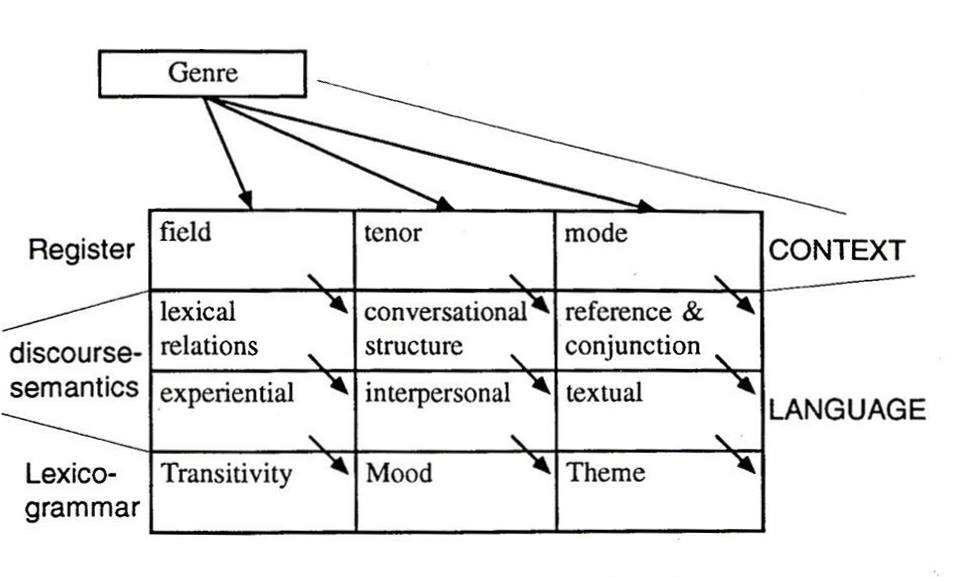
\includegraphics[width=0.85\textwidth]{../images/egginsfixed.jpg}
		\label{fig:eggins}
		\caption{Strata and metafunctions of language (from Eggins, 2004)}
		\end{figure}

		Three key factors informed our decision to adopt the SFL framework for our study. First, in contrast to most mainstream grammars, SFL conceptualises lexis and grammar as a different ends of the same system: lexis is the most delicate realisation of grammar \cite<see>{hasan_grammarians_1987}. Such a conceptualisation, we believe, is vital to an investigation of the behaviour of a concept in a large text corpus, as much of this behaviour will indeed be grammatical. Accordingly, in this study, automated parsing of corpus texts is used to carry out (often simultaneous) searches of both grammar and lexis.

		The second benefit of SFL to our research aims is that SFL is explicitly designed as a framework that to make it possible to say meaningful things about how real-world instances of language work to build meanings and perform social functions. It is thus an \emph{appliable linguistics}, built to `empower researchers to undertake projects of investigation and intervention in many contexts that are critical to the workings of communities and the quality of human life' \cite[p.~437]{matthiessen_applying_2013}.

		Finally, SFL contains the best-articulated means of systematically connecting instantiated lexicogrammatical units (i.e. wordings) to the more abstract stratum of discourse-semantics (i.e. meanings) \cite{eggins_analysing:_2004}. On the strength of this link is the whole endeavour of corpus-discourse research predicated: absent a systematic connection of these two planes of abstraction, corpus-assisted discourse studies lose much of their explanatory power, and corpus-informed discourse research becomes a contradiction in terms.

	\section{Risk words and the systemic functional grammar}

		Perhaps the most laudable achievement of SFL is the ability of its grammar (admitted even by critics, e.g. \citeNP{widdowson_text_2008}) to connect the three kinds of meanings to distinct components of lexicogrammar in consistent, stable ways. Interpersonal meanings are made through the \textbf{mood system}, including features such as \emph{modality} and \emph{modulation}. Textual meanings are made through the use of \textbf{systems of reference and conjunction} between and within clauses. Experiential meanings are made via the \textbf{transitivity system} (predicators, their subjects and object arguments, and adjuncts, in more mainstream grammars). This latter system is of most interest to us.\endnote{Though role relationships between journalists and their readership have undergone significant shifts (especially since the popularisation of online news), charting these changes falls largely outside the scope of this project.}~
		In SFL, transitivity analysis of a clause involves breaking it down into its \emph{process}, \emph{participants} and \emph{circumstances}, realised by verbal groups, nominal groups and adverbials/prepositional phrases, respectively. Most central is the process, whose head (the rightmost verb in a verbal group), may be grouped into five types: \textbf{material processes} (doing and happening: \emph{Risk declined}), \textbf{mental processes} (thinking: \emph{She thought it risky}), \textbf{verbal processes} (saying: \emph{We talked about the risks}), \textbf{existential processes} (\emph{There are risks}) and \textbf{relational processes} (being and having: \emph{It seemed risk-free}). Each type has different configurations of possible participants: mental processes have \emph{Senser} and \emph{Phenomenon} (the sensed); material processes generally have an \emph{Actor}, in subject position, with optional participants such as \emph{Goal}, \emph{Range} and \emph{Beneficiary}. Circumstances (e.g. `\emph{this week}' in Figure \ref{fig:transannotation}) provide specifications such as the manner, extent or location of the process. Circumstances are more syntactically flexible, in that they are often able to be placed in a number of positions within the clause.

			\begin{figure}[htb]
			\centering \small \onehalfspacing
    			\begin{tabularx}{0.75\textwidth}{|l|l|X|X|X|}
    			\hline
    			\emph{But}     & \emph{the bang of the gavel}             & \emph{can hold}          & \emph{risk} & \emph{for novices}          \\ \hline
    			~ & Participant: & Process: & Participant: & Circumstance:  \\
    			    			~ & Carrier & Relational \mbox{attributive} & Attribute &  Extent \\ \hline
    			\end{tabularx}
			\caption{Transitivity analysis of a clause}
			    			\label{fig:transannotation}
			\end{figure}

		An important caveat remains. SFL considers each kind of meaning as having a \emph{congruent} realisation in the lexicogrammar---participants are congruently nominal; qualities as congruently adjectival. Aside from simply using native speaker intuition tests, SFL theorists argue that congruent forms often can be identified by their \emph{typicality} and their \emph{unmarkedness}: congruent realisations are expected to be more frequent in the language as a whole, and to involve fewer derivational morphemes (\emph{nation} as a thing is less inflected than the quality, \emph{national}) (Lassen, 2003). That said, as \citeA[p.~?]{halliday_introduction_2004} explain, `it is by no means easy to decide what are metaphorical and what are congruent forms'. \emph{Risk} is in itself a good example of a concept that straddles the terrain between participant, process and quality.

		%Lassen: Imperative readings of grammatical metaphor

		Incongruent choices, however, are also common in many kinds of texts, carrying a `very considerable semantic load' \cite[p.~?]{halliday_introduction_2004}. First, through \emph{grammatical metaphor}, semantic processes may be realised grammatically as participants (`I accepted \emph{the invitation}') for the purpose of packing more information into clauses---a key feature of written journalistic text \cite{simon-vandenbergen_grammatical_2003}. Furthermore, similar meanings may be made at different ranks/strata of language: `a good risk' and `a risk is good' communicate the same positive appraisal of the same participant, but at different levels (group/phrase level via adjectival modification in the first example; clause level via relational ascription in the second). Incongruence poses serious challenges for corpus linguistic studies of discourse, as it limits our ability to locate, for example, all the ways in which risk is evaluated, graded or judged. This issue is exacerbated if, in line with SFL theory, we consider all lexicogrammatical choices to be meaningful and purposive, including the author's decision to invoke an incongruent form \cite<as in>{eggins_introduction_2004}. In some cases, rank-shifted meanings may be found using increasingly complicated lexicogrammatical search queries (see Figure \ref{fig:glossed} for an example). Automatic location of some other cases remain at this point beyond our capabilities: in appraisal at the level of clause-complex (`\emph{I see a risk---it's a big one}') extremely complex grammatical searches would be needed to first recover the identity of \emph{it} and \emph{one} as \emph{a risk}, before we could automatically determine that the risk is being semantically modified by \emph{big}. Accordingly, our analysis is limited to group/phrase and clausal levels, with meanings made via the clause complex excluded.

	\begin{table}
	  \centering
		  \begin{tabular}{|l|}
		  \hline
		  Clause complex \\ \hline
		  Clause		 \\ \hline
		  Group/phrase   \\ \hline
		  Word		   \\ \hline
		  Morpheme	   \\ \hline
		  \end{tabular}
		  \caption{Rank Scale in SFL}
		  \label{tab:rank}
	  \end{table}

		\subsection{Risk and the experiential metafunction}

			%Risk, as well as the French \emph{risque}, have a long history of use as both noun and verb \cite{hamilton_meanings_2007}, though otherwise its etymology is largely unknown. The lack of derivational morphemes makes it difficult to tell whether risk is congruently a process or a participant. Accordingly, we do not assume it to be congruently either.

			We situate our analysis of risk words predominantly within the experiential realm of meaning. At the most abstracted level of this dimension of language, we are interested in changes in the field of discourse in which risk as a concept is instantiated: \emph{has risk shifted, as per key claims of sociological theory, from international relations toward population health?} Then, within these fields, we are interested in the constellations of happenings in which risk may play a role: \emph{when risk is a process, what participants are involved? When risk is a participant, what is it a participant in, and with whom? And when risk is part of a modifier, what kind of participants and processes does it modify, and how?} Through categorisation of the kinds of fields in which risk appears, as well as the kind of participants who are positioned as riskers, risked things and potential harms, we can then empirically test the claims of influential sociological examination of risk discourse (See Table \ref{tab:claims}).


			~\ \todo[inline,color=green!40]{\noindent Either this needs to be expanded, or the mood description contracted...}
			

				%ARGUABILITY \cite[p.~271{matthiessen_combining_2002}, \cite[p.~115]{halliday_introduction_2004}.
				%PP as mini relational clause: \cite{matthiessen_lexicogrammatical_1995}

				%\cite{halliday_grammar_1996}

	\subsection{Risk and the interpersonal function: arguability}

		Though our analysis is for the most part concerned with experiential meanings (via the Transitivity system), some aspects of interpersonal meanings (via the Mood system) are also relevant. Accordingly, a brief sketch of the mood system is required.

		In SFL, the Mood system is used to give and request information (semiotic commodities) or goods and services (material commodities). Congruently, interrogatives request information, and imperatives request goods and services. Declaratives provide information. Being by far the most common mood type in news discourse, our analysis is focussed on the structure of the declarative. A declarative clause contains a Mood Block, which contains a Subject and Finite (see Figure \ref{fig:moodannotation}). Locating the constituents of the Mood Block is simple: if a tag question is added to this declarative (\emph{the bang \dots can hold risks \dots, can't it?}), the tag picks up the Subject and the Finite (with polarity reversed).

		Modality, also a component of the interpersonal metafunction, concerns modification of propositions with speaker judgements.\endnote{The corpus contained too few modalised risk predicators for analysis of longitudinal change in modalisation.}
		Prototypically, Modality is expressed through modal auxiliaries in the Finite position (\emph{I can/should/might go}). Through Modality, speakers `construe the region of uncertainty between yes and no' \cite[p.~147]{halliday_introduction_2004}. In Figure \ref{fig:moodannotation}, for example, \emph{hold} is modalised through \emph{can} in order to express the author's judgement as to the possibility of the banging of the gavel holding risks.

			\begin{figure}[htb]
			\centering \small \onehalfspacing
    			\addvbuffer[12pt 8pt]{\begin{tabularx}{0.75\textwidth}{|l|l|l|X|X|X|}
    			\hline
    			\emph{But}     & \emph{the bang of the gavel}             & \emph{can} & \emph{hold}          & \emph{risk} & \emph{for novices}          \\ \hline
    			~ 				& 		Subject     						& Finite 		& Predicator 		  & Complement & Adjunct  \\ \cline{2-6}
    			~ 				& 		 \multicolumn{2}{c|}{MOOD} 							& \multicolumn{3}{c|}{RESIDUE} \\ \hline
    			\end{tabularx}}
			\caption{Mood analysis of a clause}
			    			\label{fig:moodannotation}
			\end{figure}

		%how does this bit work: %Modalised declaratives to some extent pattern with the provision of goods and services, either via de(\emph{I can/will/shall visit you}) or speech acts, (\emph{I pronounce you husband and wife})

		At a greater level of abstraction, these Mood and Modality choices are responsible for the construction of role relationships between interactants: where interactants are of equal status (i.e. friends chatting at a cafe), similar overall frequencies in mood choices for each interactant may be observed. In a situation with interactants of less equal status, mood choice frequencies may vary more widely for the different participants: in a typical interaction between a professor and an undergraduate, only the professor is likely to use imperatives to issue commands. Importantly, as with experiential meanings, incongruence may occur, though the motivation for incongruence is an interpersonal one, such as politeness or face saving (\emph{Shut the door!/Could you shut the door?}). For us, however, this kind of incongruence does not pose the same level of challenge as experiential incongruence, as print news journalism as a genre rarely commands or requests information from the reader, and as the faces of both writer and reader are rarely under threat.

		We are interested in Mood mostly because Mood is the system through which \emph{arguability} of propositions is mediated. In SFL, arguability is used to denote the relative ease of challenging or refuting a proposition, and thus, the level of implicitness of a meaning made about the world.

		Chiefly, arguability rests in the two components in the Mood Block---the Finite and the Subject. To make a proposition arguable, it must be grounded in time and space, or to a speaker judgement of its validity. These are the two potential functions of the Finite. Locating a proposition within time and space is done through adding primary tense (\emph{lives were risked}). Meanings are linked to speaker judgements through modality (\emph{lives might be risked}) \cite[p.~116]{halliday_introduction_2004}. In either case, the Finite grounds the proposition with reference to the current exchange being undertaken by the interactants. Primary tense situates a proposition according to what is present at the time the utterance is made---it indicates `the time relative to now' \cite[p.~116]{halliday_introduction_2004}. Modality either expresses an assessment of the validity (probability, certainty, obligation, etc.) of a proposition (\emph{it might/will/must happen}) or, in an interrogative, invites the addressee to make this assessment (\emph{might/will/must it happen?}).

		The Subject is the second component of arguability. Semantically, SFL treats the Subject as `something by reference to which the proposition can be affirmed or denied' \cite[p.~117]{halliday_introduction_2004}. In the contexts of proposals and commands, it is the one who is supposed to perform the action (\emph{Shut the door, will you?}/\emph{I'll speak to her, shall I?}). In the case of declarative information provision, the Subject is the thing upon propositional validity rests. In \emph{the bang of the gavel can hold risk for novices}, for example, a refutation still requires a coherent Subject and Finite, while the Residue is only required if it is the challenged component:

\begin{quote}
\small
\begin{enumerate}	\setlength\itemsep{-0.5em}
		\item No, \emph{it should} hold risks (refuting modal finite/speaker judgement)
		\item No, but \emph{a handshake can} (refuting Subject)
		\item No, but \emph{it can} hold excitement (refuting Complement)
		\item No, but \emph{it can} for experts (refuting Complement)
\end{enumerate}
\end{quote}
		%
		Thus, the Mood Block is the most arguable part of a proposition---`it carries the burden of the clause as an interactive event' \cite[p.~118]{halliday_introduction_2004}. The steps an interlocutor needs to take to deny the validity of a meaning are fewest when the disagreement concerns the composition of the Mood Block. Meanings made within Complements and Adjuncts, or within groups or phrases, are more implicit: they support, rather than enact, meanings made within the Mood Block \cite{matthiessen_combining_2002}.

		%In this investigation, as in \citeA{matthiessen_lexicogrammatical_1995,matthiessen_combining_2002}, arguablity is also operationalised as a cline, with meanings ranging from very arguable to very inarguable based on the rank at which they are made.  Heads of processes and participants are arguable. Internal modification of groups, especially within subordinate clauses, are likely to be very inarguable. Circumstances---that is, PPs modifying the process---sit in the middle of the two extremes.

		With these descriptions, we can now operationalise arguability with regard to experiential and interpersonal metafunctions, as well as the internal structure of groups and phrases.

		\begin{table}
		\centering
		\footnotesize
   		\begin{tabular}{|l|l|l|l||l|}
		\cline{1-4}
		\multicolumn{2}{|c|}{\textbf{Metafunctions}} & \multicolumn{2}{c||}{\textbf{Lexicogrammar}} & \multicolumn{1}{c}{~} \\ \hline
   		 \emph{Experiential}  & \emph{Interpersonal}   & \emph{Rank scale}         & \emph{Group structure} & \emph{Arguability} \\ \hline
   		 Process       & Finite, Subject & Clause       & Head            & \textbf{Higher}                   \\ \hline
    		Participant(s)  & Complement      & Group/phrase & Modifier        & \textbf{Medium}                 \\ \hline
    		Circumstances & Adjunct         & Word         & Submodifier     & \textbf{Lower}                    \\ \hline
   		\end{tabular}
		\end{table}

			%\begin{table}
	  %\centering
		  %\begin{tabular}{|l|l|}
		  %\hline
		 	%\textbf{Rank scale} & \textbf{Arguability} \\ \hline
		  %%Clause complex & --- \\ \hline
		  %	Clause	 & Very arguable \\ \hline
		  %Group/phrase   & Arguable \\ \hline
		  %Word		   & Somewhat inarguable \\ \hline
		  %Morpheme	   & Very inarguable \\ \hline
		  %\end{tabular}
		  %\caption{Rank scale and arguability as operationalised here}
		  %\label{tab:rankarg}
	  %\end{table}

	  In the context of risk words, this conceptualisation of arguability can be used to empirically examine key sociological claims. Increasing prevalence of risk words generally would mean that risk words have an inbound trajectory in the NYT generally. Increasing risk words within the Mood Block would indicate that risk is discussed and argued about. A shift from Mood Block to Residue risk would indicate greater implicitness and inarguability of risk. At the same time, risk words as heads of groups/phrases would indicate greater discussion of risk, while risk words as modifiers would indicate implicitness.
		
	%\section{SFL and news discourse}

		%~\ \todo[inline,color=green!40]{\noindent Still to write ... }

			%\begin{enumerate}
			%\item Situate our research area as `hard news' \cite{gonzalez_rodriguez_tracing_2006}
			%\item Text and context in hard news
			%\item \citeNP{bednarek_evaluation_2006} % http://books.google.com.au/books?hl=en&lr=&id=8nk0BArolPwC&oi=fnd&pg=PR5&dq=%09+Evaluation+in+media+discourse+:+analysis+of+a+newspaper+corpus&ots=IFz58ZksVq&sig=gRPv0070_O31kOYTCwiBKrLC16Q&redir_esc=y#v=onepage&q=Evaluation%20in%20media%20discourse%20%3A%20analysis%20of%20a%20newspaper%20corpus&f=false
			%\item Limitations and points of difference
			%\end{enumerate}
			%}

	\section{SFL and corpus linguistics}

		Methodologically, our study may be characterised as an attempt to combine the systemic functional conceptualisation of language with practices from diachronic corpus linguistic (CL) research. As \citeA{hunston_systemic_2013} notes, SFL and CL share a number of underlying similarities, such as an emphasis on natural language a focus on register/genre as shaping the lexicogrammatical choices made in texts. More fundamentally, both CL and SFL posit that we can learn about these texts through quantification of their various lexical, grammatical and semantic properties. %Less commonly noted are that both SFL and corpus linguistics are probabalistic, and accordingly, both have predictive applications \cite{halliday_corpus_1991}.

		We use SFL and CL in tandem to locate patterns in texts without manual interpretation or categorisation. Sociological insights into key events and movements are then mapped at later stages to observed lexicogrammatical and discourse-semantic change in the behaviour of risk words (challenges in balancing the systemic-functional notion of context-in-text with the use of sociological methods are discussed below). Such an approach is characteristic of the emerging field of \emph{corpus-assisted discourse studies} (CADS). The oft-noted `methodological synergy' of CL and discourse analysis allows researchers a greater degree of empirical and quantitative support for claims, as well as a larger body of examples that can easily be accessed and qualitatively analysed \cite{baker_useful_2008}. In terms of risk, corpus-based methods allow an empirical testing of sociological literature that has tended to invent examples of clauses containing risk words, despite there being little evidence that these phrases are commonly instantiated in general language use \cite{hamilton_meanings_2007}. Research has also tended to conflate risk words with the concept of risk itself, even though the word may not be critical to the experiential meaning of a clause (the \emph{risk management team went for coffee}) and even though the latter is often present without the linguistic instantiation of the former.

		Work within CADS varies chiefly in the extent to which the corpus itself is the focus of the investigation. In \emph{corpus-driven} work, researchers are attempting to demonstrate that the corpus itself contains particular patterns of discourse. Theories are developed inductively according to patterns located in the data. \emph{Corpus-informed} studies, on the other hand, may use the corpus as a body of examples that can be drawn upon in discussion of broader trends in society \cite{baker_useful_2008}. Theories to be tested are developed before the corpus interrogation

		Our study is in the latter domain.\endnote{Though we are focussed on corpus-assisted investigation at present, indeed the dataset under investigation is of size and scope as to be of interest to corpus-driven researchers, language and media specialists, etc., and indeed, such projects are forthcoming.}
		As a diachronic investigation, we can further situate our method within \emph{Modern Diachronic CADS}. As Partington explains, 

		\begin{quote}
		\lbrack MD-CADS\rbrack~ employs relatively large corpora of a parallel structure and content from different moments of contemporary time \dots in order to track changes in modern language usage but also social, cultural and political changes as reflected in language \citeyear[p.~83]{partington_modern_2010}.
		\end{quote}

		\noindent As newspapers are well-structured and archived in digital collections, they have formed a common datasource for CADS. \citeA{johnson_`political_2003-1} investigated shifts in the discursive construction of \emph{political correctness} in German newspapers. \citeA{duguid_newspaper_2010} performed thematic categorisation of the keywords from two collections of digitised newspapers from 1995 and 2005. \citeA{freake_cross-linguistic_2012} focussed on the ideological positioning of French and English in Canadian newspapers. %do these consider current events??

		Ours is not the first corpus-based study of risk. Most well-known is \citeA{fillmore_toward_1992}, who studied the behaviour of risk as both noun and verb in a 25 million word corpus of American English. Ultimately, the authors' aims were lexicographic, rather than discourse-analytic, limiting the usefulness of the study's methods for our purposes. A second key point of difference is the small size and lack of structure of their corpus (though their research was a certainly remarkable and groundbreaking effort at the time of publication). Finally, their study was neither longitudinal, nor designed to connect patterns to social/societal change.

		More recently, \citeA{hamilton_meanings_2007} used a frame semantics approach to understand the behaviour of risk in two corpora: the 56 million word \emph{Collins WordbanksOnline Corpus} (N risk tokens) and the five million word \emph{CANCODE} (235 risk tokens). 
		%Frame semantics is a well-established framework for functional analysis of language. 
		We depart from their methods in five respects. First, they use general corpora, while we used a specialised corpus. Second, our study is diachronic, while theirs is largely monochronic. Third, we differ dramatically in the number of risk words analysed (n/n). Fourth, they relied on collocation (without lemmatisation\endnote{Lemmatisation is the process of counting the base forms of tokens, rather than the token itself. \emph{Taken} would be classified under \emph{take}, for example. While lemmatisation is not \emph{always} the best option, as it can collapse different parts of speech, tense information, etc., it is certainly appropriate when determining the most common predicators, etc.}), while we performed specific queries of the lexicogrammar, using lemmatisation where needed. Sixth, they used frame semantics, while we use SFL (though informed by Filmore and Atkins' \citeyear{fillmore_toward_1992} articulation of the components of the risk frame). Though these theories have a number of underlying similarities (both are semantically oriented grammars, for example), the two diverge in their treatment of the role of cognition and psychology. While frame semantics argues that lexicogrammatical instantiations are mapped by listeners to preexisting cognitive frames or schemata, SFL is largely silent on the subject of cognition, preferring to map lexicogrammar to external variables of field, tenor and mode.

		%frame semantics vs sfl: http://ucrel.lancs.ac.uk/publications/cl2003/papers/hunston.pdf
		
		%They relied on manual thematic categorisation of concordance lines---something not practical for a corpus containing as many tokens as ours. Their reliance on collocation meant that lists of the closest collocates of risk are not organised by part of speech. This makes it hard to draw meaningful conclusions. Results are also not lemmatised---\emph{is} and \emph{are} are both listed as lower-significance collocates, though had they been classed together with all forms of \emph{be}, \emph{be} may have been demonstrated to play a more important role. Also, their corpus is `balanced', while ours is from a single source.

		Notably, our methodology also departs from typical methods of (MD-)CADS in a few key respects. First, CADS is often lexically-oriented, with techniques such as \textbf{keywording} used as a means of disinterring the `aboutness of a text' \cite{baker_querying_2004} and \textbf{clustering} and \textbf{collocation} used to look for the co-occurrence of lexical items absent any consideration of grammar. \citeA{hunston_systemic_2013} contends that despite a number of areas of overlap, SFL and CL are at odds in the sense that SFL is grammatically oriented while CL is lexically oriented. Though the majority of CADS does indeed focus on lexis, this preoccupation stems more from the relative simplicity of searching for tokens in corpora, compared to grammatical features, than it does from any theoretical motivation.\endnote{We need only to look at the number of lines of code needed to develop an accurate tokeniser and an accurate grammatical structure parser to understand the reasons why lexis appears as the de-facto centre of CL/CADS today}~Accordingly, our use of grammatically parsed data and equal consideration of lexical and grammatical features, though in line with SFL, is against the grain of much contemporary CADS literature.

		The second key difference from mainstream CADS is that we did not rely on typical practices such as keywording, clustering, collocation and the use of stopword lists. Our reasons for avoiding these practices are varied. Keywording we found to be problematic due to its reliance on a reference corpus of general language. The usefulness of this reference corpus is predicated on the idea of corpus balance---that is, the notion that a corpus of texts, if comprised of a wide variety of genres, and if the relative proportion of these texts is akin to their prevalence in culture, may be taken to be representative of language generally \cite{chen_sinica_1996}. As corpus balance is well-acknowledged by CADS practitioners to be only a theoretical ideal (Gries, 2009), we took a different approach. Rather than keywording, we simply counted the base forms of the most common heads of participants, processes and circumstances in each subcorpus. This also liberated us from the arbitrary nature of stopword lists (lists of very common words that are automatically excluded from search results), as most stopwords are determiners, prepositions, conjunctions and so on, which rarely occupy key experiential roles.

		Clustering and collocation, though mainstays of CADS, are also absent in our analysis, as they consider only the co-occurrence of lexical items within a specified (and arbitrary) number of words, and accordingly do not take grammatical relationships into account. As an example, \emph{Men are from Mars, and women are from Venus} would contribute to an understanding of \emph{Mars} and \emph{women} as collocates, regardless of the fact that the experiential meaning of the clause has the opposite meaning. We instead created nuanced search queries capable of drawing on lemma lists and lists of process types (as in Figure \ref{fig:glossed}). This luxury was afforded by grammatical (phrase structure and dependency) annotation of the corpus, as well as the development of scripts for quickly searching lexicogrammar.

		%Quantitative corpus linguistics with R: a practical introduction

		%This was primarily to avoid conflicts between these practices and the theoretical orientation discourse analysis:

			\begin{figure}
			\begin{quote}
			\begin{multicols}{2}
			\begin{verbatim}
			__ >># (/(NP|VP|PP)/ > (VP
			<<# "RelationalProcess" $ 
			(@NP <<# /(?i)man/)))
			\end{verbatim}
			\noindent In relational processes in which \emph{man/men} is the Token/Carrier, what is the head of the Value/Attribute?
			\end{multicols}
			\end{quote}
			\caption{\emph{Tregex}-based search query and gloss}
			\label{fig:glossed}
			\end{figure}

			\section{Discourse-semantic areas of interest}

				Our interest is ultimately in discourse-semantic experiential and interpersonal meanings of risk words. The first point of interest is simply the relative frequency of risk words in the NYT generally, and by word class. These areas of interest are at the clausal level. Within experiential meaning, we are interested the relative frequency of risk as a Participant and as a Process, as well as the behaviour of risk when occupying these roles. At the same time, we are interested in meanings made below clause level, within groups and phrases. When risk is a participant or process, we are interested in the ways it is modified. Furthermore, risk itself can be a modifier of participants and processes. Accordingly, we are also interested in both understanding the ways in which this modification happen and finding the participants and processes that risk commonly modifies. Finally, within the interpersonal realm of meaning, we are interested in the arguability of risk words---that is, the extent to which their meaning is symbolically available to negotiation by the writer/reader.

				We can summarise our discourse-semantic interests with the following \ref{lst:num} questions. \emph{In terms of longitudinal change in the NYT,}

				\begin{enumerate}\setlength\itemsep{-0.5em}
					\item \emph{How frequently do risk words appear?}
					\item \emph{Which experiential roles do risk words occupy?}
					\item \emph{Is risk more commonly in the position of experiential subject or experiential object?}
					\item \emph{What processes are involved when risk is a participant?}
					\item \emph{How are participant risks modified?}
					\item \emph{What kinds of risk processes are there, and what are their relative frequencies?}
					\item \emph{When risk is a process, what participants are involved?}
					\item \emph{When risk is a modifier, what are the most common forms?}
					\item \emph{When risk is a modifier, what is being modified?}
					\item \emph{How arguable is risk?} \label{lst:num}
				\end{enumerate}
				%
				These questions are answered in this order in the Findings section. In the Discussion, these answers are synergised in order to perform a broader analysis of discouse-semantic change.

		\section{Lexicogrammatical realisations of discourse-semantic meanings}

			Discourse-semantic meanings are realised in texts by lexicogrammatical patterns. \textbf{Risk as participant} is congruently realised by a risk word at the head of a noun phrase that is an argument of a main verb. Other possible realisations of risk participants are adjectival risk words in participant positions (\emph{The job is risky}) or risk words within prepositional phrases (\emph{Votes were at risk}). SFL also treats prepositional phrases as partially realised relational processes, containing only object arguments. As this is perhaps a controversial analysis within linguistic theory generally, the treatment of risk within PPs is separated from risk as arguments of verbal groups. \textbf{Risk as a process} is congruently realised by a risk word as the main verb of a clause. When risk is instantiated here, we can extract the participants involved in the process. \textbf{Risk as a modifier} is realised by different word classes, depending on what is being modified. Risk can modify participants through pre-head or post-head modification. Analysed in this study\endnote{Modification through embedded clauses (\emph{the children who were at risk}) has been left out for reasons of scope.} are adjectival pre-head modification (\emph{a risky move}), nominal pre-head modification (\emph{risk management}) and post-head modification via a prepositional phrase (\emph{the electorate at risk}). \textbf{Arguability of risk words} can be determined by looking for the functional role of risk words within the Mood system: risk as Subject or Predicator is more arguable than risk as Complement and Adjunct. 

			%Risk can modify either participants or processes. Participants are modifier through pre- or post-head attachments within the nominal group (\emph{a risky decision}; \emph{a man at risk of harm}. Processes are modified by adverbials or by prepositional phrases that attach to the verbal group (\emph{he gambled riskily}; \emph{she told me about the risk}).

			%Risk as a modifier of participant. The first, most congruently, involves the use of risk as an Epithet within an adjectival unit  (e.g. \emph{the risky decision}). Note that this may serve either experiential or interpersonal functions: experiential Epithets are objective properties of the head of the phrase; interpersonal Epithets convey speaker judgements. Also possible is risk as a Classifier nominal classifiers (e.g. \emph{risk management}). Here, the head of the noun is restricted to the provided class. 

			%We can now add lexicogrammatical realisations to our discourse-semantic areas of interest:

				%\begin{enumerate}
					%\item how frequently do risk words appear?
					%\item which functional roles (Participant, Process, Modifier) do risk words occupy?
					%\item Is risk more commonly in the position of experiential subject or experiential object?
					%\item what processes are involved when risk is a subject%\slash object participant?
					%\item when risk is a process, what participants are involved?
					%\item how arguable is risk?
					%\item when risk is a modifier, what are the most common forms?
					%\item when risk is a modifier, what is being modified?
				%\end{enumerate}

			%Risk words may be nominal (\emph{a risk}), verbal (\emph{she risks}), adjectival (\emph{a risky venture}) or, rarely, adverbial (\emph{I riskily decided}).


			%Corpus interrogation proceeded through each of these four categories in a wide array of permutations. In each interrogation, we were interested in either a) counting the total occurrences of a lexicogrammatical pattern in each subcorpus (e.g. \emph{How often is a risk word adjectival?}) or b) listing all words matching a search query by total frequency in each subcorpus (e.g. \emph{Which risk-adjectives occur, and how often?}).

			%\begin{enumerate}[nolistsep]
				%\item Counting the total occurrences of a lexicogrammatical pattern in each subcorpus (e.g. \emph{How often is a risk word adjectival?})
				%\item Listing all words matching a search query by total frequency in each subcorpus (e.g. \emph{Which risk-adjectives occur, and how often?})
			%\end{enumerate}

			The scope of our project necessitated some constraints on the kinds of patterns we analysed. Major constraints included our focussing on experiential meaning, perhaps at the expense of interpersonal meaning. Thus, the analysis contains little consideration of how risk may be operationalised in order to construct writer/reader or newspaper/readership relationships. Also largely unanalysed are the ways in which risk are appraised, judged, and graded in severity. This was mostly due to the lack of available automatic parsers for SFL's appraisal grammar \cite<see>{martin_language_2005}. Finally, queries returning less salient or ambiguous results are omitted from discussion here. Counting the kinds of determiners that occur before a nominal risk (this risk, a risk, the risk) uncovered no particularly interesting patterns, for example.

				%make all queries and results available?

				%MUST CHANGE THESE PARAGRAPHS TO RISK AS PARTICIPANT, PROCESS,


		%\subsection{Dependency querying}

			%\begin{figure}[htb!]
			%\centering
			%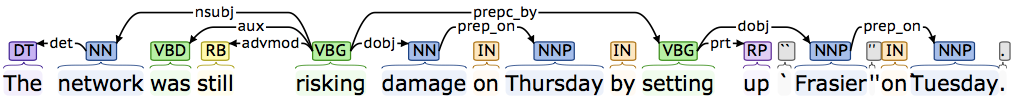
\includegraphics[width=0.75\textwidth]{../images/depparse}
			%\caption{A visualised dependency parse, with \emph{risking} as root}
			%\label{fig:depparse}
			%\end{figure}		

			\section{Operationalising sociological claims}

			The discourse-semantic and lexicogrammatical areas of interest can be summarised with regard to related sociological claims.

				\begin{table}
				\centering
				\footnotesize
				\begin{tabularx}{1.0\textwidth}{|l|X|X|X|X|}
				\hline
				\textbf{Author}   & \textbf{Claim}   & \textbf{Discourse-semantic realisations(s)}      & \textbf{Congruent lexicogrammatical realisation(s)}    & \textbf{Example(s)}  \\ \hline
				Beck     & Everyday life world characterised by risk    & Common people as increasingly common participants in risk as a process; increasingly localised risked things/potential harms; risk appearing in articles about daily life & Women, children, non-celebrities appearing as heads of nominal groups that are actors in risk processes; Everyday processes and common things appearing as head of verbal and nominal groups that appear after risk processes & \emph{The little girl risked tearing her coat}; \emph{We risked getting rained on/one dollar}; \\ \hline
				Giddens  & ~ & ~    & ~       & ~       \\ \hline
				Zinn     & ~     & ~      & ~       & ~    \\ \hline
				Author x & Increasing focus on risk in health discourse & Medical lexis (diseases, institutions, medications, etc) as increasingly common participants in risk as a process                                                         & Illnesses and risk in nominal compound words; health terminology in modifiers of risk as head of a participant    & \emph{The cancer-risk}; \emph{the risk of heart disease}                                       \\ \hline
				Author y & ~     & ~       & ~       & ~      \\ \hline
				\end{tabularx}
				\caption{Systemic-functional realisations of sociological claims concerning risk discourse}
				\label{tab:claims}
				\end{table}

			%\subsubsection{Longitudinal trajectory} will be used to refer to a given lexicogrammatical construction increasing in frequency (\emph{inbound trajectory}), becoming less frequent (\emph{outbound trajectory}), or remaining at a similar frequency (\emph{static trajectory}) over time.


%\bibliography{../references/libwin} % Methodology

%!TEX root = ../risk_report.tex

\chapter{Findings} \label{chap:findings}

    Findings are organised according to the formulation of areas of interest as questions. These questions progress from general frequency counting (Q1), through experiential meanings (Qs 2--7), to risk as modifier (Qs 8 \& 9) and finally to arguability (Q10). Discussion of the general significance of individual findings is also presented in this section, as the Discussion section synergises all findings to explain the discourse-semantics of risk.

    \vspace{5mm}
    \noindent\begin{tcolorbox}[colback=yellow!5,colframe=yellow!40!black,title=Summary: an example]
    \parbox{1\textwidth}{%
    Summaries of each major finding will be presented in highlighted text boxes.}
    \end{tcolorbox}
    \vspace{5mm}

    \noindent An \emph{IPython Notebook} interface for navigating the corpus \cite<see>{mckinney_python_2012}, as well as the code used to interrogate it and the findings we produced, is available online: \url{https://github.com/interrogator/risk}. A non-interactive version is available at \url{http://nbviewer.ipython.org/github/interrogator/risk/blob/master/risk.ipynb}. This Notebook does not suffer from spatial limitations, and thus contains additional information, including the exact Tregex queries used in interrogations, as well as complete lists of the concordance lines discussed only briefly here. Tools and results from other kinds of corpus linguistic analysis, such as keywording and collocation, are also available there, but have not been described here.

\section{How frequently do risk words appear?} \FloatBarrier

    %We successfully located a number of lexicogrammatical sites of change within clauses containing a risk word. 

    The first point of interest was the overall frequency of risk words in the NYT (Figure \ref{fig:relative_frequency_of_risk_words}) and the distribution of risk words by word class (nominal, verbal, adjectival\slash adverbial), absent any consideration of surrounding grammar (see Figure \ref{fig:wordclasses}). In terms of the relative frequency of risk words, we note a general upward trend, with a number of peaks and troughs worthy of further investigation. In terms of word classes of risk, we found that not only are nominal forms by far the most common in the NYT, but that it is nominal risk words that vary the most in frequency, with the other categories remaining more or less stable. Interestingly, in the span for which we have no data (1964--1986), adjectival forms overtake verbal forms of risk in frequency.

    %Using our reference corpus, we checked to see whether nominals were becoming more frequent within the NYT more generally.

    \noindent
    \begin{figure}[htb!]
    \centering
    \begin{minipage}{.45\textwidth}
    \centering
    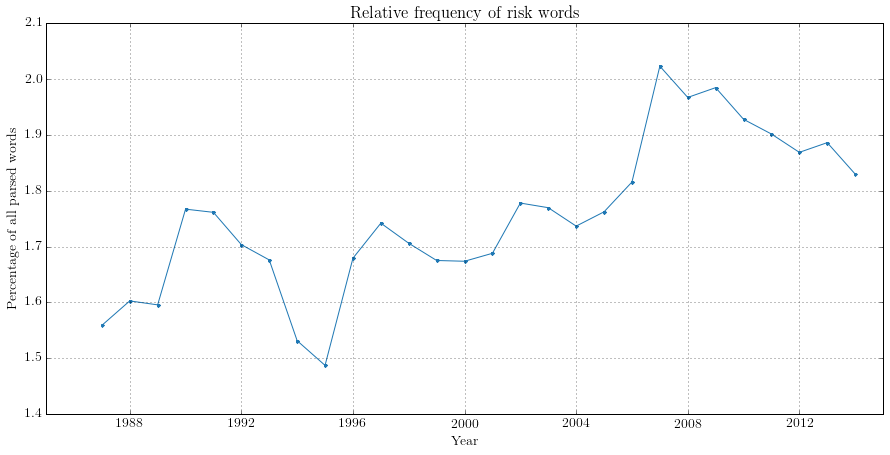
\includegraphics[width=.95\textwidth]{../images/relative_frequency_of_risk_words.png}
    \caption{Relative frequency of risk words}
    \label{fig:relative_frequency_of_risk_words}
    \end{minipage}%
    \begin{minipage}{.55\textwidth}
    \centering
    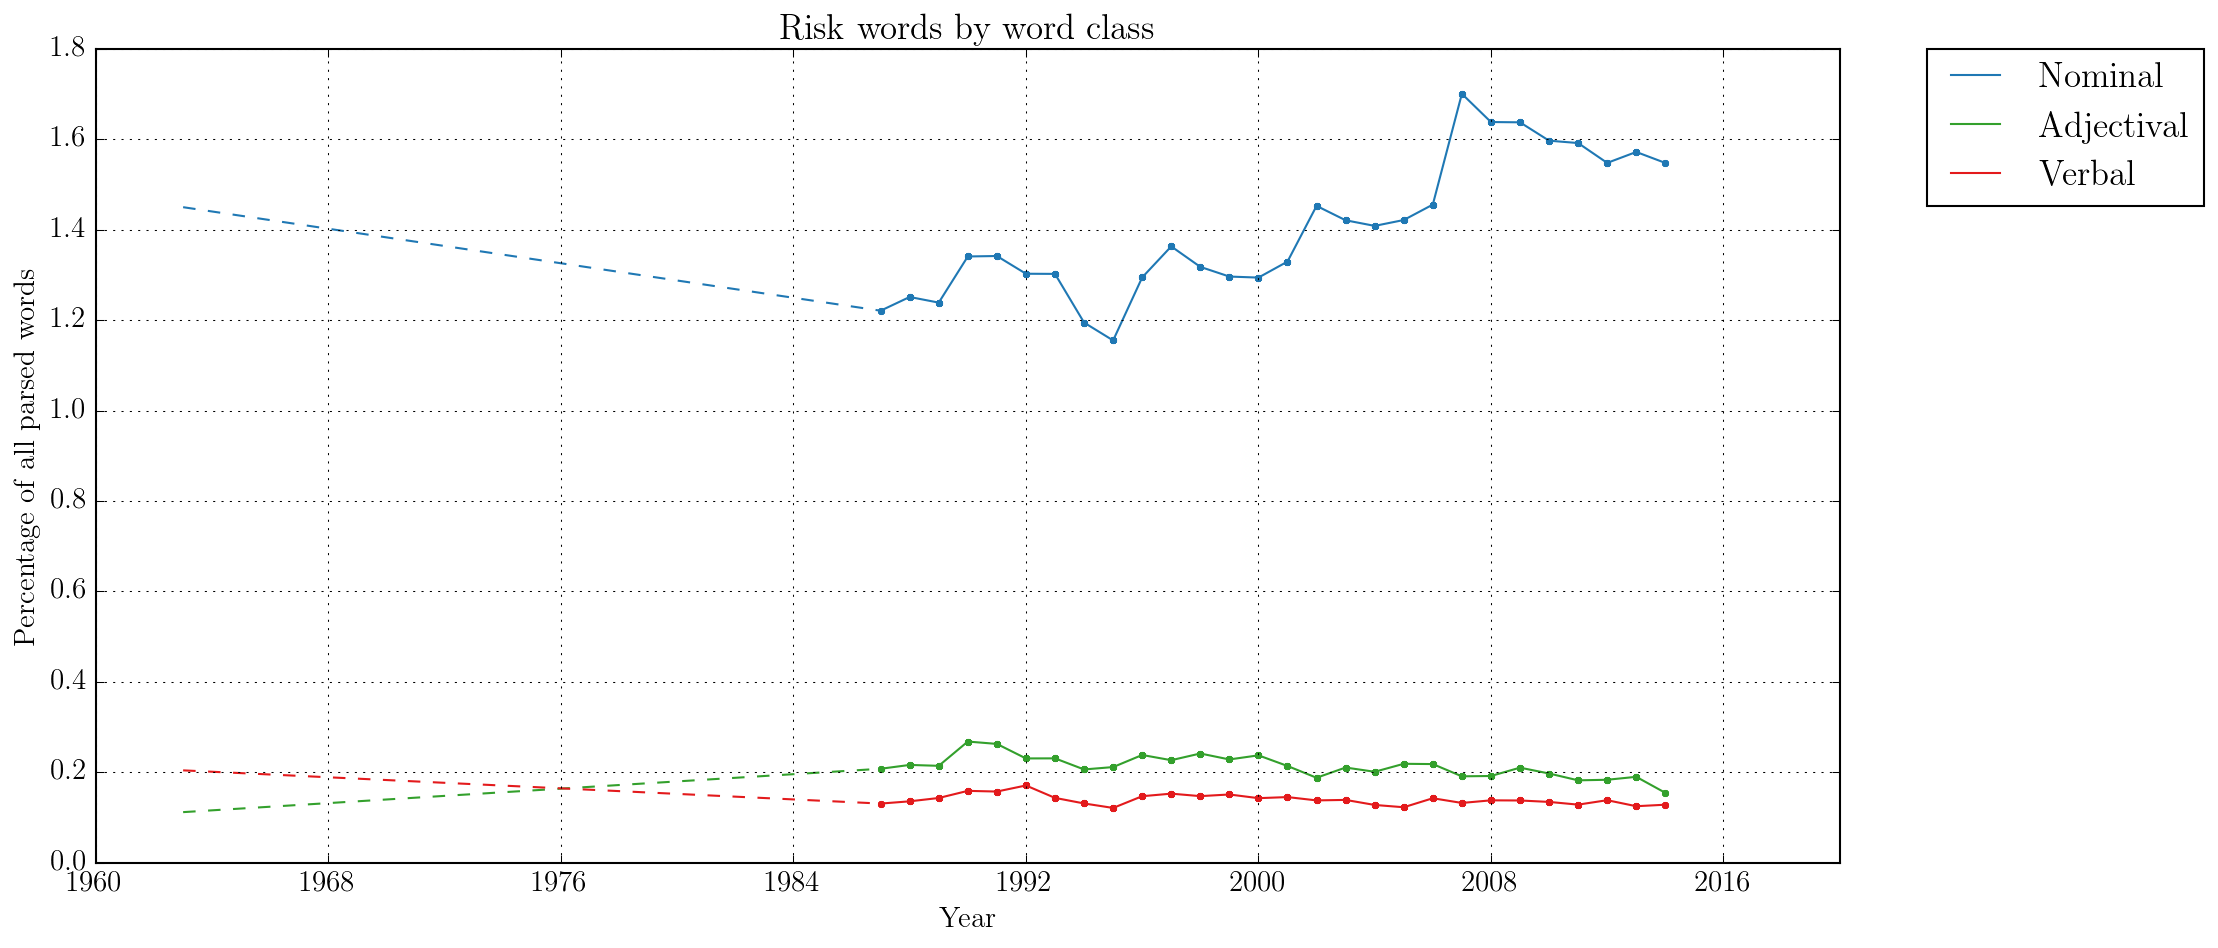
\includegraphics[width=.95\textwidth]{../images/risk_words_by_word_class.png}
    \caption{Relative frequency by word class}
    \label{fig:wordclasses}
    \end{minipage}
    \end{figure}

    %\begin{figure}[htb!]
    %\centering
    %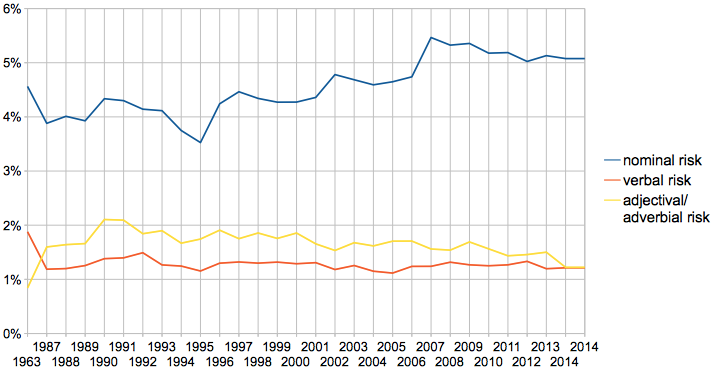
\includegraphics[width=0.75\textwidth]{../images/relwordclass.png}
    %\caption{Risk words by word class as percentage of all parsed words}
    %\label{fig:relwordclass}
    %\end{figure}

    %FUNCTIONAL CATEGORISATION?

    We compared this against the relative frequencies of nominal, verbal and adjectival\slash adverbial lexical items in the corpus as a whole, in order to account for any trends toward nominalisation in our dataset more generally (Figure \ref{fig:wordclasses}). This showed that even when compared to potential trends toward nominalisation generally, nominal risks are still on an inbound trajectory.

    These initial findings guided the rest of the investigation: particular attention was paid to nominal risks, as these were the site of the most longitudinal change. That said, these categories provide merely a categorisation of the formal features of risk words. Functionally, things are substantially more complicated: \emph{running a risk}, for example, while featuring a nominal risk, is in reality a risk process; similarly, though risk is nominal in \emph{risk management}, risk is nominal, it functions as a modifier, rather than a participant.

    A similar question is the number of unique risk words appearing per year. Figure \ref{fig:diffriskwords} demonstrates that there does appear to be a general increase in the relative number of risk words over time.\endnote{1963 is excluded from analysis here, as poor quality OCR created a number of non-word results such as \emph{risks-wnrk}, \emph{risks.North} and \emph{risks.With}.}

    \begin{figure}[htb!]
    \centering
    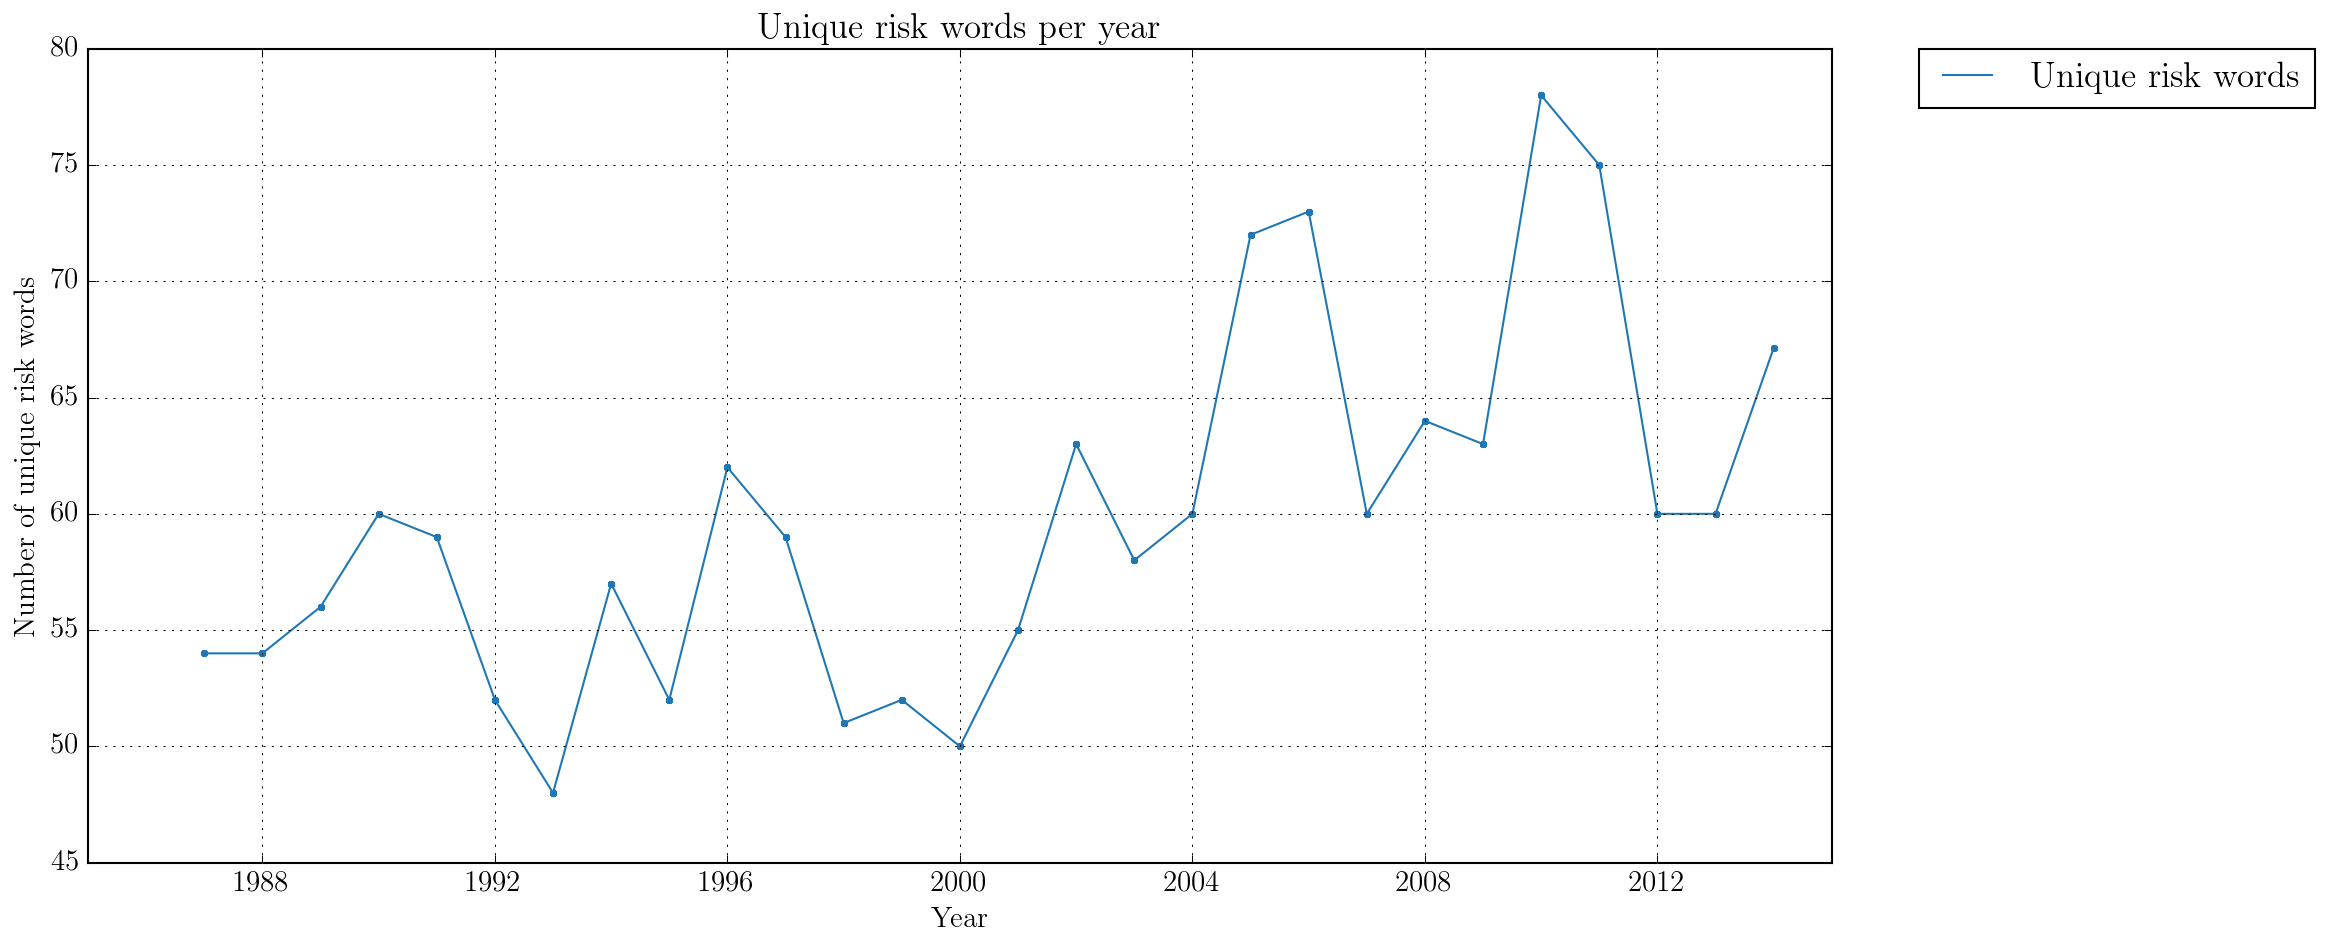
\includegraphics[width=0.7\textwidth]{../images/unique_risk_words_per_year.png}
    \caption{Unique risk words}
    \label{fig:diffriskwords}
    \end{figure}

    \vspace{5mm}\noindent\begin{tcolorbox}[colback=yellow!5,colframe=yellow!40!black,title=Summary: frequency of risk words]
    \parbox{1\textwidth}{%
    Risk words appear to be increasing in relative frequency, with modest increases in the number of unique risk words per year.}
    \end{tcolorbox}
    \vspace{5mm}



\section{Which experiential roles do risk words occupy?} \FloatBarrier

    In a systemic-functional conceptualisation of the experiential metafunction of language, risk words may take the form of a Participant (\emph{The risk was there}), Process (\emph{I risked it}) or a Modifier (\emph{a risky encounter}). Though these pattern to some extent with word classes (e.g. \emph{participant = noun, process = verb, modifier = adjective}), word classes on the whole are a poor indication of functional role, especially in genres such as print news journalism,  which rely heavily on nominalisation and grammatical metaphor to pack large amounts of experiential information into each clause. As shown in Table \ref{tab:class_and_role}, for example, nominal risks commonly perform Modifier functions, and adjectival functions often perform Participant functions.

    \begin{table}
    \small
    \centering
    \begin{tabular}{|l|l|l|}
    \hline
    \textbf{Example}       & \textbf{Word class}     & \textbf{Experiential role}     \\ \hline
    It was risky  & Adjective  &  Participant   \\ \hline
    There was a risking & Noun  &  Nominalised process   \\ \hline
    Risk management  & Noun & Modifier   \\ \hline
    \end{tabular}
    \caption{Key differences between word class and experiential role}
    \label{tab:class_and_role}
    \end{table}

    Using Stanford CoreNLP's dependency parses, we counted the frequency of risk words within these three functional roles (Figure \ref{fig:funcrole}). In line with the results from word-class based searching, we find that risk as a Process is declining in use. Risk as Modifier, patterning in part with adjectival risk, appears to be increasing. That said, we can also see here the affordances of a functional grammar in corpus assisted discourse research: in this case, much richer evidence of changing usage of risk can be found through an understanding of its semantic function rather than its word class alone.

    % today comprises a larger proportion of risk Participants than in earlier samples. 

    There is a clear trend toward using risk as a Participant.
    Nominalisation of risk is in and of itself evidence of a greater implicitness of risk, as the core function of nominalisation is to pack more information into the clause. Nominalisation thus reflects 


    In terms of experiential meaning

    Nominalisation is also closely tied to arguability. This link is discussed in Section \ref{sect:arguability}.

    %``From studies comparing identical and fraternal twins, it is estimated that genetic factors account for 40 to 60 percent of the variation in the risk for addiction.''

    %That was just one day after Richard S. Fuld Jr. , Lehman 's chief executive , announced a new strategy that he said would `` accomplish a significant de-risking of our balance sheet , '' in part by putting risky assets into a new company it would spin off to shareholders next year .

    % `` Ambac has consistently emphasized that in this period of extreme uncertainty in the capital markets , the de-risking and de-leveraging of our balance sheet is our highest priority , '' David W. Wallis , the chief executive , said in a news release .

    \begin{figure}[htb!]
    \centering
    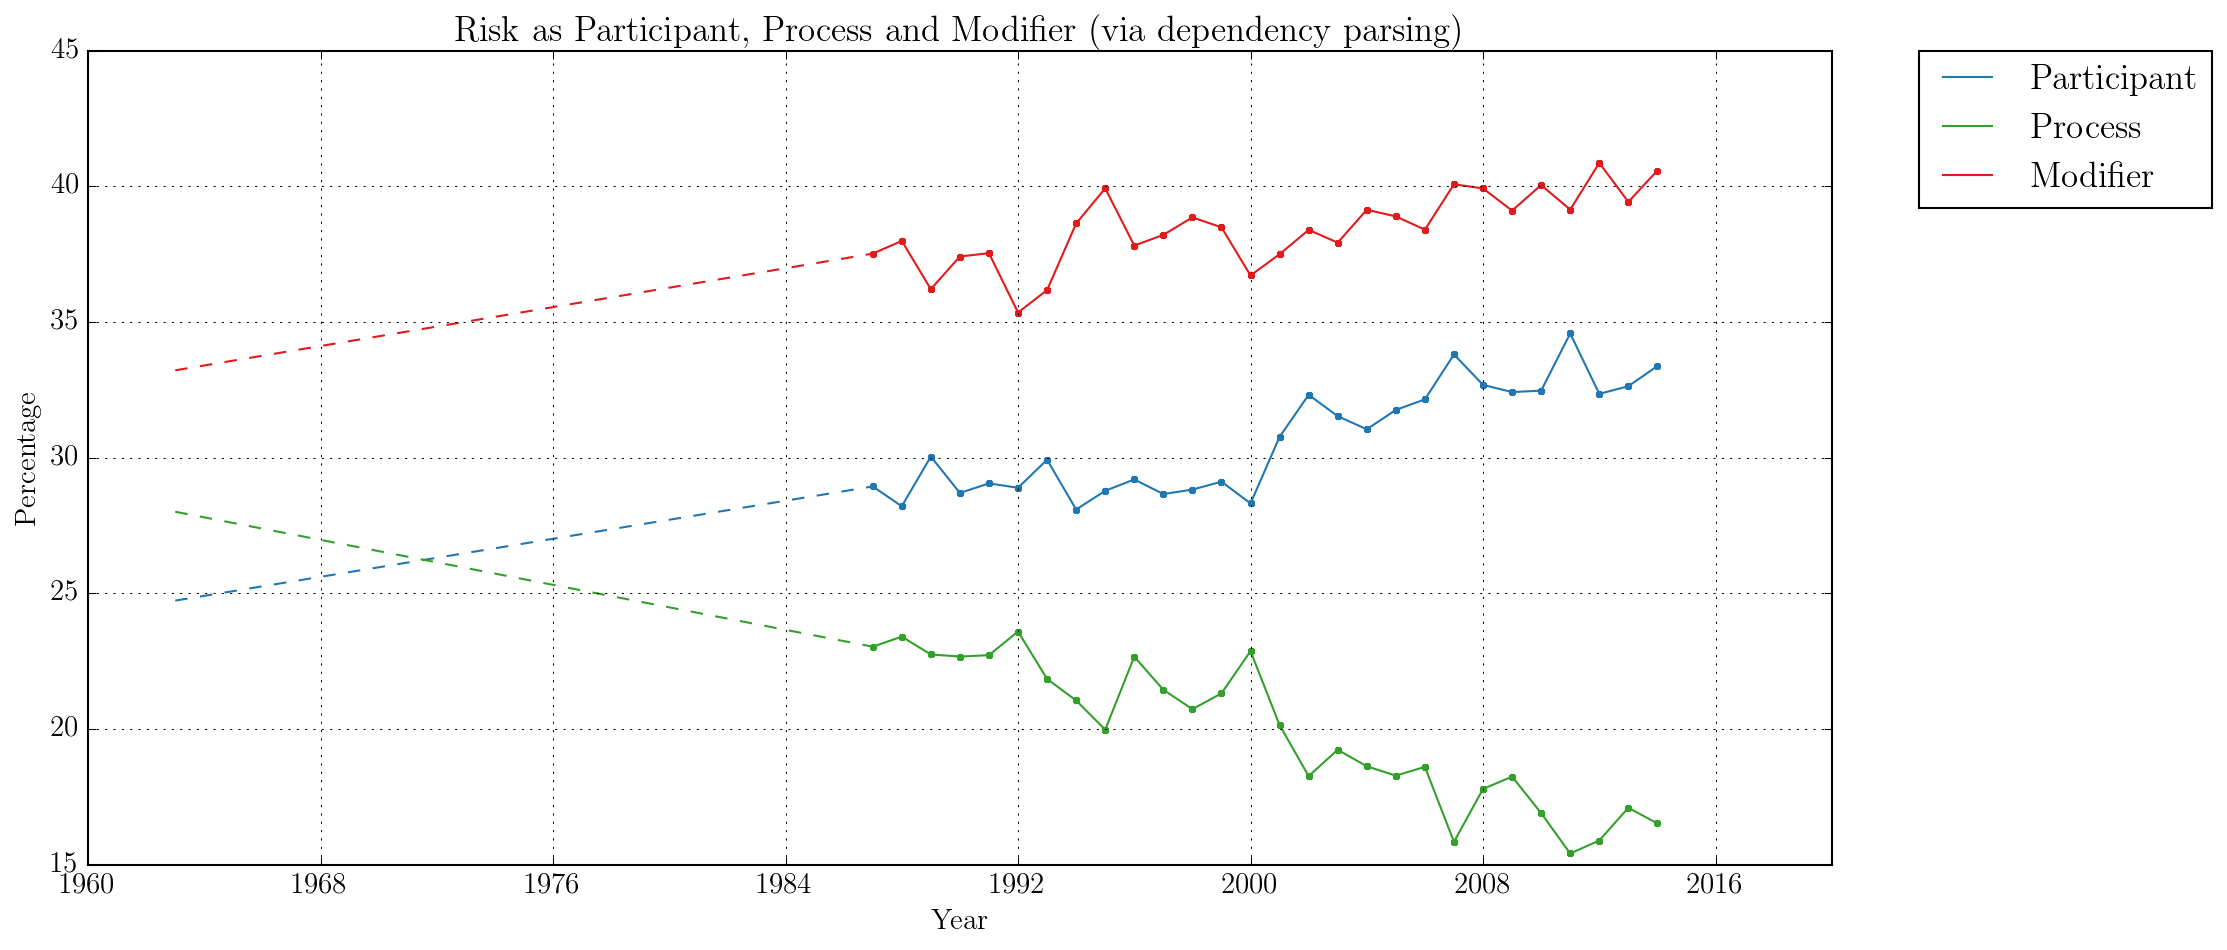
\includegraphics[width=0.7\textwidth]{../images/risk-as-participant-process-and-modifier-via-dependency-parsing.png}
    \caption{Experiential roles of risk words}
    \label{fig:funcrole}
    \end{figure}

    %~\ \todo[inline,color=yellow!40]{\noindent More discussion here, perhaps, as well as the above chart as relative frequencies. I may also have to account for risk within prepositional phrases here.}
    
    %only when the risk word forms the head of these groups, rather than a dependent/modifier (e.g. \emph{a risky decision}).

    \vspace{5mm}\noindent\begin{tcolorbox}[colback=yellow!5,colframe=yellow!40!black,title=Summary: experiential function of risk words]
    \parbox{1\textwidth}{%
    Risk as a process is declining in use, and has been overtaken in frequency by risk as a participant.}
    \end{tcolorbox}
    \vspace{5mm}

\section{Is risk more commonly in the position of experiential subject or experiential object?} \FloatBarrier

    Risk as a participant may take the form of an experiential subject or an experiential object. Our first area of interest was the proportion of each, with respect to general trends in the NYT. As shown in Figure \ref{fig:bestexpsubjobj}, risk is more commonly an object than a subject. It is also apparent that risk as experiential subject is on an static trajectory, while risk as experiential object is inbound. The significance of this is discussed in more depth in Section \ref{sect:arguability}.

    \begin{figure}[htb!]
    \centering
    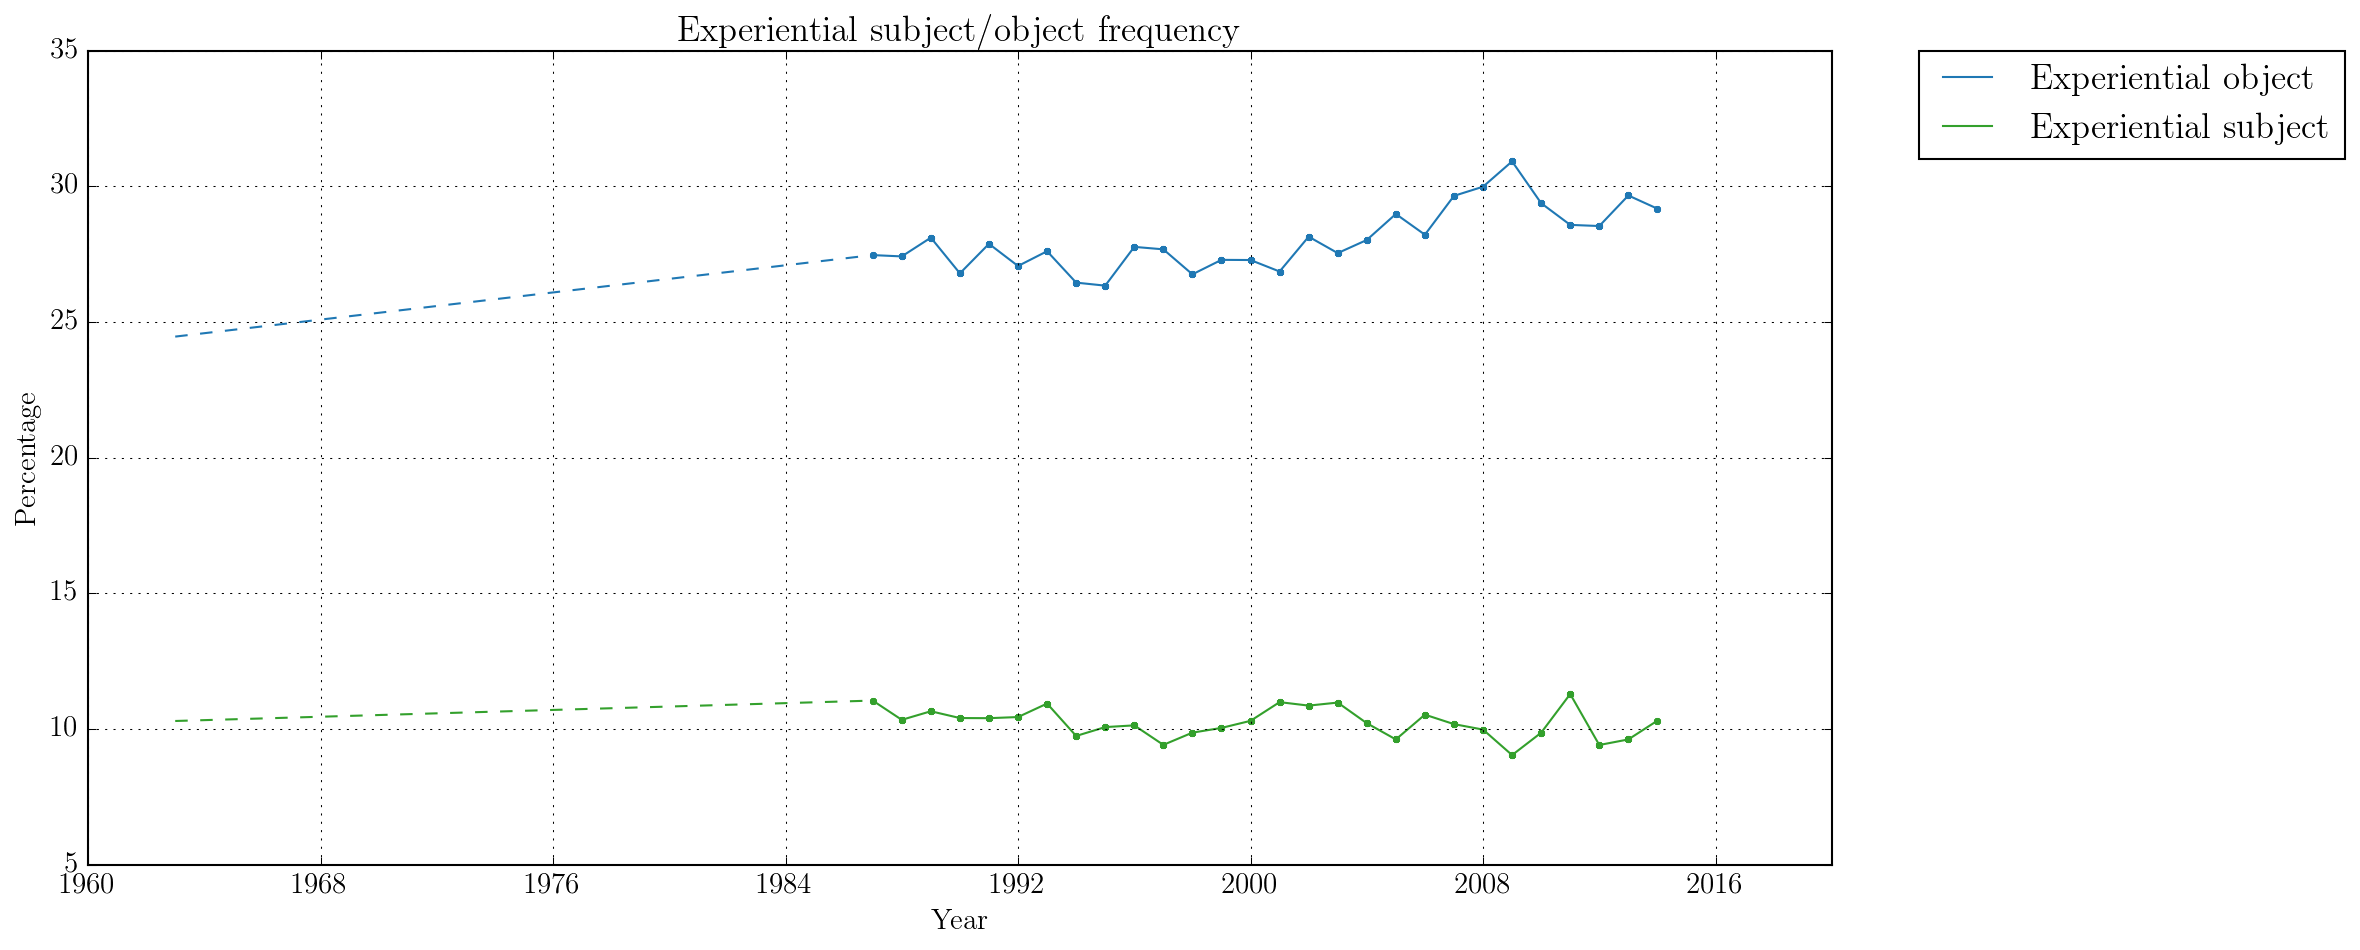
\includegraphics[width=0.75\textwidth]{../images/experiential_subject_object_frequency.png}
    \caption{Risk as experiential subject and object as percentage of all risk roles}
    \label{fig:bestexpsubjobj}
    \end{figure}
    %

    \begin{table}[tb]\footnotesize
    \centering
    \addvbuffer[12pt 8pt]{\begin{tabularx}{0.75\textwidth}{|X|X|}
    \hline
    \textbf{As subject} & \textbf{As object} \\ \hline
    \textit{But the most prevalent \textbf{risk} for the average traveler to Peru is the high altitude of the Andes}   & \textit{The company has resolved accounting problems, he said, and stabilized profit margins, while new management has reduced the company's \textbf{risks}}  \\ \hline
    \textit{The \textbf{risk} would be that the stock would recover during the period that the investor was out of the stock}   & \textit{But an empty village is a big \textbf{risk}.}  \\ \hline
    \textit{But the \textbf{risk}, though very small, that a man facing execution could win a new trial raises the question why this rule has proved so hard to follow}   & \textit{They said there was only a little \textbf{risk}, and now he 's not with us anymore} \\ \hline
    \end{tabularx}}
    \caption{Examples of risk as experiential subject and object in 2001}
    \label{tab:subj_conc}
    \end{table}



    \vspace{5mm}\noindent\begin{tcolorbox}[colback=yellow!5,colframe=yellow!40!black,title=Summary: risk as experiential subject\slash object]
    \parbox{1\textwidth}{%
    Risk is more often an experiential object than an experiential subject. The gap has widened considerably over time.}
    \end{tcolorbox}
    \vspace{5mm}



\section{What processes are involved when risk is a participant?} \FloatBarrier

    We then wanted to determine the most common processes in which risk as a participant is involved. Tables \ref{tab:subj} and \ref{tab:obj} show the top twenty processes for risk as experiential subject and object, taking passivisation into account.\endnote{\emph{Take} and \emph{run} are removed from the object column here, as \emph{take risk} and \emph{run risk} are considered risk processes.}~

    % this below doesn't count agent as an experiential subject, and it should! also copula

    \begin{table}[htb!]
    \centering
    \addvbuffer[12pt 8pt]{\begin{minipage}{.35\textwidth}
    \small
    \begin{tabularx}{1.0\textwidth}{|>{\raggedright}X|l|}
    \hline
    \textbf{Processes when risk is experiential subject} & \textbf{Total} \\ \hline
    be                                      & 8954  \\ \hline
    increase                                & 460   \\ \hline
    outweigh                                & 278   \\ \hline
    rise                                    & 269   \\ \hline
    say                                     & 222   \\ \hline
    come                                    & 201   \\ \hline
    remain                                  & 192   \\ \hline
    go                                      & 190   \\ \hline
    have                                    & 179   \\ \hline
    make                                    & 148   \\ \hline
    seem                                    & 148   \\ \hline
    involve                                 & 145   \\ \hline
    grow                                    & 133   \\ \hline
    exist                                   & 127   \\ \hline
    take                                    & 121   \\ \hline
    become                                  & 120   \\ \hline
    lose                                    & 120   \\ \hline
    include                                 & 113   \\ \hline
    appear                                  & 111   \\ \hline
    pay                                  & 100   \\ \hline
    \end{tabularx}
    \caption{Processes when risk is \mbox{experiential} subject}
    \label{tab:subj}
    \end{minipage}} \hspace{1cm} % This must go next to `\end{minipage}`
    \addvbuffer[12pt 8pt]{\begin{minipage}{.35\textwidth}
    \small
    \begin{tabularx}{1.0\textwidth}{|>{\raggedright}X|l|}
    \hline
    \textbf{Processes when risk is experiential object} & \textbf{Total} \\ \hline
    %take                                             & 11459 \\ \hline
    reduce                                           & 5609  \\ \hline
    pose                                             & 4179  \\ \hline
    increase                                         & 4063  \\ \hline
    %run                                              & 3506  \\ \hline
    have                                             & 2879  \\ \hline
    carry                                            & 2115  \\ \hline
    face                                             & 1477  \\ \hline
    raise                                            & 1115  \\ \hline
    minimize                                         & 1009  \\ \hline
    assess                                           & 841   \\ \hline
    create                                           & 731   \\ \hline
    outweigh                                         & 704   \\ \hline
    avoid                                            & 683   \\ \hline
    present                                          & 619   \\ \hline
    assume                                           & 593   \\ \hline
    consider                                         & 588   \\ \hline
    see                                              & 563   \\ \hline
    understand                                       & 493   \\ \hline
    accept                                           & 492   \\ \hline
    weigh                                        & 473   \\ \hline
    eliminate                                        & 450   \\ \hline
    
    \end{tabularx}
    \caption{Processes when risk is experiential object}
    \label{tab:obj}
    \end{minipage}}
    \end{table}

    Interesting here is the dominance of processes seeking to quantify risk. Also salient is the presence of a large set of mental processes (seem, appear, assess, understand, accept). 

    Future research is planned to divide processes with risk participants into the systemic functional conceptualisation of process types. Potentially, we could determine whether or not risks are shifting to or from mental to material.

    \vspace{5mm}\noindent\begin{tcolorbox}[colback=yellow!5,colframe=yellow!40!black,title=Summary: processes with risk participants]
    \parbox{1\textwidth}{%
    When risk is a participant, quantification is often at the centre of the experiential meaning. The high proportion of mental processes highlights a portrayal of risks as perceived.}
    \end{tcolorbox}
    \vspace{5mm}

\section{How are participant risks modified?} \FloatBarrier

    Most commonly, risk as a participant is modified through adjectival pre-head modification or post-head modification with a subordinate clause or prepositional phrase. Ignoring the distinction between subject and object risk, and collapsing pre-head and post-head kinds of modification, Tables \ref{tab:prehead} and \ref{tab:posthead} show the most common pre- and post-head modifiers of risk as a participant.

    \begin{table}%[htb!]
    \centering
    \addvbuffer[12pt 8pt]{\begin{minipage}{0.35\textwidth}
    \raggedleft
    \small
    \begin{tabular}{|l|l|}
    \hline
    \textbf{Pre-head modifier}     & \textbf{Total} \\ \hline
    high         & 4753  \\ \hline
    great        & 3444  \\ \hline
    big          & 1672  \\ \hline
    political    & 1520  \\ \hline
    potential    & 1340  \\ \hline
    financial    & 1164  \\ \hline
    low          & 1056  \\ \hline
    more         & 1051  \\ \hline
    significant  & 1003  \\ \hline
    serious      & 935   \\ \hline
    real         & 869   \\ \hline
    little       & 761   \\ \hline
    own          & 713   \\ \hline
    substantial  & 547   \\ \hline
    less         & 541   \\ \hline
    such         & 514   \\ \hline
    calculated   & 469   \\ \hline
    considerable & 463   \\ \hline
    possible     & 458   \\ \hline
    other        & 423   \\ \hline
    \end{tabular}
    \caption{Pre-head modification of participant risk}
    \label{tab:prehead}
    \end{minipage}} \hspace{1cm}% This must go next to `\end{minipage}`
    \addvbuffer[12pt 8pt]{\begin{minipage}{0.35\textwidth}
    \raggedright
    \small
    \begin{tabular}{|l|l|}
    \hline
    \textbf{Post-head modifier} & \textbf{Total} \\ \hline
    cancer             & 2344  \\ \hline
    disease            & 1777  \\ \hline
    attack             & 1597  \\ \hline
    death              & 1025  \\ \hline
    injury             & 823   \\ \hline
    infection          & 811   \\ \hline
    loss               & 408   \\ \hline
    war                & 391   \\ \hline
    failure            & 383   \\ \hline
    inflation          & 368   \\ \hline
    problem            & 346   \\ \hline
    default            & 336   \\ \hline
    stroke             & 325   \\ \hline
    complication       & 288   \\ \hline
    damage             & 251   \\ \hline
    transmission       & 248   \\ \hline
    harm               & 244   \\ \hline
    aid                & 227   \\ \hline
    recession          & 217   \\ \hline
    accident           & 208   \\ \hline
    \end{tabular}
    \caption{Pre-head modification of participant risk}
    \label{tab:posthead}
    \end{minipage}}
    \end{table}

    Some of these modifiers are undergoing longitudinal trajectory change. As can be seen in Figure \ref{fig:reladjrisk}, \emph{calculated risk} has an outbound trajectory, decreasing steadily. The large number of occurrences projected for 1963, however, is partially the result of the 1962 Broadway play by the same name. Of course, the choice of name for the production may also serve as evidence for the salience of the construction in the earlier samples.  \emph{Potential risk}, on the other hand, is increasing in frequency. Also interesting is the spike in the \emph{high risk} construction between 2002--2004. %REDO PROJECTION FOR 1963...

    Concordancing reveals links to particular events. \emph{High risk}, peaking in 2004, is asociated with the outbreak of the H5N1 avian flu outbreak. %Interestingly, however, many concordance examples deal only with strains common in the USA:

    \begin{enumerate}   [before=\itshape,font=\normalfont] \setlength\itemsep{0em} \small
    \item Mr. Johannessen said health care providers had a moral obligation to ensure -- through direct questions and, if necessary, medical records -- that people who asked for flu shots were at high risk. 
    \item Dr. Anthony S. Fauci, director of the National Institute of Allergy and Infectious Diseases, said that nearly 90 million Americans had a high risk of catching flu, with half of that number usually seeking vaccinations. 
    \item Nearly 90 million Americans are at high risk to contract a potentially fatal case of influenza. 
    \item Dr. Hinds said his county had about 90,000 people at high risk for flu. 
    \end{enumerate}
    %

    % http://en.wikipedia.org/wiki/Global_spread_of_H5N1_in_2004
    
    % ./tregex.sh -t -o -w '/(?i).?\brisk.?/ >># (NP < (JJ < /high/))' data/nyt/trees/years/2004 > jens_2004_high_risk.txt

    \begin{figure}%[htb!]
    \centering
    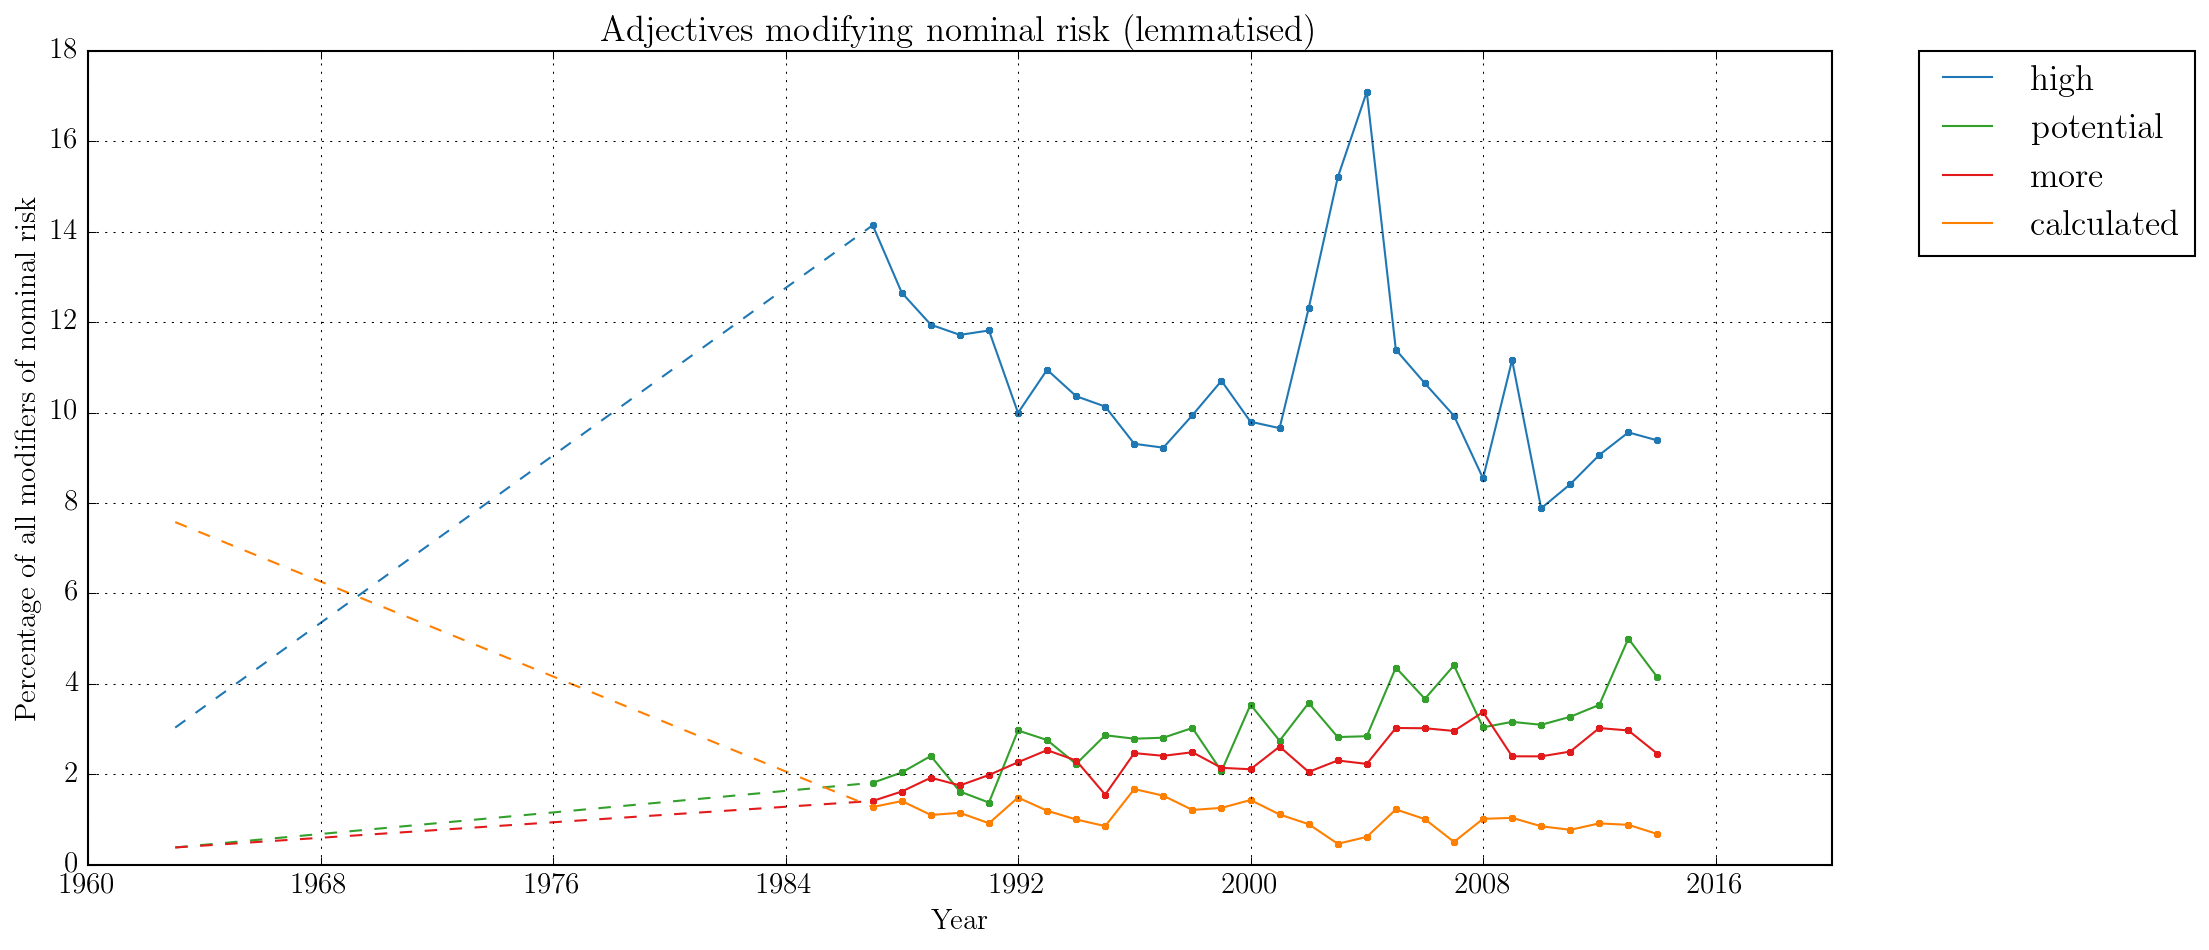
\includegraphics[width=0.75\textwidth]{../images/adjectives_modifying_nominal_risk_(lemmatised).png}
    \caption{Selected modifiers of participant risk as percentage of all risk modifiers}
    \label{fig:reladjrisk}
    \end{figure}

    %~\ \todo[inline,color=yellow!40]{\noindent Significance of this?}

    \vspace{5mm}\noindent\begin{tcolorbox}[colback=yellow!5,colframe=yellow!40!black,title=Summary: modifiers of risk as participant]
    \parbox{1\textwidth}{%
    \emph{Calculated risk} has been overtaken by \emph{potential risk} in overall frequency. \emph{High-risk} spikes in frequency in references to H5N1.}
    \end{tcolorbox}
    \vspace{5mm}


\section{What kinds of risk processes are there, and what are their relative frequencies?} \FloatBarrier

    Our second area of interest within the transitivity system is risk as a process. Within the corpus, we located five distinct risk processes. First, risk alone may be a process (\emph{I won't risk it}). Second and third are \emph{running risk} and \emph{taking risk}---\emph{process--range} configurations, where the verbal component is largely shorn of meaning, and with meaning conveyed primarily in the nominal in object position \cite{halliday_introduction_2004}. Fourth is \emph{putting somebody/something at risk}, which involves an obligatory nominal object argument and a prepositional-phrase complement. Finally, we have

    Other phrases sit on the cusp as recognisable risk processes: \emph{to carry risk}, for example, is frequent in the data, but we have not included it because we feel that the semantic burden of this process still lies in \emph{carry} (unlike \emph{pose} in \emph{to pose risk}).

    \begin{figure}[htb!]
    \centering
    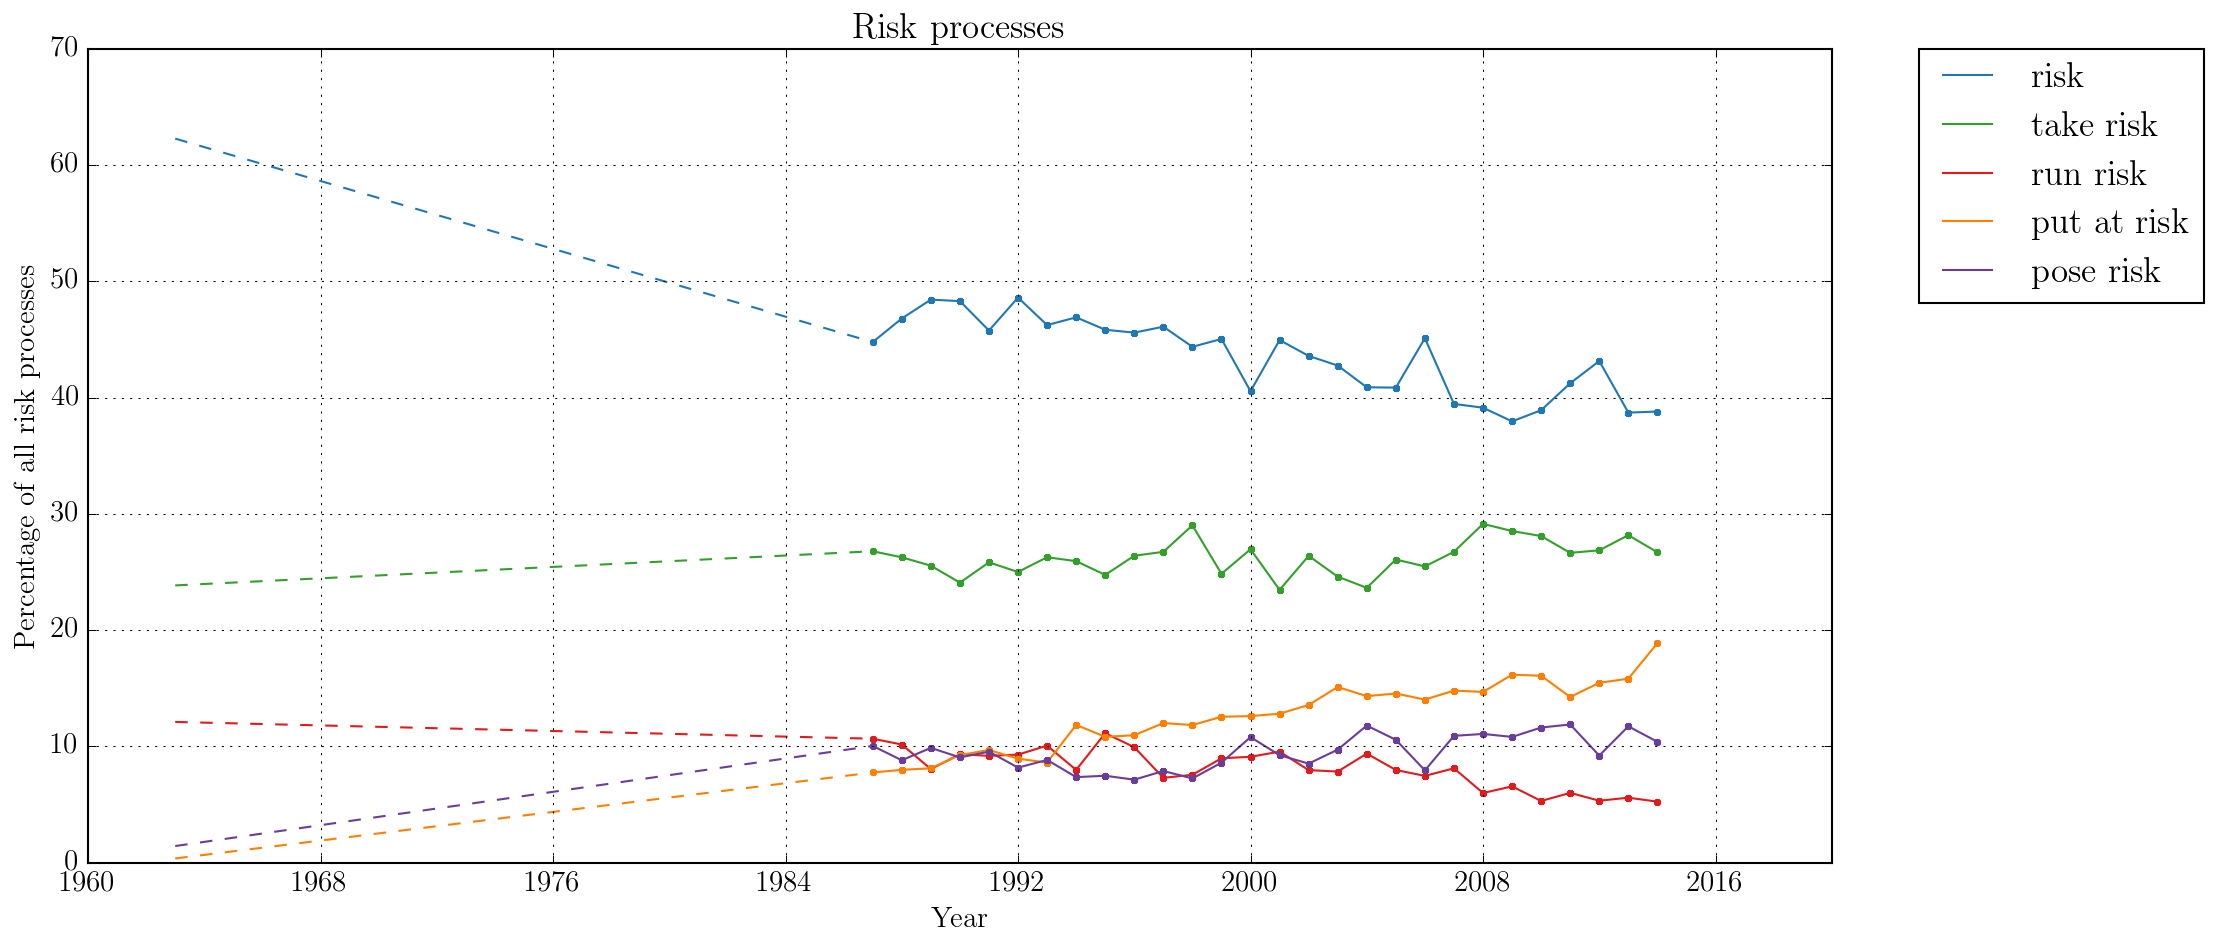
\includegraphics[width=0.75\textwidth]{../images/risk_processes.png}
    \caption{Risk processes as percentage of all parsed processes}
    \label{fig:riskprocesses}
    \end{figure}
    %
    Our first interest is the overall frequency of these five risk processes. 
    %From Figure \ref{fig:riskprocesses}, we concluded that risk processes generally are on an static\slash slightly outbound trajectory, with a notable decrease in frequency between the 1963--1987 samples.
    Figure \ref{fig:riskprocesses} charts the trajectory of the five identified risk processes. Most interesting here are that the `standard' (predicatorial) risk process is steadily decreasing, in favour of the other processes, each of which seems to provide additional connodations of the agency of the risker as well as his\slash her\slash its understanding of the level of risk. 

    The second notable finding here is that \emph{putting at risk} has overtaken \emph{running risk} in frequency.

    Concordancing revealed that in 2014, \emph{putting at risk} is used in cases where the potential harm is either implicit or explicit:

    \begin{enumerate}  [before=\itshape,font=\normalfont] \setlength\itemsep{0em} \small
    \item Ultimately, there is a price to pay: If you attack our soldiers, you're putting yourself at risk.
    \item But addicted health care workers need not be physicians to put patients at risk.
    \item While obviously no airline or company deliberately puts people at risk, `sometimes new risks are identified and steps have to be taken,' Mr. Koch said.
    \end{enumerate}

    \begin{enumerate}  [before=\itshape,font=\normalfont] \setlength\itemsep{0em} \small
    \item The auction houses deny that they are trimming profits with givebacks or putting themselves at financial risk.
    \item Rather, such tax status is generally put at risk when groups stray from their mission.
    \item They had handled her body, putting them at serious risk of infection.
    \end{enumerate}

    That said, we also noted that there seems to be some evidence for lessening agency in recent \emph{risk running} processes. Compare 1963 and 2014 results:

    \begin{enumerate} [before=\itshape,font=\normalfont]  \setlength\itemsep{0em} \small
    \item However, if adults decide to run a risk, this is up to them, and anyway, Switzerland adequately handles American affairs in Havana.
    \item In Washington at the weekend it was pretty welt agreed that the MIG incident was not deliberate provocation; the feeling was that, even with the Russian presence, Castro would not wilfully run the risk of American retaliation.
    \item  If he sticks to the more-or-less official Republican position against off-track betting, he runs the risk of losing thousands of New York City votes, which he needs.
    \end{enumerate}

    \begin{enumerate} [before=\itshape,font=\normalfont]   \setlength\itemsep{0em} \small
    \item Fans see this revolving door of injuries with so much regularity that they run the risk of becoming desensitized 
    \item `One runs the risk of falling for a voice.'
    \item `I would run the risk of having two boys,' she said.
    \item On the other hand, if Argentina does default, it runs the risk of more lawsuits, said Siobhan Morden, head of Latin America strategy at Jefferies.
    \item And, like an overdressed beachgoer, a classic cocktail served straight up runs a high risk of wilting in the sunshine.
    \end{enumerate}
    %
    Overall, the shift in both the semantics of risk running and the increasing preference for \emph{putting at risk} can be seen as evidence for decreasing agency in risk, as well as an increasing implicitness of the potential harm. This finding is especially significant, given that the existing descriptions of risk \cite{fillmore_toward_1992}, as well as the current FrameNet database, include accounts of \emph{running risk} as a frame, but not \emph{putting at risk}.

    \vspace{5mm}\noindent\begin{tcolorbox}[colback=yellow!5,colframe=yellow!40!black,title=Summary: types of risk processes]
    \parbox{1\textwidth}{%
    Both \emph{pose risk} and \emph{put at risk} have overtaken \emph{run risk} in frequency. Use of the prototypical risk process, \emph{to risk} is declining. Finally, there is some evidence for reduced agency the \emph{run risk} process.}
    \end{tcolorbox}
    \vspace{5mm}
    
\section{When risk is a process, what participants are involved?} \FloatBarrier
    
    Clauses containing risk processes are a rich site for analysis, as the semantic roles of participants are determined by their placement with respect to the process. Experiential subjects of risk processes can be mapped to \emph{riskers}. Experiential objects are either \emph{risked things} or \emph{potential harm} (\emph{they risked their lives/death}). Table \ref{tab:riskersx} lists the most common subject and object participants of risk processes. Also of interest are clauses embedded within risk processes (e.g. \emph{she risks hurting herself/losing her life}). Table \ref{alienating} lists the (lemmatised) top twenty subordinated processes in the corpus.

    \begin{table}[htb!]
    \centering
    \addvbuffer[12pt 8pt]{\begin{minipage}{.35\textwidth}
    \centering
    \small
    \begin{tabularx}{1.0\textwidth}{|>{\raggedright}l|X|}
    \hline
    \textbf{Risker}           & \textbf{Risked thing\slash potential harm} \\ \hline
    person & life \\ \hline
    company & injury \\ \hline
    state & loss \\ \hline
    woman & everything \\ \hline
    man & death \\ \hline
    investor & money \\ \hline
    bush & wound \\ \hline
    player & war \\ \hline
    government & career \\ \hline
    worker & arrest \\ \hline
    republican & health \\ \hline
    clinton & damage \\ \hline
    bank & reputation \\ \hline
    democrat & fine \\ \hline
    anyone & capital \\ \hline
    obama & future \\ \hline
    child & confrontation \\ \hline
    move & job \\ \hline
    firm & backlash \\ \hline
    administration & failure \\ \hline
    \end{tabularx}
    \caption{Riskers and risked things and\slash or potential harms}
    \label{tab:riskersx}

    \end{minipage}} \hspace{1cm} % This must go next to `\end{minipage}`
    \addvbuffer[12pt 8pt]{\begin{minipage}{.35\textwidth}

    \centering
    \small
    \begin{tabularx}{0.9\textwidth}{|l|X|}
    \hline
    \textbf{Embedded process}      & \textbf{Total ~~~~~~~~~~~~~~~~~~~~~~~~~~~~~~~~~~~~~~~~~~} \\ \hline
    lose      & 1260  \\ \hline
    be        & 1095  \\ \hline
    alienate  & 379   \\ \hline
    have      & 347   \\ \hline
    become    & 285   \\ \hline
    get       & 184   \\ \hline
    make      & 166   \\ \hline
    turn      & 119   \\ \hline
    go        & 113   \\ \hline
    offend    & 110   \\ \hline
    take      & 86    \\ \hline
    look      & 85    \\ \hline
    undermine & 82    \\ \hline
    anger     & 79    \\ \hline
    fall      & 78    \\ \hline
    create    & 76    \\ \hline
    put       & 74    \\ \hline
    miss      & 73    \\ \hline
    give      & 73    \\ \hline
    damage    & 62    \\ \hline
    \end{tabularx}
    \caption{Most common embedded processes in risk processes}
    \label{alienating}
    
    \end{minipage}}
    \end{table}

    Riskers are most typically powerful institutions or individuals. Risked things and potential harms are generally serious and grave. A mismatch occurs here: \emph{Bush} and \emph{Obama} do not likely risk \emph{wounds}, \emph{arrest} or \emph{death}. In terms of subordinated processes, notable is the appearance of processes that are fairly uncommon: \emph{alienating}, \emph{offending}, \emph{undermining} and \emph{angering} and are three key examples, ranking amongst expected processes like \emph{being}, \emph{having}, \emph{getting}, \emph{making} and \emph{going}. Without considering longitudinal change, we can see from this that the embedded processes are often related to more powerful social actors: states, political parties and politicians risk alienating electorates; diplomats risk offending one another. Even embedded processes lacking explicit connotations of power are typically deployed in the contexts of government, industry or society. Below are concordance results for \emph{risk alienating} in 2013, which appears 14 times.


    \begin{figure}
    \footnotesize
    \begin{tabular}{rcl}
    stoked further concerns that unemployment risked &  becoming &  endemic and could eventually cause social upheaval  \\ 
    franchise, the stage scene could have risked &  becoming &  an embarrassment for the brand, but Mr. Timbers'   \\ 
    with locally, or else the Vatican offices risk &  becoming &  institutions of censorship   \\ 
    on which the experience depends -- or risk &  becoming &  irrelevant to future generations, Mr. Staggs said   \\ 
    restart growth, warning that the euro area risked &  becoming &  mired in the same kind of economic stagnation that   \\ 
    If left unaddressed, such practices risk &  becoming &  more and more entrenched, Ann Harrison of   \\ 
    without serious savings in this area, we risk &  becoming &  an unbalanced force, one that is well compensated   \\ 
    Switzerland risks &  becoming &  one of the most restrictive places for management   \\ 
    What was the exception before now risks &  becoming &  the standard practice   \\ 
    the pope's new remarks that the church risked &  becoming &  a `small chapel' overly fixated on sexual   \\ 
    hailed the step as significant, it risks &  becoming &  the latest of many tentative moves toward talks   \\ 
    Rather than race the clock to Bed-Stuy and risk &  becoming &  an early bike-share casualty, I stopped at a   \\ 
    increasingly turning to what, strangely, risked &  becoming &  the most marginalized group of all: the bosses   \\ 
    and currency crisis in the European Union risks &  becoming &  a crisis of liberal democracy itself \\ 
    \end{tabular}
    \caption{\emph{To risk becoming} in 2013 subcorpus}
    \end{figure}
    

    %DEPENDING ON HOW MUCH TIME THERE IS, I COULD SEARCH FOR ALL OF THE RISKERS INDIVIDUALLY...

    %Though these objects may be grammatically ambiguous, the function of the object can be disambiguated by inserting \emph{losing}.

    %\begin{enumerate}	\setlength\itemsep{0em}
    %\item He risked his life
    %\item He risked losing his life
    %\item He risked death
    %\item * He risked losing death
    %\end{enumerate}

    %Note here an emerging methodological issue: the various  \emph{potential harms} can also be located by querying nominal risks (e.g. \emph{the risk of death}). Some methodological adaptability is thus required.

    \vspace{5mm}\noindent\begin{tcolorbox}[colback=yellow!5,colframe=yellow!40!black,title=Summary: participants in risk processes]
    \parbox{1\textwidth}{%
    When risk is a process, risked things\slash potential harms often pertain to individual health (\emph{to risk life, death, health, etc.}). This contrasts with processes as potential harm, which generally relate to people in positions of power (\emph{to risk alienating voters}, for example).}
    \end{tcolorbox}
    \vspace{5mm}

\section{When risk is a modifier, what are the most common forms?} \label{sect:riskmod} \FloatBarrier

    \begin{table}
    \small
    \centering
    \begin{tabular}{|l|l|}
    \hline
    \textbf{Modifier type}       & \textbf{Example}          \\ \hline
    Adjectival pre-head & \emph{a risky move}     \\ \hline
    Post-head           & \emph{A person at risk} \\ \hline
    pre-head nominal    & \emph{risk management}  \\ \hline
    Adverbial           & \emph{to riskily act}   \\ \hline
    Circumstance head   & \emph{to be at risk }   \\ \hline
    \end{tabular}
    \caption{Types of risk-as-modifier}
    \label{tab:modriskwords}
    \end{table}

    There are many different kinds of risk as modifier (see Table \ref{tab:modriskwords} for a non-exhaustive list of examples). Our first interest was in gauging the prevalence of the different forms. From this query, we noted that pre-head nominal modifiers are increasing in frequency. A good example is \emph{risk factor} (see Figure \ref{fig:riskfactor}).


    \noindent
    \begin{figure}[htb!]
    \centering
    \begin{minipage}{.567\textwidth}
    \centering
    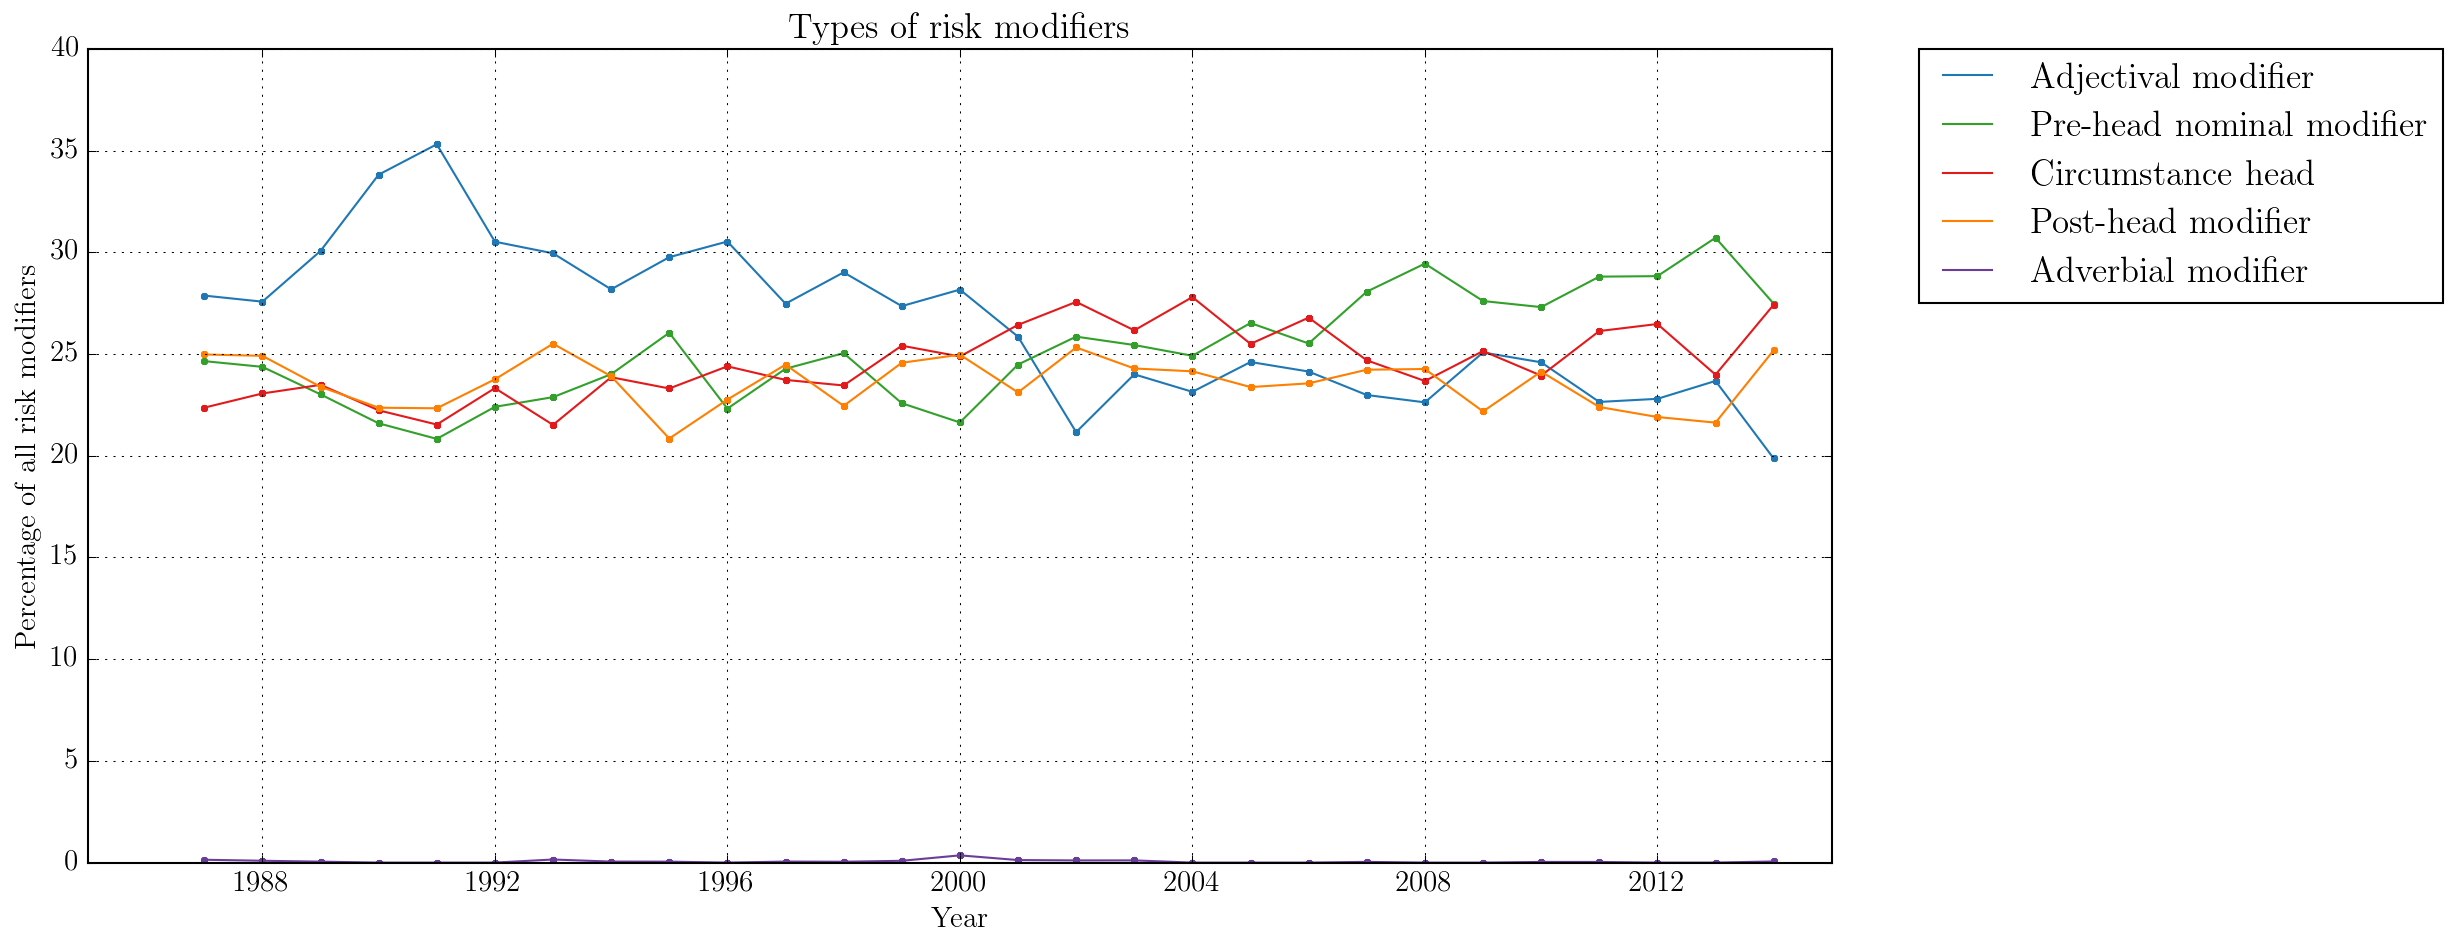
\includegraphics[width=0.98\textwidth]{../images/types-of-risk-modifiers.png}
    \captionof{figure}{Types of risk modifier}
    \label{fig:riskmod_types}
    \end{minipage}%
    \begin{minipage}{.433\textwidth}
    \centering
    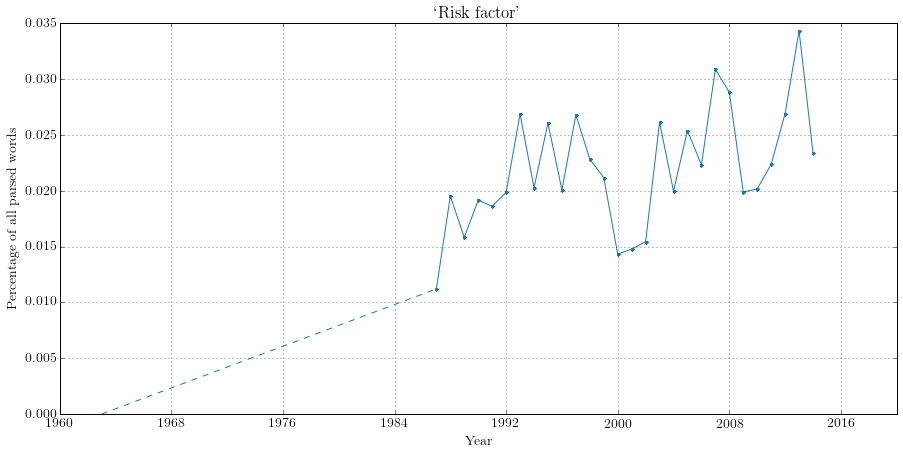
\includegraphics[width=0.98\textwidth]{../images/risk-factor.png}
    \captionof{figure}{Relative frequency of \emph{risk factor}}
    \label{fig:riskfactor}
    \end{minipage}
    \end{figure}


    Modifier risks are unique for their variety and diversity: through compounding, comprehensible new risk words and phrases can easily be created. The entire corpus contained 327 unique adjectival risk words, including \emph{non-risk}, \emph{de-risk}, \emph{once-risky}, \emph{take-no-risks}, \emph{risk-swapping}, \emph{risk-abhorrent}, \emph{price-for-risk}, \emph{post-risky}, \emph{pooled-risk}, \emph{personal-risk}, \emph{optimum-risk}, \emph{one-risk-factor}, \emph{one-pitch-can-end-his-career-risk} and \emph{low-risk-to-society}. That said, most of these occur no more than a handful of times. By far the most common were \emph{risky\slash riskier\slash riskiest} (15588 occurrences), \emph{high-risk} (5533), \emph{low-risk} (1086), \emph{at-risk} (902), \emph{risk-free} (883) and \emph{risk-taking} (789). Of these, four exhibited trajectory shifts (see Figure \ref{fig:adjtraj}). The basic adjectival forms (\emph{risky}, \emph{riskier}, \emph{riskiest}) are dominant in the 1963 sample, then decrease, and re-emerge in 2000. \emph{High-risk} though very rare (two instances) in 1963, has become more common, and stabilised in trajectory. \emph{Low-risk} and \emph{at-risk} are on a consistent inbound trajectory.

    \noindent
    \begin{figure}[htb!]
    \centering
    \begin{minipage}{.48\textwidth}
    \centering
    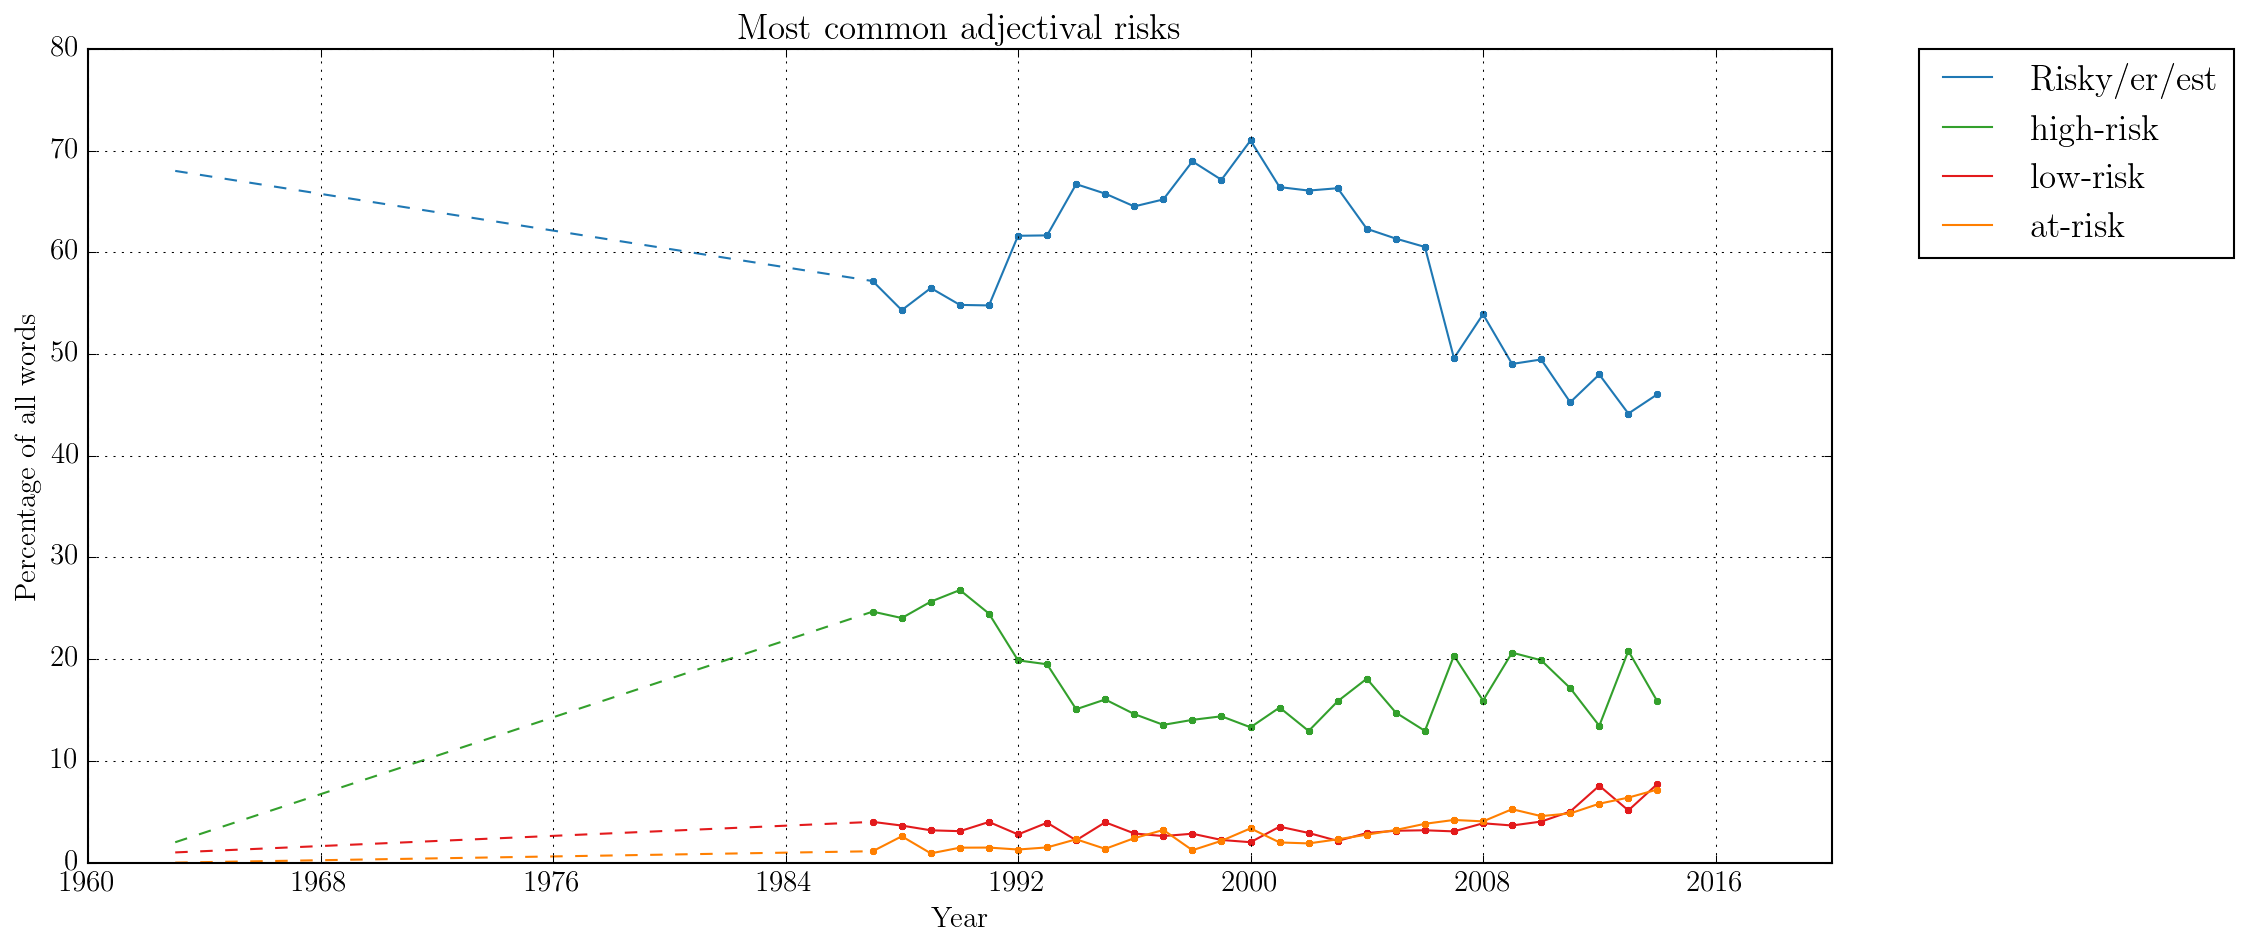
\includegraphics[width=0.98\textwidth]{../images/most_common_adjectival_risks.png}
    \end{minipage}%
    \begin{minipage}{.48\textwidth}
    \centering
    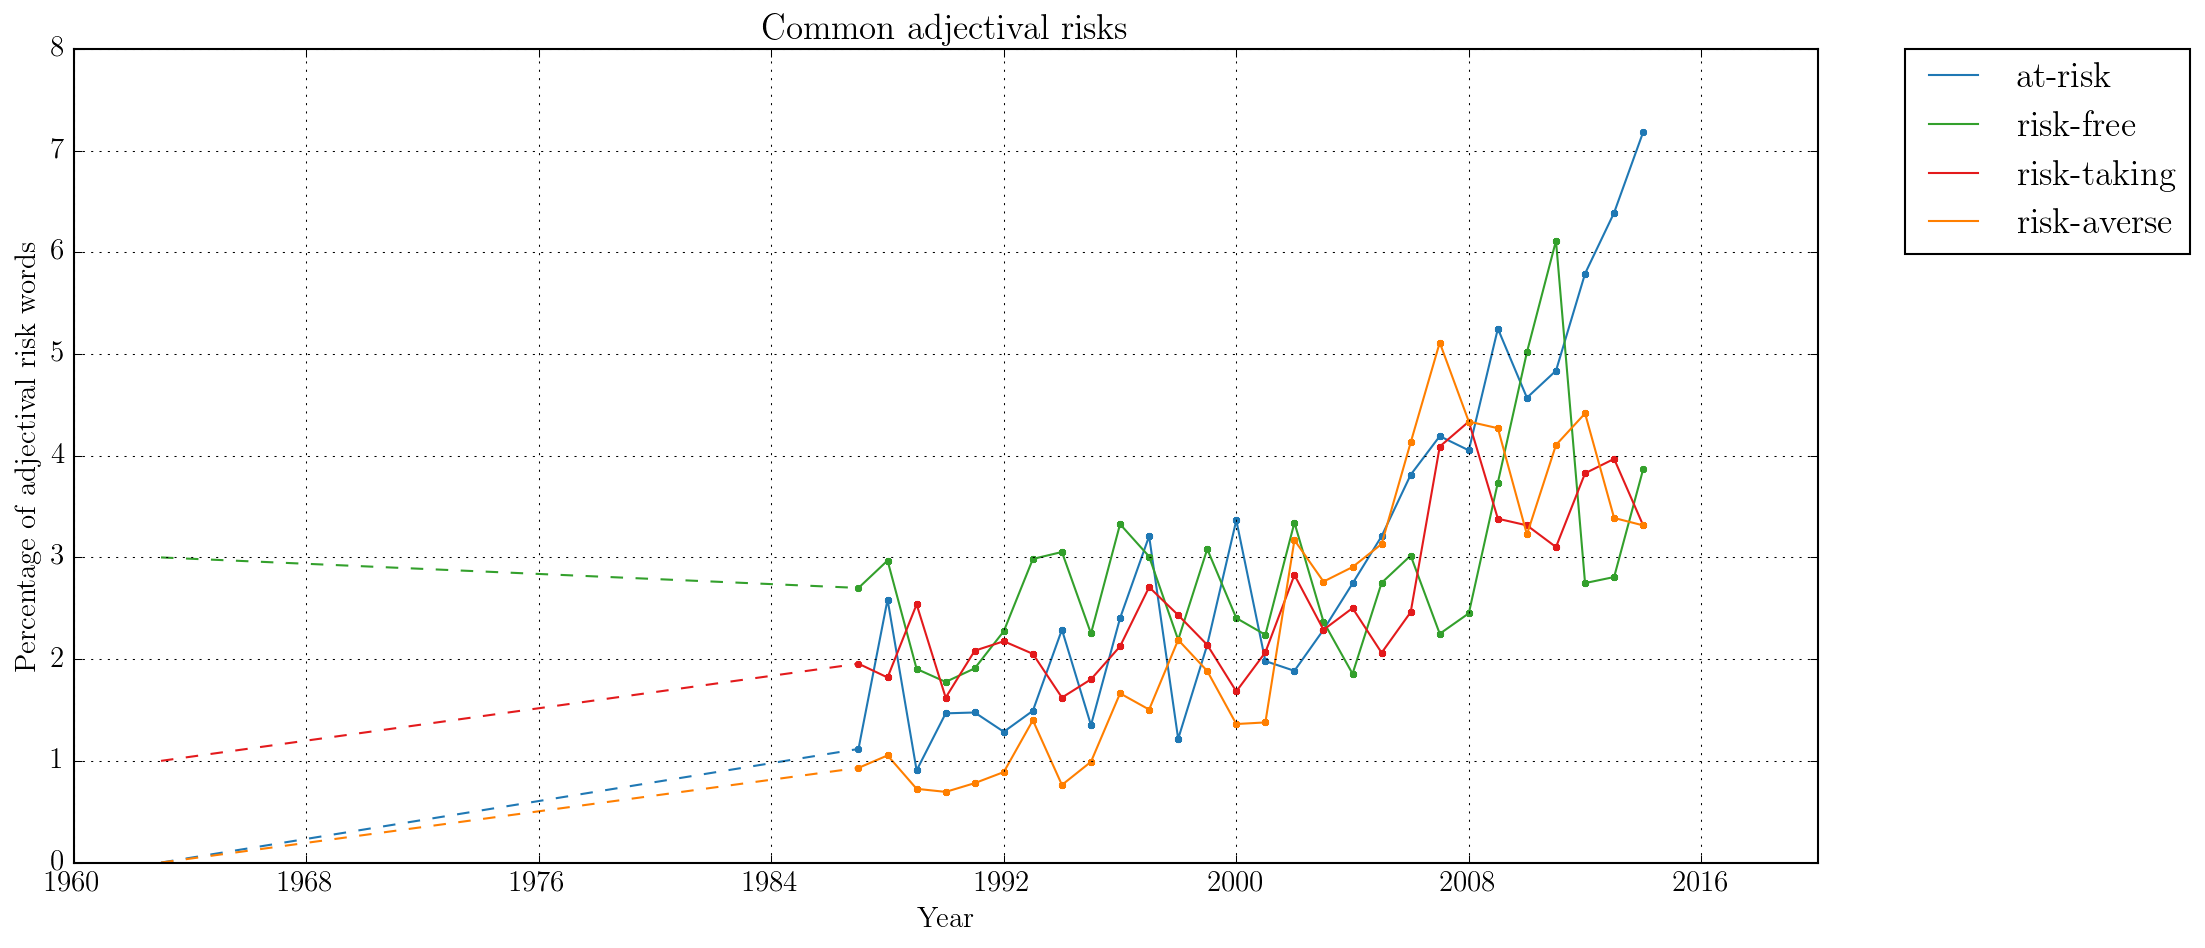
\includegraphics[width=0.98\textwidth]{../images/common_adjectival_risks.png}
    \end{minipage}
    \caption{Common adjectival risk words as percentage of all adjectival risks}
    \label{fig:adjtraj}
    \end{figure}

    The prevalence of high-risk in the 1980s is largely due to the AIDS epidemic: concordancing reveals that certain populations (gays, African Americans, Haitians) are at high-risk of being inflected by HIV. \emph{At-risk} is rare in earlier editions, but increases in prevalence steadily.

    This shift in risk is modifier is an important one. Low, moderate and high risk comprises a gradient, or scale, while at-risk is a binary. As with the shift toward \emph{potential risk}, this indicates both an increasing pervasiveness and a decreasing calcuability of risk. %remember that low-risk is actually increasing.
    
    %Of the graduated risks, low-risk is the only one on an inbound trajectory. What's the significance of this?



    %For people at moderate risk who also have two of the other risk factors , the treatment should be the same as for those in the high-risk group .
    %But ecologists , doctors and other specialists here warn that the entire population , not just high-risk groups , is vulnerable .
    %In the weeks since the law took effect , couples seeking marriage licenses have besieged hospitals , clinics and other doctors , anxious to get the test and the required counseling in time for wedding dates and quickly outnumbering those in high-risk groups most in need of attention .
    %Health experts say scarce funds for AIDS prevention would be better spent on high-risk groups .
    %Very few Americans know that Haitians have long since been removed from the list of high-risk groups because it was discovered that the H

    \vspace{5mm}\noindent\begin{tcolorbox}[colback=yellow!5,colframe=yellow!40!black,title=Summary: frequencies of modifier risk]
    \parbox{1\textwidth}{%
    Common risk modifiers (\emph{risky}, \emph{riskier}, \emph{riskiest}) are gradually being displaced by a number of less common constructions (e.g. \emph{low-risk}, \emph{at-risk}, \emph{risk-averse}, \emph{risk-free}).}
    \end{tcolorbox}
    \vspace{5mm}

\section{When risk is a modifier, what is being modified?} \FloatBarrier

    Risk as a modifier can be placed either before or after the noun it modifies (\emph{an at-risk person\slash a person at risk}). These two constructions are collapsed in Tables \ref{tab:riskmodified} and \ref{tab:atrisk}, which respectively list the participants most frequently modified by any risk modifier, and the participants most frequently modified by \emph{at-risk\slash at risk}. Note that while risk-modified participants generally are financial and economic in nature (\emph{investment, business, loan, asset}), the at-risk subset is mainly comprised of vulnerable populations of people (\emph{women}, \emph{children}, \emph{students}).

    \begin{table}[htb!]
    \centering
    \addvbuffer[12pt 8pt]{\begin{minipage}{.37\textwidth}
    \centering
    \small
    \begin{tabularx}{1.0\textwidth}{|X|l|}
    \hline
    \textbf{Risk-modified \mbox{participant}}        & \textbf{Total} \\ \hline
    investment  & 696   \\ \hline
    business    & 515   \\ \hline
    behavior    & 508   \\ \hline
    group       & 466   \\ \hline
    loan        & 421   \\ \hline
    asset       & 388   \\ \hline
    strategy    & 377   \\ \hline
    bond        & 346   \\ \hline
    area        & 307   \\ \hline
    venture     & 301   \\ \hline
    security    & 287   \\ \hline
    patient     & 265   \\ \hline
    pool        & 239   \\ \hline
    bet         & 214   \\ \hline
    move        & 204   \\ \hline
    activity    & 201   \\ \hline
    proposition & 199   \\ \hline
    child       & 170   \\ \hline
    woman       & 161   \\ \hline
    student     & 158   \\ \hline
    \end{tabularx}
    \caption{Most common risk-modified participants in the corpus}
    \label{tab:riskmodified}
    \end{minipage}} \hspace{1cm}
    \addvbuffer[12pt 8pt]{\begin{minipage}{.37\textwidth}
    \small
    \begin{tabularx}{1.0\textwidth}{|X|l|}
    \hline
    \textbf{At-risk \mbox{participant}}       & \textbf{Total} \\ \hline
    person     & 439   \\ \hline
    child      & 368   \\ \hline
    woman      & 209   \\ \hline
    student    & 179   \\ \hline
    nation     & 135   \\ \hline
    patient    & 110   \\ \hline
    youngster  & 93    \\ \hline
    group      & 91    \\ \hline
    population & 64    \\ \hline
    family     & 58    \\ \hline
    kid        & 50    \\ \hline
    youth      & 48    \\ \hline
    money      & 48    \\ \hline
    worker     & 45    \\ \hline
    life       & 41    \\ \hline
    job        & 41    \\ \hline
    man        & 40    \\ \hline
    area       & 35    \\ \hline
    teenager   & 32    \\ \hline
    other & 32 \\ \hline
    \end{tabularx}
    \caption{Most common at-risk participants in the corpus}
    \label{tab:atrisk}
    \end{minipage}}% This must go next to `\end{minipage}`
    \end{table}

    In need of further research is whether or not the list of entities that can sensibly be modified by \emph{at-risk} is beginning to grow: since the U.S. subprime mortgage crisis (beginning in 2007), references to \emph{at-risk homeowners} appear to be on the rise. Results from 2011, for example, show that \emph{nations} and even \emph{economic sectors} are being modified with \emph{at-risk}:

    \begin{enumerate}  [before=\itshape,font=\normalfont] \setlength\itemsep{0em} \small
    \item Mr. Obama asked for \$400 million for the World Bank's clean technology fund, \$95 million for the bank's program to prevent deforestation and \$90 million for its program to help at-risk nations cope with the effects of a warming planet by, for instance, developing drought-resistant crops.
    \item The most at-risk sectors included auto components and automobile companies, which generate nearly 30 percent of their sales in Europe, as well as food and tobacco firms.
    \end{enumerate}

    Note that it is difficult to reconcile the semantic meaning of \emph{at-risk} constructions with the semantic frame of risk provided by \citeA{fillmore_toward_1992}. Though elements of both the \textsc{victim} and \emph{valued object} appear to be at work, neither provides an adequate label for \emph{at-risk people, children, homeowners or nations}. Rather than being an oversight during the articulation of the risk frame (recall Figure~\ref{fig:fil_atk}), in light of the increased use of these kinds of constructions since the mid 1990s, we hypothesise that \emph{at-risk} constructions (as well as \emph{to put at risk}) are demonstrative of a broader shift in risk discourse toward general clusters of negative outcomes, rather than specific and measurable potential harms. Connection between this shift and sociological theory is made in the following chapter.

    \vspace{5mm}\noindent\begin{tcolorbox}[colback=yellow!5,colframe=yellow!40!black,title=Summary: participants modified by risk]
    \parbox{1\textwidth}{%
    While risk as a modifier is often used in the context of finance\slash commerce, \emph{at-risk} typically attaches to vulnerable human demographics.}
    \end{tcolorbox}
    \vspace{5mm}

\section{How arguable is risk?} \label{sect:arguability} \FloatBarrier

    As noted earlier, our central concern with the Mood system is the degree of arguability associated with the concept of risk. Risk in Subject, Finite and Predicator positions is the most arguable. Risk words within Complements and Adjuncts are less arguable.

    %A dependency grammar attempts to locate a lexical root for each clause, and attach dependents to it recursively until no lexical items are unattached. Each word is ordered by its dependency to the root of a clause. The nature of the dependency relationship can also be provided. Such grammars are particularly useful for free word order language, but have been applied to English successfully as well.

    Based on the kinds of parsing provided by Stanford CoreNLP, it was possible to measure arguability in two ways. First, we can map dependency relationships to the systemic-functional notion of arguability. A dependency grammar locates the predicator of a clause and assigns it a position of zero. A `1' is then assigned to its most immediate dependent (other components in the verbal group, if present, or the head of the Subject, if not). This process continues until no lexical items are unattached, or `ungoverned'. In effect, the higher the number attached to a word, the further it is semantically from being an important component in the meaning, and thus, in systemic functional terms, the less arguable the word.

    \begin{figure}[htb!]
    \centering
    \addvbuffer[12pt 8pt]{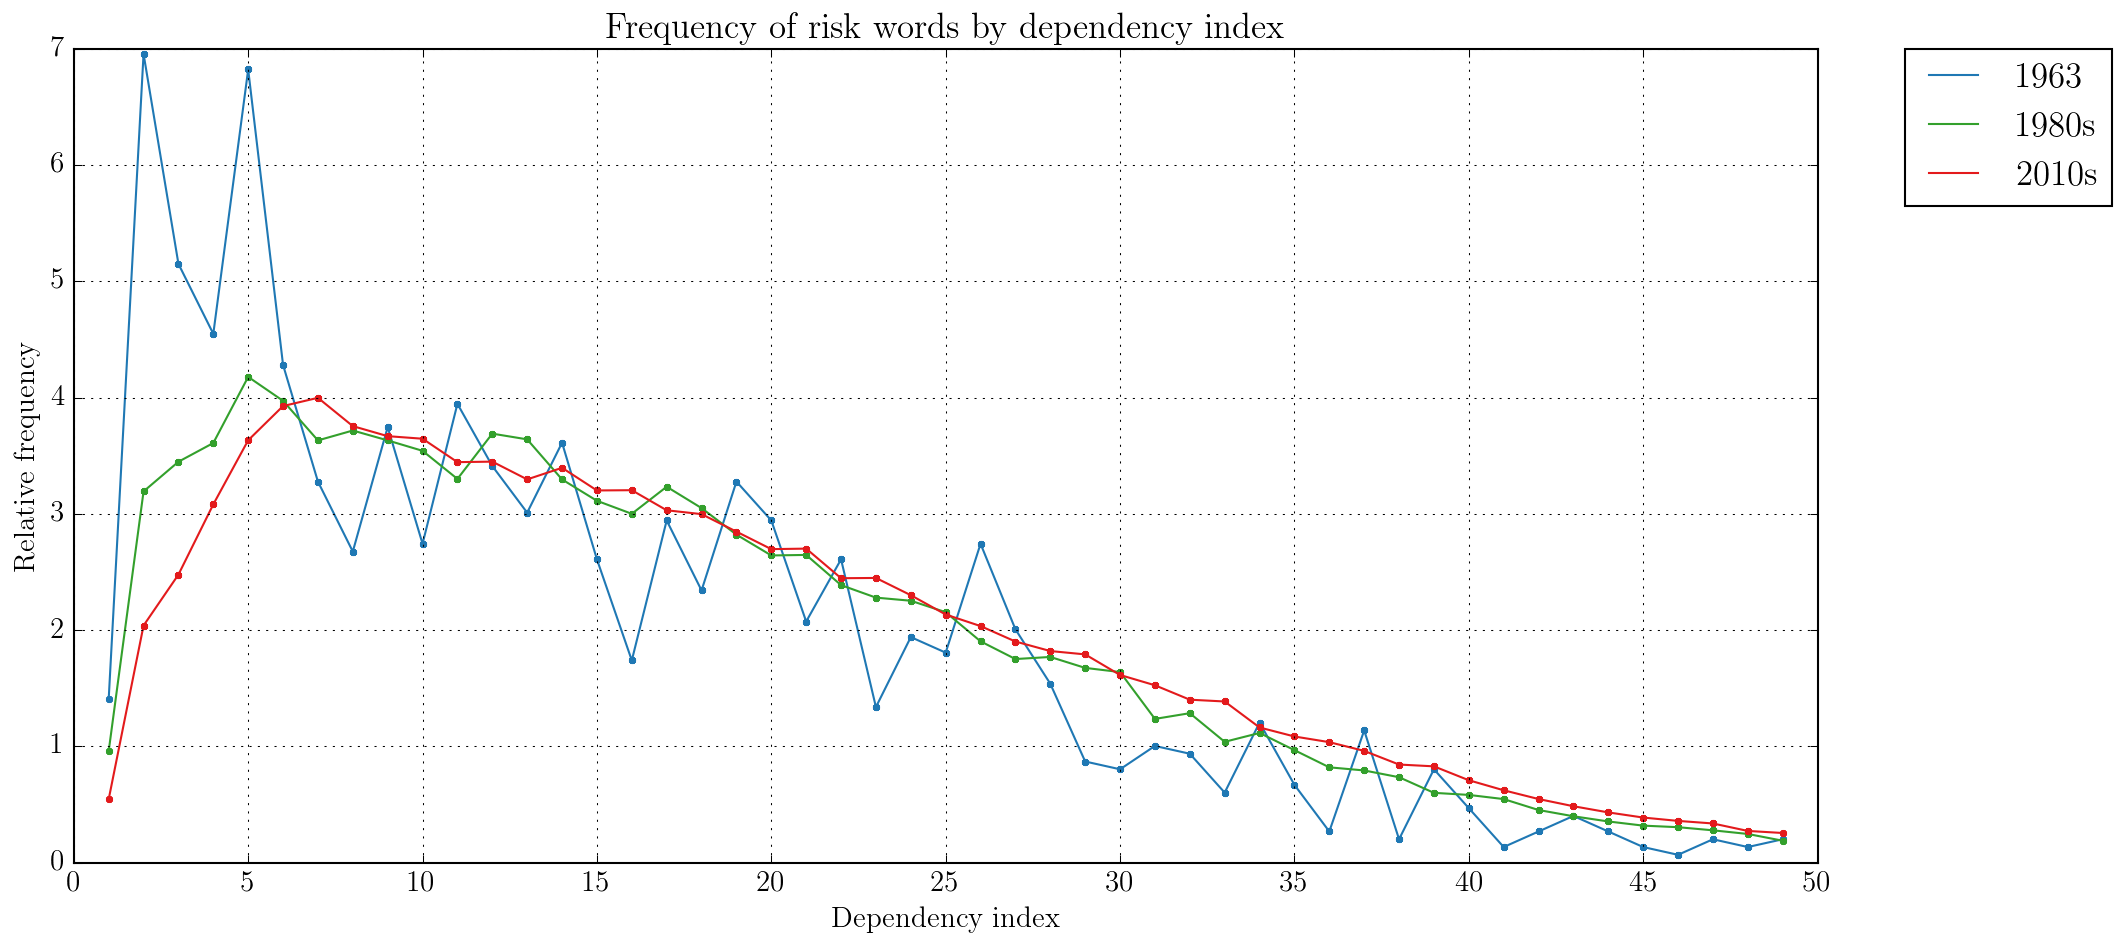
\includegraphics[width=0.75\textwidth]{../images/frequency-of-risk-words-by-dependency-index.png}}
    \caption{Risk words by dependency position in clause}
    \label{fig:depnum}
    \end{figure}
    %
    Highlighting three sampling periods as in Figure \ref{fig:depnum} shows that in early samples, risk occupies core roles within the dependency hierarchy, and thus sits closer to the core part of the meaning being exchanged within the clause. In later samples, risk more commonly occurs later in the dependency structure, in less focial positions. As explained earlier, though this experimental method is not a perfectly reliable indicators of arguability, it does indicate an increasing preference to position risk as non-core, ancillary information, rather than as the main thing which is under discussion.

    %\endnote{Dependency place 2 and 3 removed from visualisation, as these roles are typically for finites and modal auxiliaries---positions that a risk word cannot grammatically fill.}

    The second thing we can use dependency output for is identifying the functional roles of risk words. This is more accurate than using the dependency ranking, but creates a long list of functional roles. Of key interest, however, are risk words at the head of each major component of the Mood system---Subject, Finite\slash Predicator, Complement and Adjunct (CoreNLP parses unfortunately do not distinguish between Finite and Predicator in a reliable way, so the categories are collapsed here). From Figure \ref{fig:interpersonalarg}, we can see that risk is shifting from Subject and Finite\slash Predicator to Complement and Adjunct roles. This is an important result: risk words in more arguable roles are steadily decreasing, while risk in less arguable roles are becoming more common. Like earlier findings, this suggests an increasing implicitness of risk in NYT discourse, with less talk actually \emph{about} risk, but more talk where the relationship between risk and the subjects of the talk is assumed to be more or less common knowledge.

    \noindent
    \begin{figure}[htb!]
    \centering
    \begin{minipage}{.48\textwidth}
    \centering
    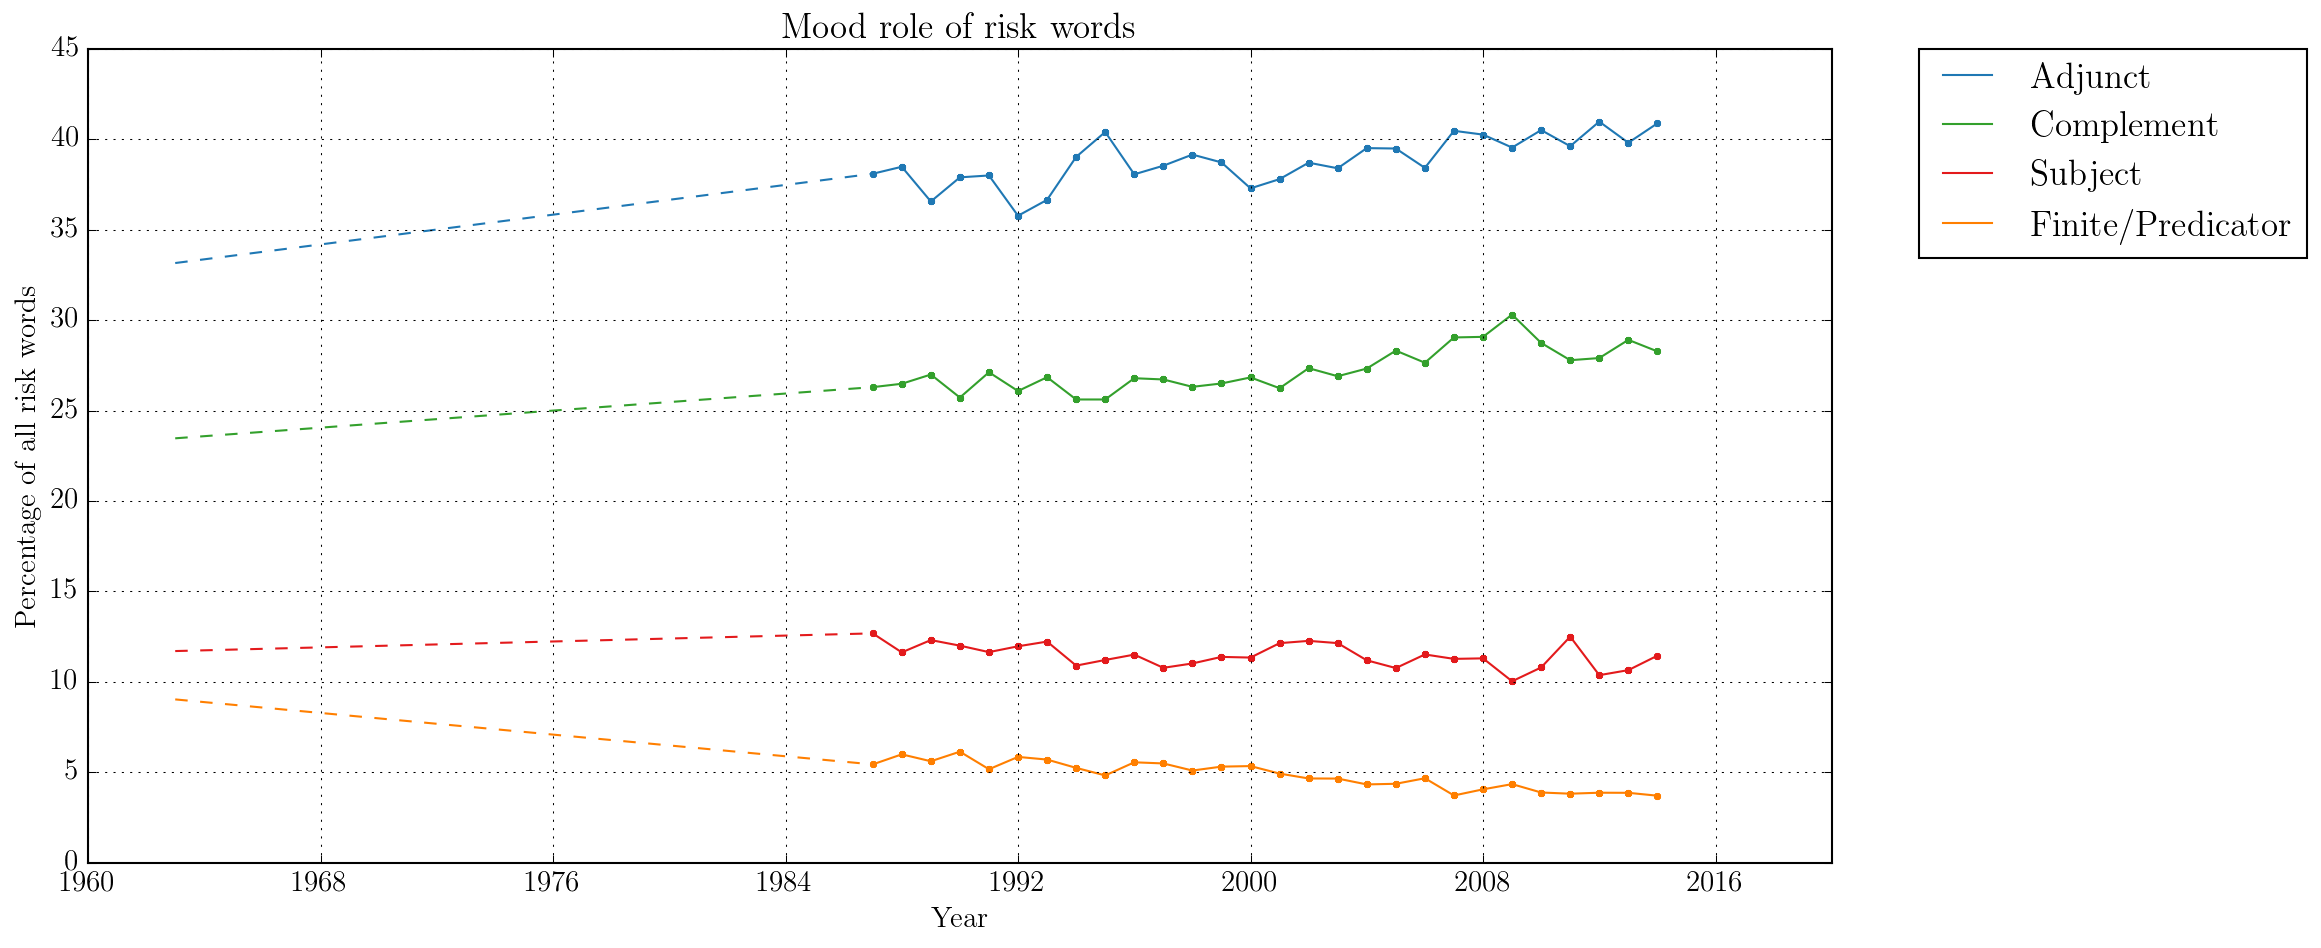
\includegraphics[width=0.98\textwidth]{../images/mood_role_of_risk_words.png}
    \end{minipage}%
    \begin{minipage}{.48\textwidth}
    \centering
    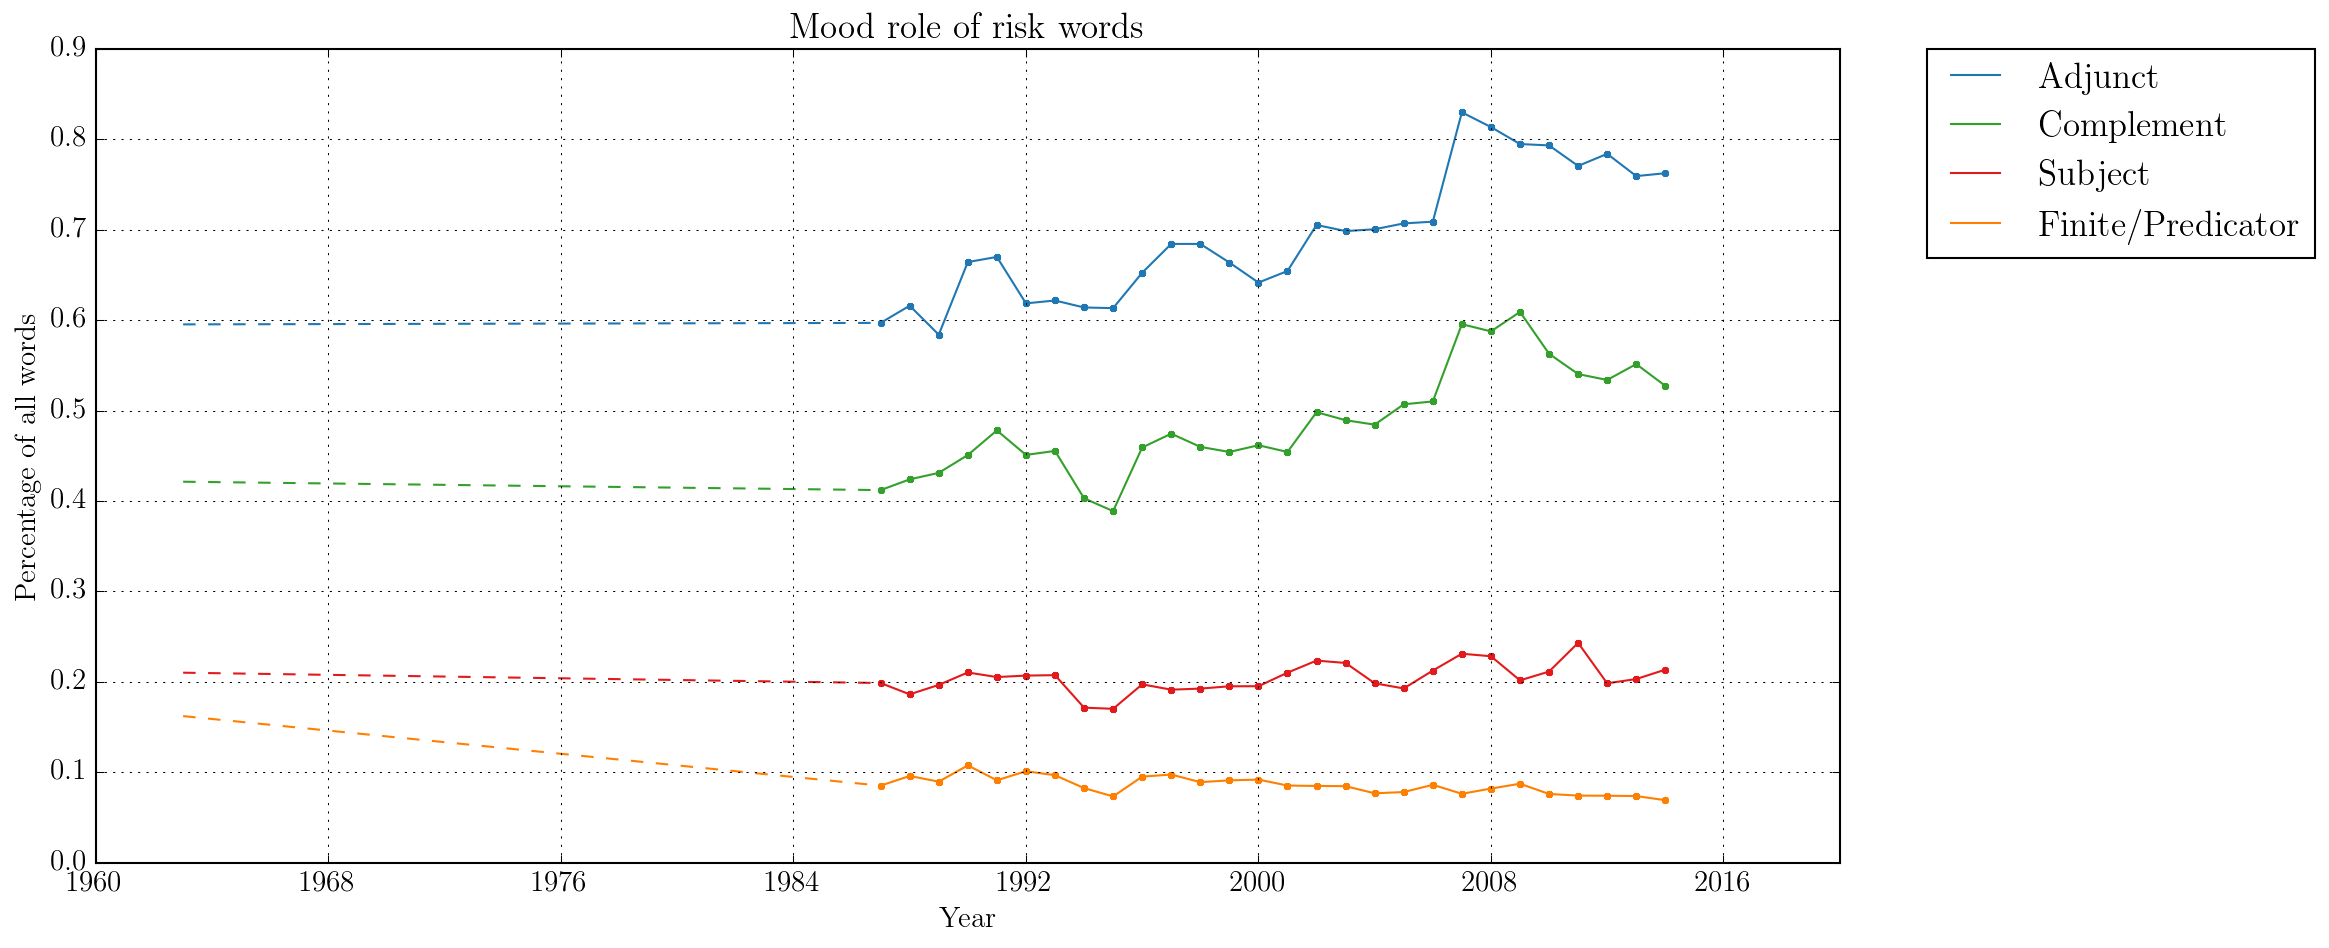
\includegraphics[width=0.98\textwidth]{../images/riskdep_allwords.png}
    \end{minipage}
    \caption{Frequency of risk words for each Mood component as percentage of all risk words\slash all parsed data}
    \label{fig:interpersonalarg}
    \end{figure}

    %By providing each role with a relative weight, we can plot arguability as a single decreasing trend line, showing the increased implicitness of risk within the language of the NYT.

    %Using the full list of risk dependencies, we can also locate more specific constructions undergoing trajectory shift. Figure \ref{fig:salienttrajectories} shows that risk is increasingly instantiated within prepositional phrases (which are by their nature dependent on Participants and Processes), and decreasingly as a predicator. From this view too, risk words are increasingly implicit within news language.

    \vspace{5mm}\noindent\begin{tcolorbox}[colback=yellow!5,colframe=yellow!40!black,title=Summary: risk and arguability]
    \parbox{1\textwidth}{%
    Longitudinally, risk words are shifting to less focal parts of clauses. We can approximate these changes using both indices or semantic function information within dependency parses.}
    \end{tcolorbox}
    \vspace{5mm}

\section{Risk words and proper nouns} \FloatBarrier

    We searched for proper noun groups in parse trees containing a risk word. This is a departure from many of our earlier queries, as here we are looking only at which entities co-occur with risk language, rather than determining how risk words and non-risk words relate to other another lexicogrammatically. The result of this query was 68891 different proper noun groups. We took the 200 most common results, and merged any that denoted the same entity: \emph{F.D.A.\slash Food and Drug Administration}, or \emph{Federal Reserve and Fed}. We then grouped results into thematic categories: \emph{People}, \emph{Nations}, \emph{Geopolitical entities}, \emph{Companies}, \emph{Organisations} and \emph{Medical themes}. The results were then plotted (See Figure \ref{fig:propernouns}). 

    \begin{landscape}
    \centering
    \begin{figure}
    \captionsetup[subfigure]{oneside,margin={-1.5cm,-.5cm}}
    \centering % [t!] % "[t!]" placement specifier just for this example
    \begin{subfigure}{.64\textwidth}
    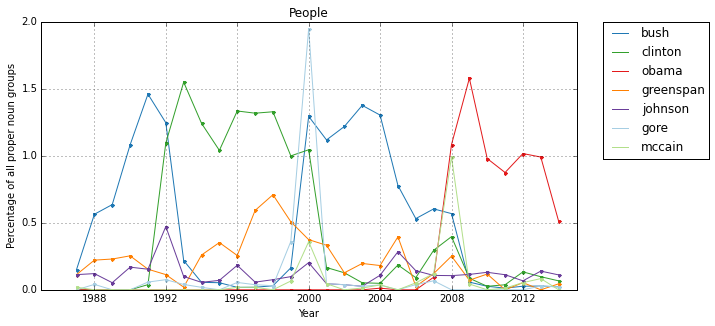
\includegraphics[width=\linewidth]{../images/people}
    \caption{People} \label{fig:a}
    \end{subfigure}
    \begin{subfigure}{.64\textwidth}
    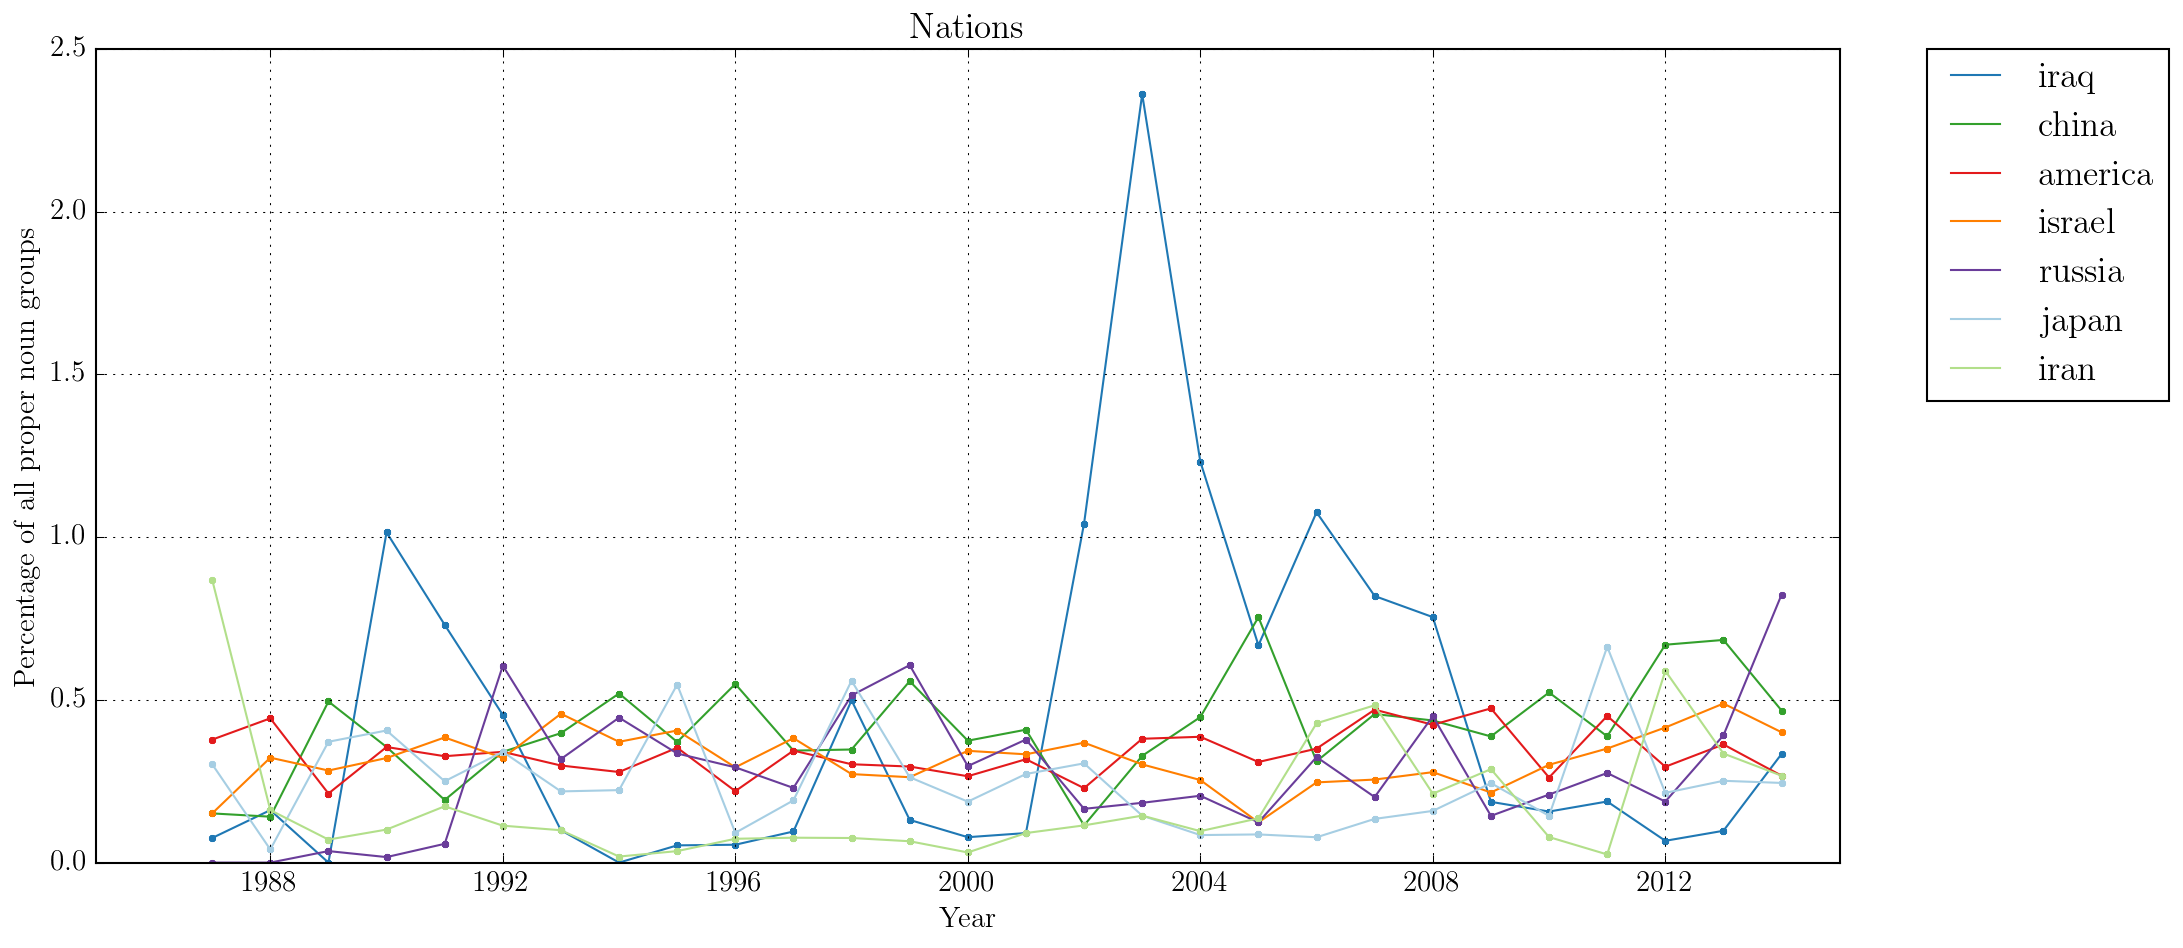
\includegraphics[width=\linewidth]{../images/nations}
    \caption{Nations} \label{fig:b}
    \end{subfigure}

    \medskip
    \begin{subfigure}{.64\textwidth}
    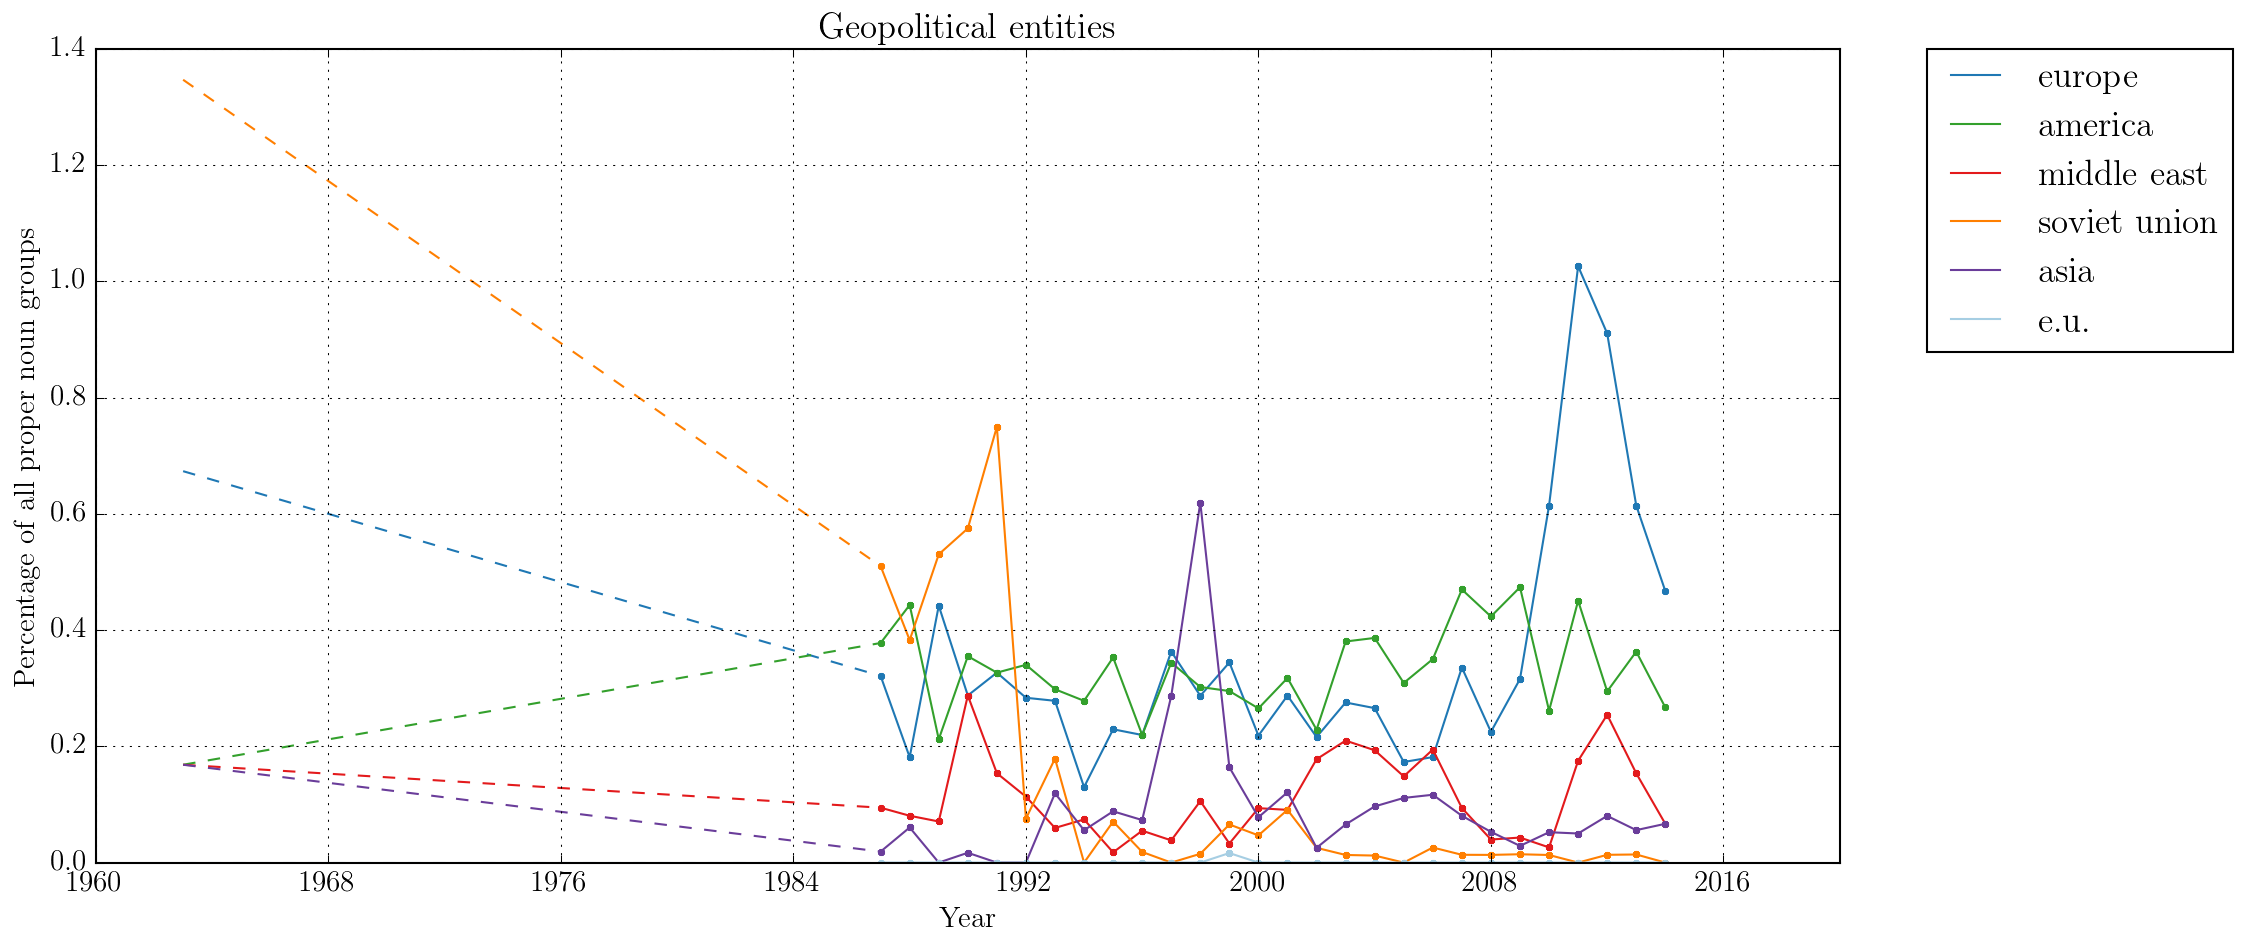
\includegraphics[width=\linewidth]{../images/geopolitical_entities}
    \caption{Geopolitical entities} \label{fig:c}
    \end{subfigure}
    \begin{subfigure}{.64\textwidth}
    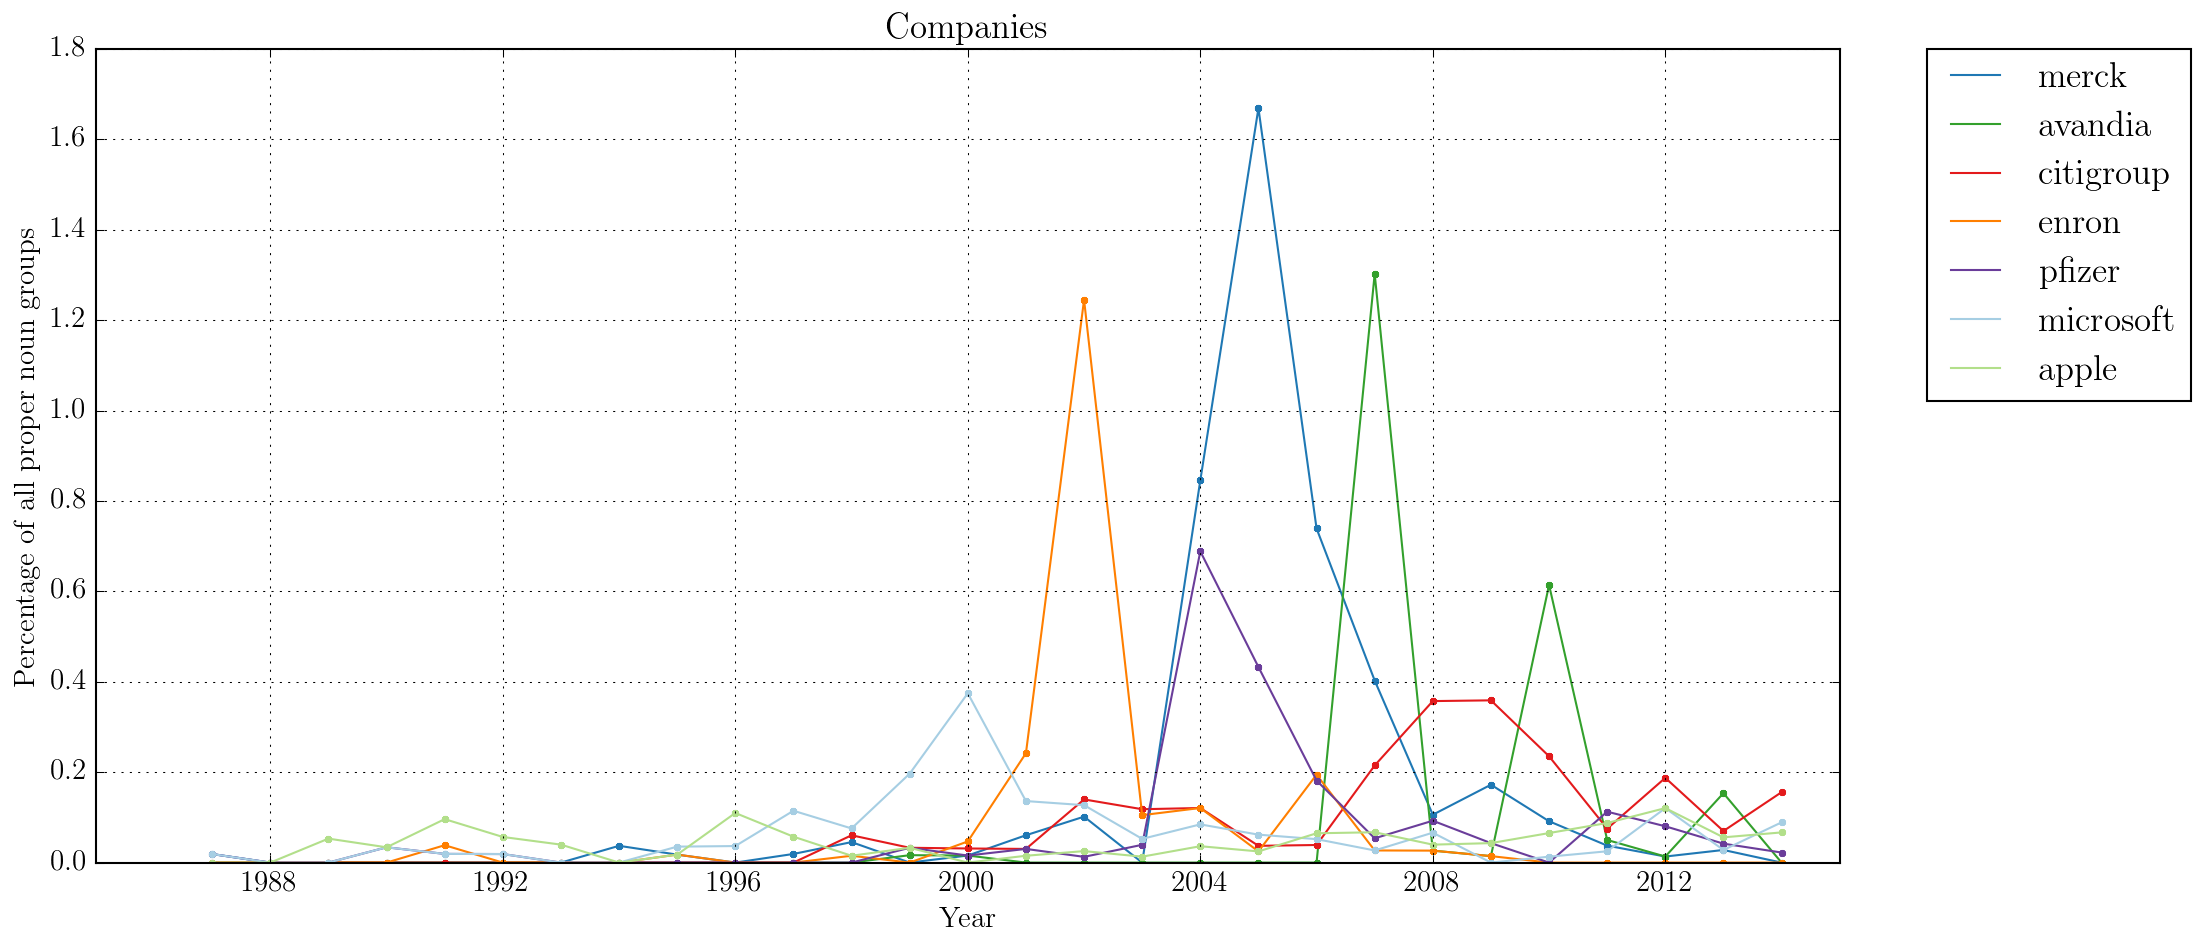
\includegraphics[width=\linewidth]{../images/companies}
    \caption{Companies} \label{fig:d}
    \end{subfigure}

    \medskip
    \begin{subfigure}{.64\textwidth}
    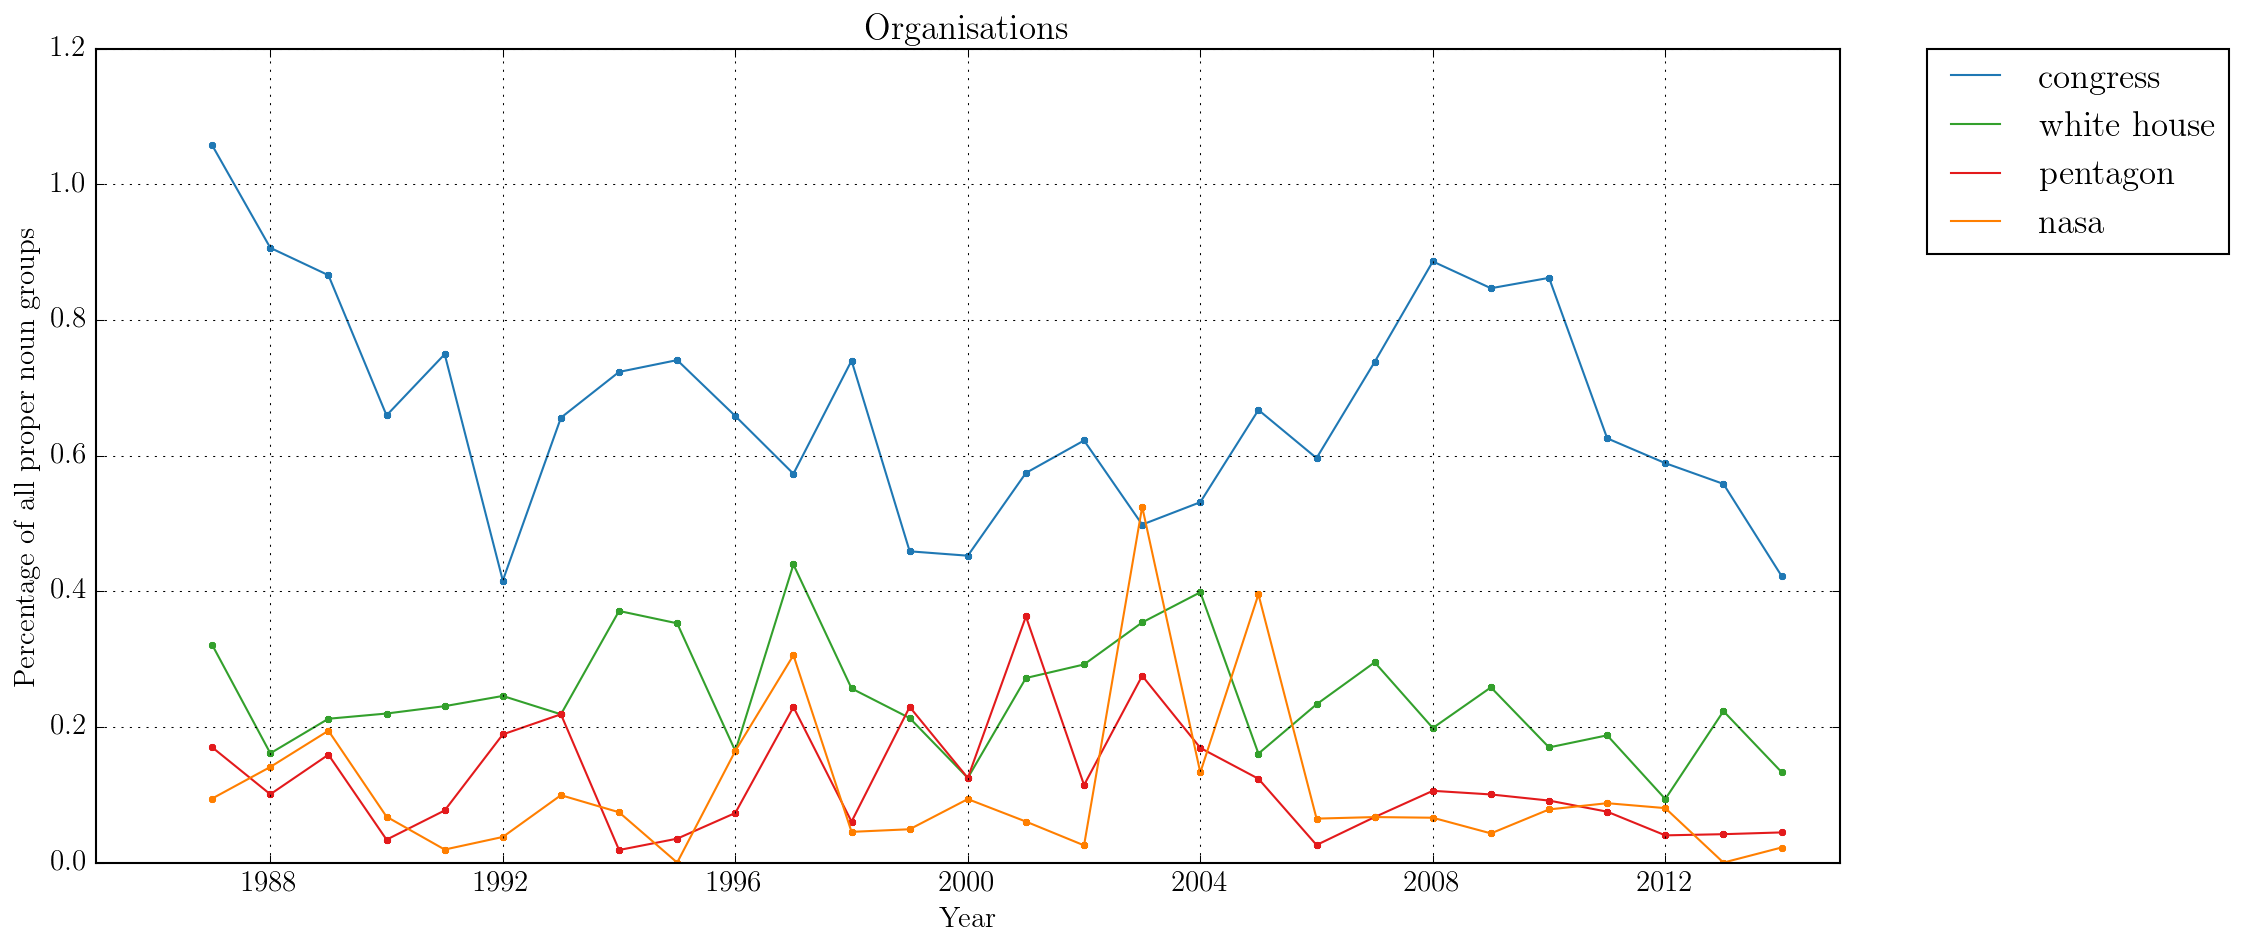
\includegraphics[width=\linewidth]{../images/organisations}
    \caption{Organisations} \label{fig:e}
    \end{subfigure}
    \begin{subfigure}{.64\textwidth}
    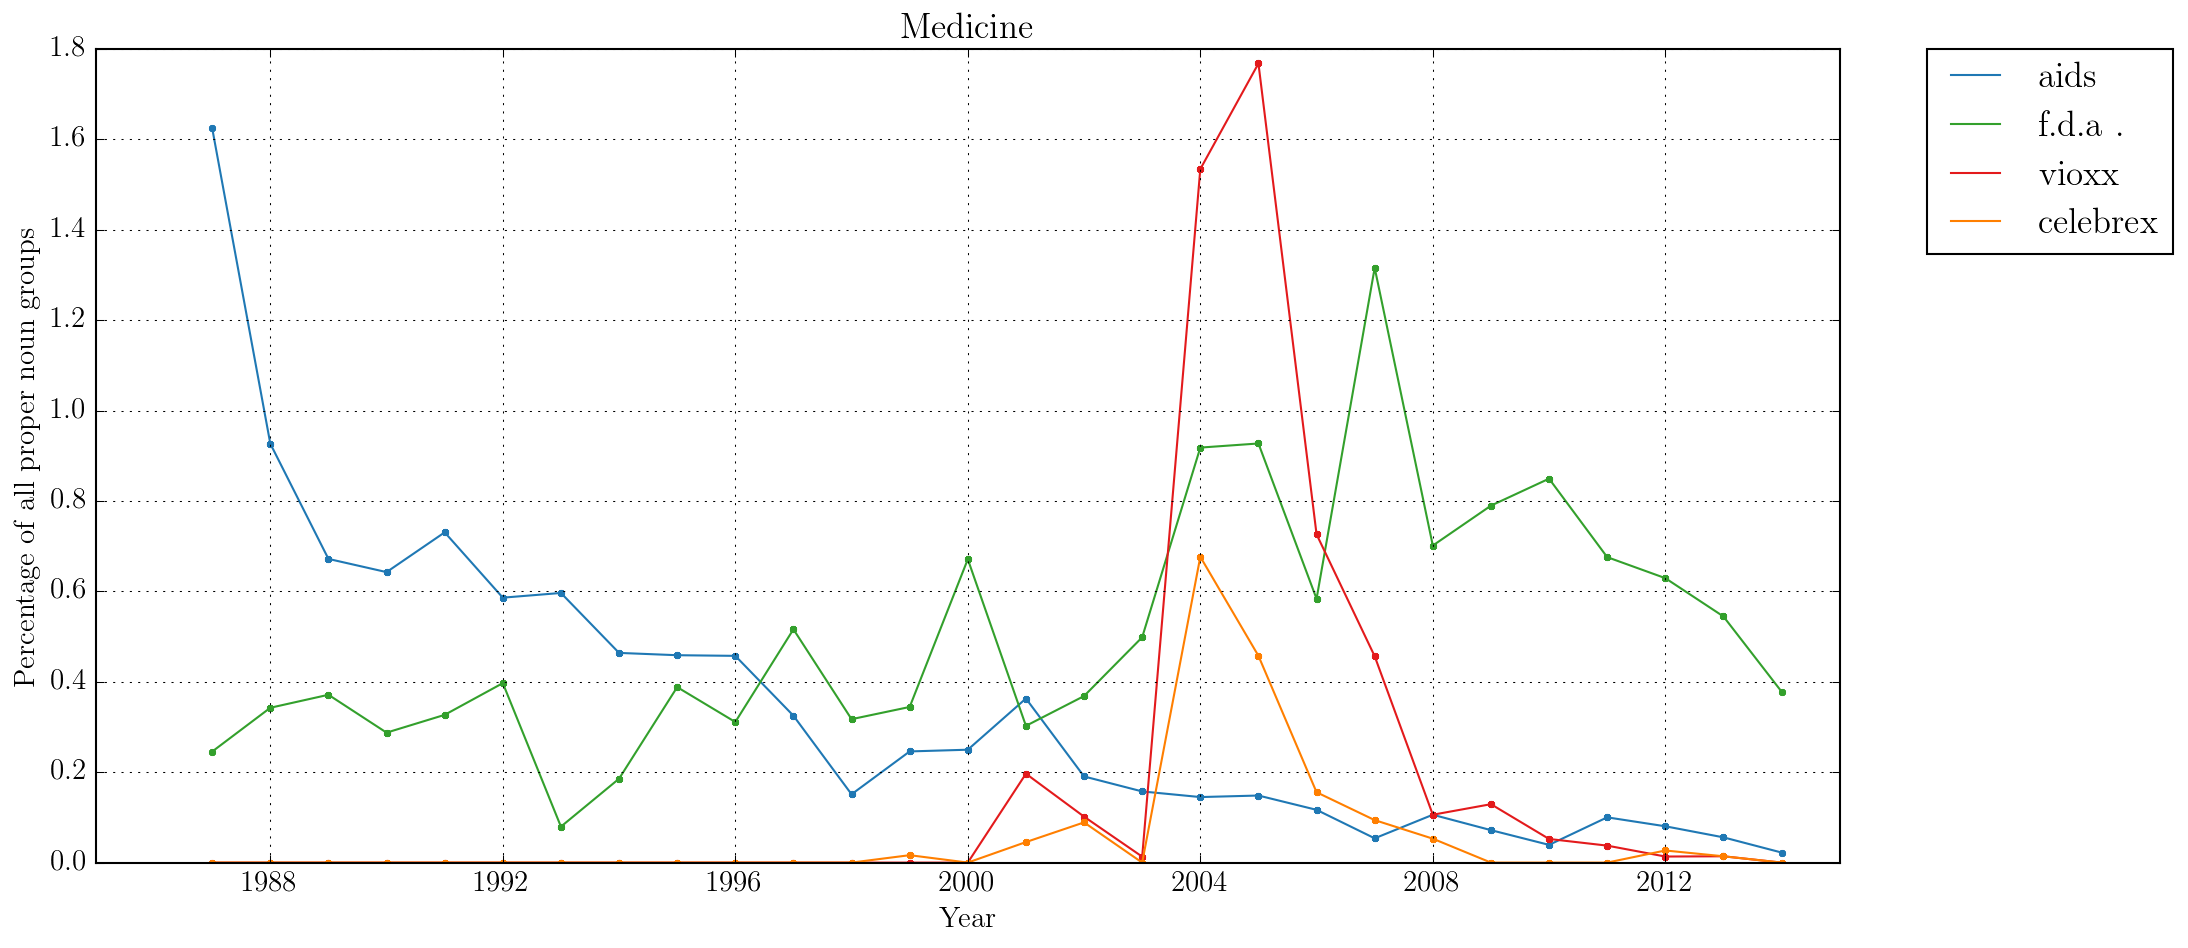
\includegraphics[width=\linewidth]{../images/medicine}
    \caption{Medical terms} \label{fig:f}
    \end{subfigure}
    \caption{Proper noun groups co-occurring with risk} \label{fig:propernouns}
    \end{figure}
    \end{landscape}

    A number of historical events were easily recognisable within the peaks and troughs of these charts. Key events represented through these interrogations include:

    \begin{enumerate} \setlength\itemsep{0em}
    \item US presidents and presidential candidates\endnote{Though the filtering out of titles and given names collapses the distinction between Bushes and Clintons, we can still reasonably infer which was being spoken about at which, and doubt can be eliminated by concordancing}~(Figure~\ref{fig:a})
    \item The First Persian Gulf War (Figure~\ref{fig:b})                   
    \item The Iraq Wars (Figure~\ref{fig:b})
    \item September 11 and the War in Afghanistan (Figure~\ref{fig:b})   
    \item The beginning of the 2014 Crimean crisis (Figure~\ref{fig:b})       
    \item The Asian financial crisis (Figure~\ref{fig:c})
    \item The breakup of the Soviet Union (Figure~\ref{fig:c})
    \item The Eurozone crisis (Figure~\ref{fig:c})
    \item The Space Shuttle Colombia Disaster (Figure~\ref{fig:d})
    \item The collapse of Enron (Figure~\ref{fig:e})
    \item The U.S. subprime mortgage crisis  (Figure~\ref{fig:e})
    \item The U.S. outbreak of HIV and the AIDS crisis (Figure~\ref{fig:f})
    \item The recall of Vioxx (Figure~\ref{fig:f})
    \end{enumerate}
    %
    This area of our investigation is by far the most promising as a means of connecting risk language to particular people and events. Spatial considerations have precluded a full treatment of the charting of risk language to specific events, despite the fact that enough data exists for detailed analyses of any number of potential foci. Future research that centres on detailed exploration of health domains (including the Vioxx recall) is planned.

    \vspace{5mm}\noindent\begin{tcolorbox}[colback=yellow!5,colframe=yellow!40!black,title=Summary: risk and proper nouns]
    \parbox{1\textwidth}{%
    We can use proper nouns to see which people, places and things co-occur with discussion of risk.}
    \end{tcolorbox}
    \vspace{5mm}

\section{Summary of key findings}

    We found that the behaviour of risk words has changed longitudinally in a number of key respects:

    \begin{enumerate}
    \item Risk words appear to be increasing in relative frequency, with modest increases in the number of unique risk words per year.
    \item Risk as a process is declining in use, and has been overtaken in frequency by risk as a participant.
    \item Risk is more often an experiential object than an experiential subject. The gap has widened considerably over time.
    \item \emph{Calculated risk} has been overtaken by \emph{potential risk} in overall frequency. \emph{High-risk} spikes in frequency in references to H5N1.
    \item When risk is a participant, quantification is often at the centre of the experiential meaning. The high proportion of mental processes highlights a portrayal of risks as perceived.
    \item Both \emph{pose risk} and \emph{put at risk} have overtaken \emph{run risk} in frequency. Use of the prototypical risk process, \emph{to risk} is declining. Finally, there is some evidence for reduced agency the \emph{run risk} process.
    \item When risk is a process, risked things\slash potential harms often pertain to individual health. This contrasts with processes as potential harm, which generally relate to people in positions of power.
    \item Common risk modifiers (\emph{risky}, \emph{riskier}, \emph{riskiest}) are gradually being displaced by a number of less common constructions (e.g. \emph{low-risk}, \emph{at-risk}, \emph{risk-averse}, \emph{risk-free})
    \item While risk as a modifier is often used in the context of finance\slash commerce, \emph{at-risk} typically attaches to vulnerable human demographics.
    \item  Longitudinally, risk words are shifting to less focal parts of clauses. We can approximate these changes using both indices or semantic function information within dependency parses.
    \item Proper nouns co-occurring with risk words highlight the close relationship between risk and health discourse.
    \end{enumerate}
    %
    As will be discussed in Chapter \ref{chap:discussion}, many of these shifts appear to be a part of a broader discourse-semantic trend of implicitness and inarguability of risk. 

    % In the following chapter, interrogations used here are applied to subcorpora of Economics, Politics and Health articles.

 % Findings: annual

%%!TEX root = ../risk_report.tex

\chapter{A comparison of economics, health, and political risks}

In this chapter, we use subcorpora of economics, health and politics articles to understand how risk words change in specific semantic fields. Due to the smaller size of these subcorpora, as a general rule, the kinds of specific grammatical queries used in the previous chapter were not useful, as they generated very low numbers of results. Accordingly, this part of our investigation includes analyses of keywords and n-grams. 

            \begin{figure}[htb!]
            \centering
            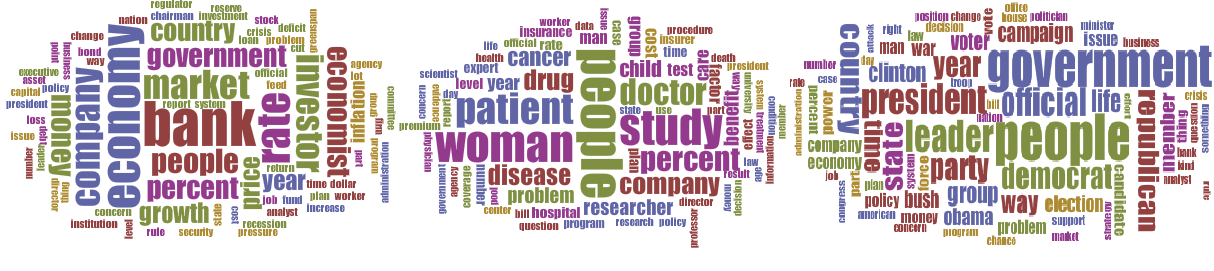
\includegraphics[width=0.70\textwidth]{../images/clouds.png}
            \caption{Key participants in the \emph{Economics}, \emph{Health} and \emph{Politics} subcorpora}
            \label{fig:clouds}
            \end{figure}

            \begin{figure}[htb!]
            \centering
            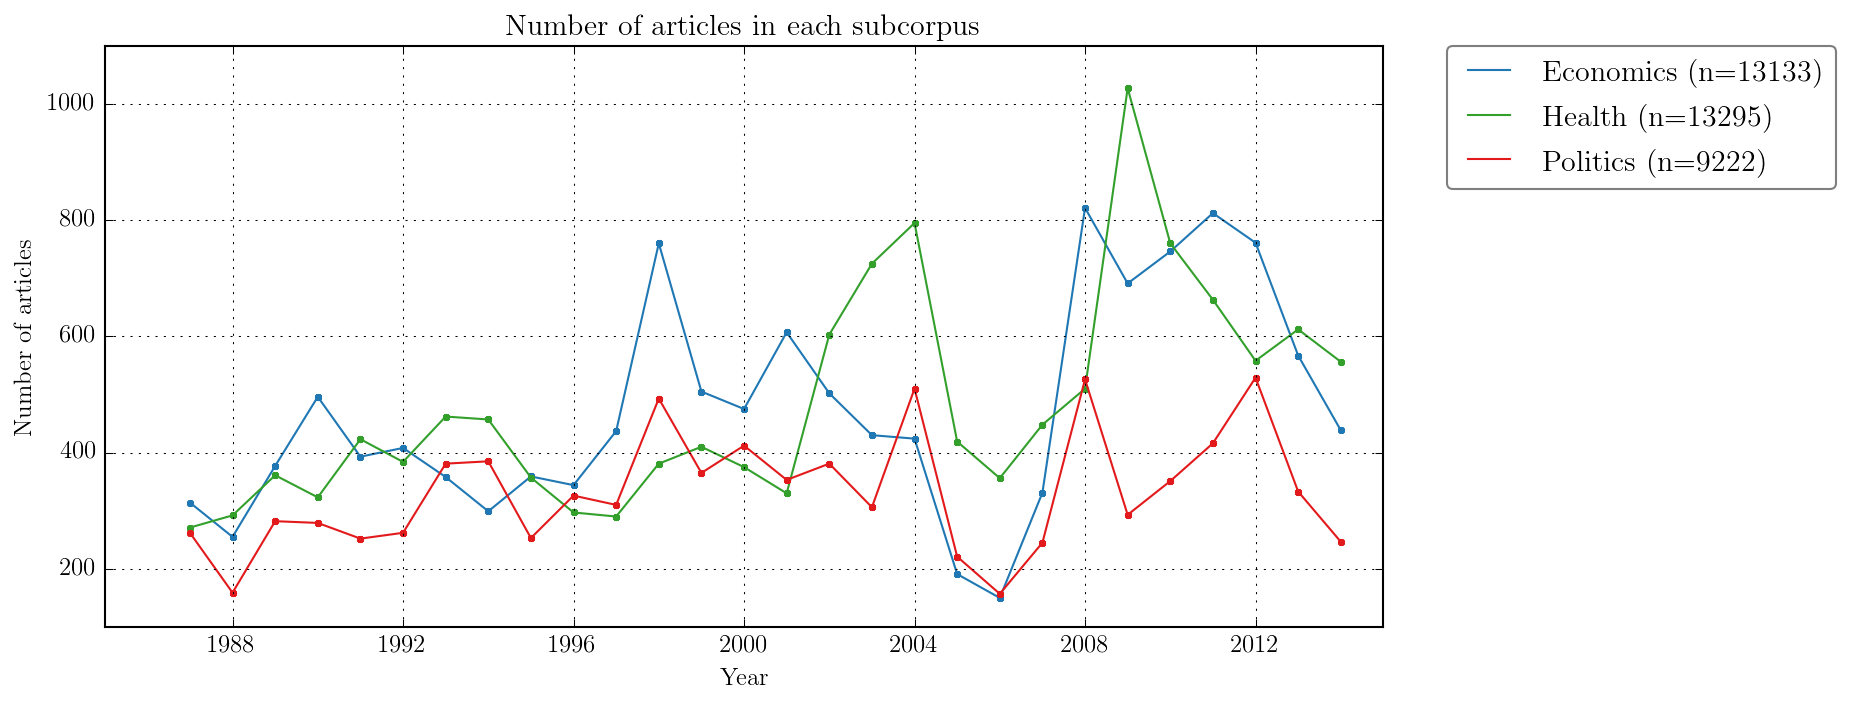
\includegraphics[width=.70\textwidth]{../images/number-of-articles-in-each-subcorpus.png}
            \caption{Number of articles in each subcorpus}
            \label{fig:article_per_subcorpus}
            \end{figure}

            \begin{figure}[htb!]
            \centering
            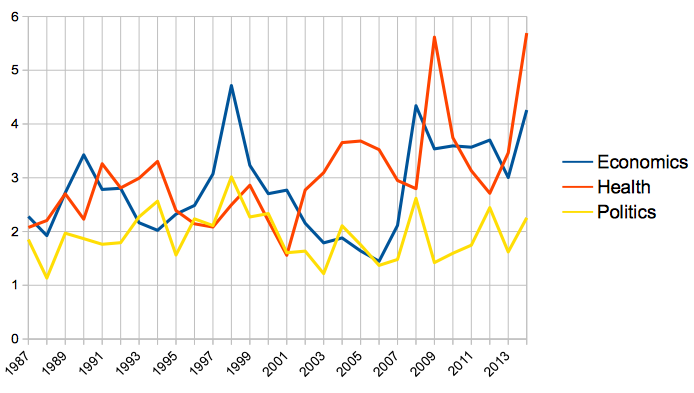
\includegraphics[width=.70\textwidth]{../images/echepol_riskwords.png}
            \caption{Risk words per total number of article topics per year}
            \label{fig:echepol_riskwords}
            \end{figure}
            %
            %Due to time constraints, we restricted the topic comparison to domains that had yielded interesting insights in the earlier interrogations. Further, we found that the smaller size of the subcorpora limited us to lexicogrammatical queries that outputted a large enough number of results for quantitative reliability. Thus, we focussed on the following three areas:

             \begin{table}[htb!]
             \centering
             \small
             \begin{tabular}{|l|l|l|}
                          \hline
                          \textbf{Economics}   & \textbf{Health}         & \textbf{Politics}     \\ \hline
                          political   & high           & political    \\ \hline
                          big         & great          & great        \\ \hline
                          economic    & low            & big          \\ \hline
                          financial   & other          & high         \\ \hline
                          great       & serious        & own          \\ \hline
                          high        & financial      & serious      \\ \hline
                          more        & potential      & new          \\ \hline
                          real        & medical        & real         \\ \hline
                          systemic    & more           & considerable \\ \hline
                          significant & significant    & more         \\ \hline
                          new         & cardiovascular & other        \\ \hline
                          little      & political      & significant  \\ \hline
                          global      & possible       & economic     \\ \hline
                          serious     & small          & financial    \\ \hline
                          other       & real           & potential    \\ \hline
                          excessive   & such           & personal     \\ \hline
                          potential   & genetic        & little       \\ \hline
                          such        & ovarian        & such         \\ \hline
                          much        & same           & public       \\ \hline
                          own         & bad            & military     \\ \hline
                          \end{tabular}
                          \caption{Most common adjectives modifying nominal risks in the topic subcorpora}
                          \label{tab:echepo_adjmod}
             \end{table}

\section{Health}

    Our topic subcorpora were much smaller than our main corpus. As a result, lexicogrammatical querying did not yield quantitatively reliable results. Accordingly, other kinds of corpus linguistic investigation, not reliant on grammatical structure, were applied. 

    First, we considered \emph{keywords}---that is, words that were unusually frequent within the health corpus when compared to the corpus as as a whole.

    Linear regression was used to determine the slope of each keyword's trajectory, and ensure that the p-value of this slope was below 0.05. Results were then sorted into two groups, based on the incline\slash decline of the slope.

    \begin{figure}[htb!]
    \centering
    \begin{minipage}{.48\textwidth}
    \centering
    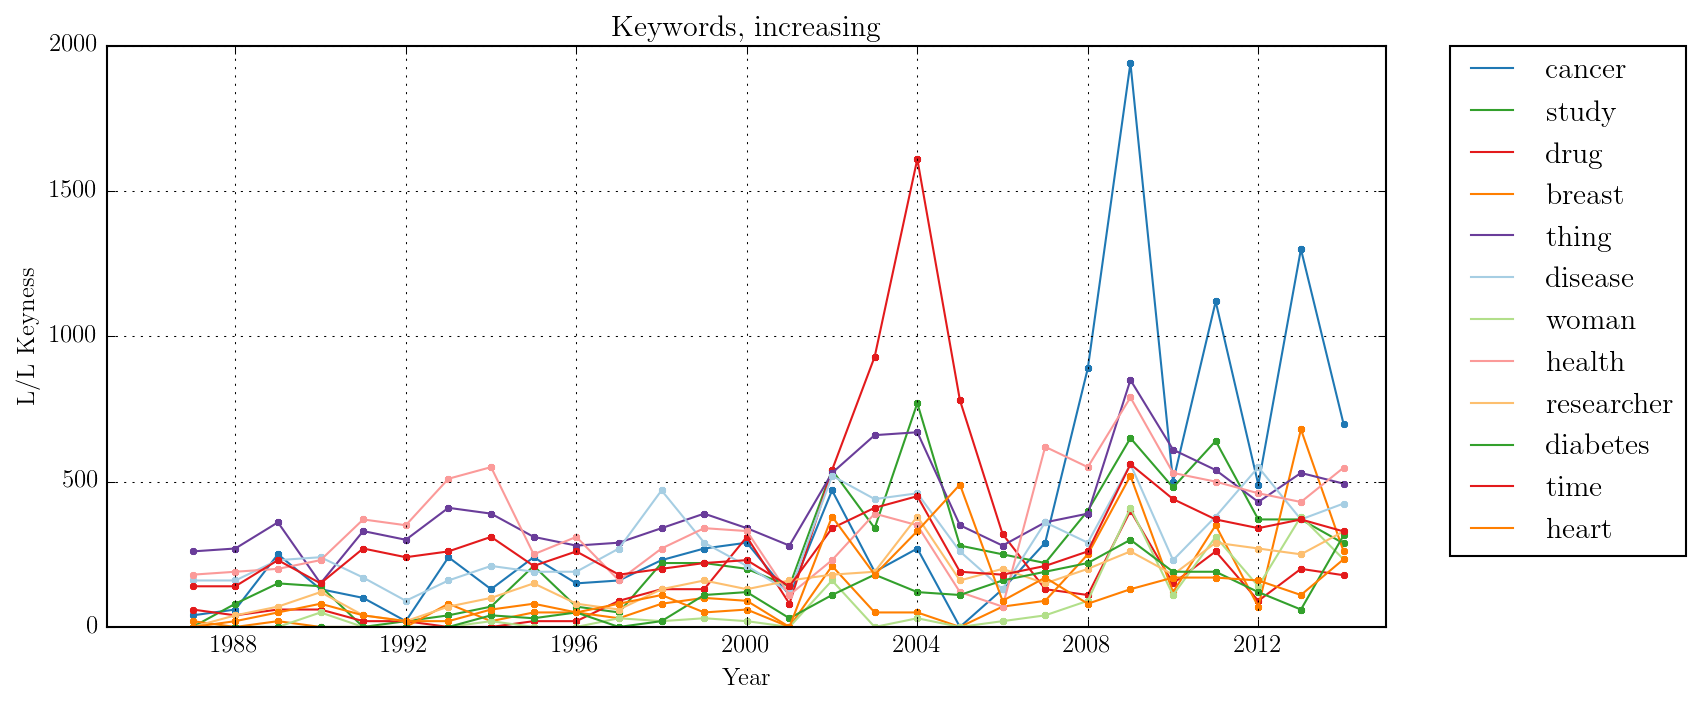
\includegraphics[width=.95\textwidth]{../images/keywords-increasing.png}
    \caption{Keywords becoming more key over time}
    \label{fig:key-inc}
    \end{minipage}%
    \begin{minipage}{.48\textwidth}
    \centering
    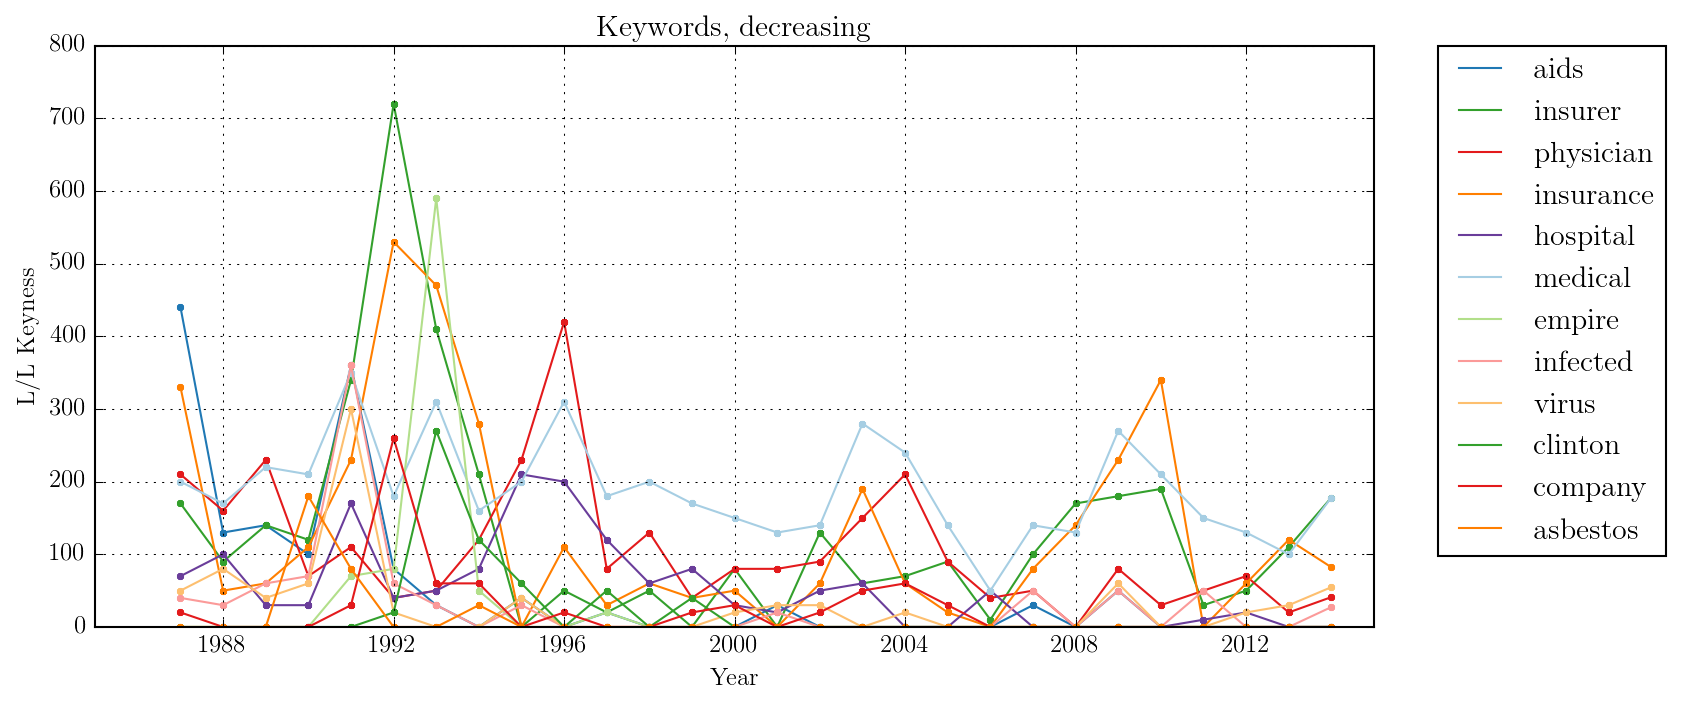
\includegraphics[width=.95\textwidth]{../images/keywords-decreasing.png}
    \caption{Keywords becoming less key over time}
    \label{fig:key-dec}
    \end{minipage}
    \end{figure}

    Next, we were interested in \emph{bigrams}---that is, words that occur beside each other multiple times within a corpus. Bigrams containing a stopword were excluded from analysis, as these results were generally common clusters of closed class words (\emph{in the}, \emph{of a}, \emph{one day}, etc.). Again, linear regression was used to group results into increasing and decreasing groups.

    \noindent
    \begin{figure}[htb!]
    \centering
    \begin{minipage}{.48\textwidth}
    \centering
    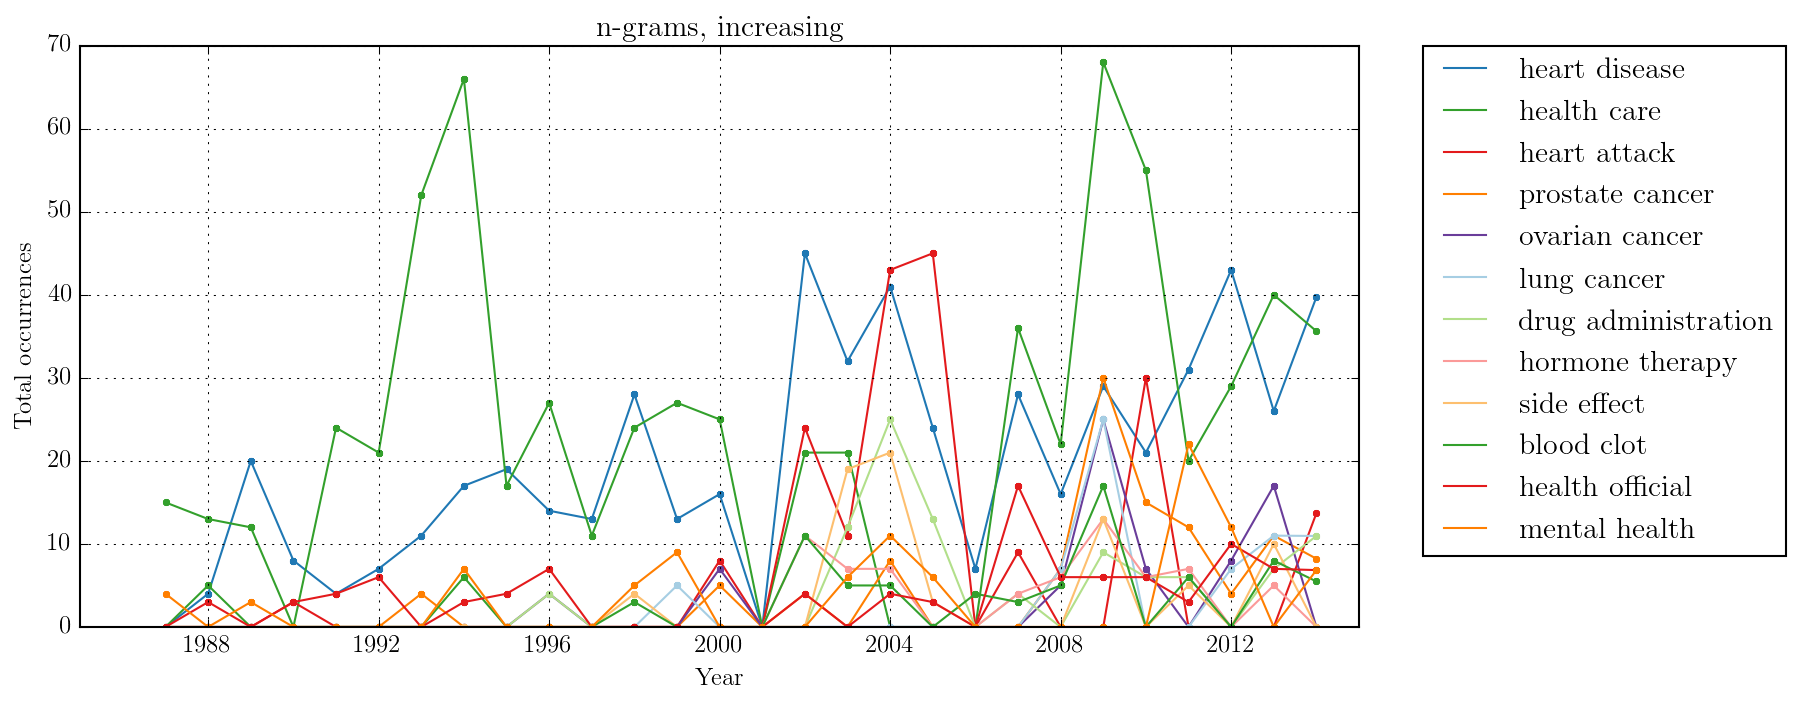
\includegraphics[width=.95\textwidth]{../images/ngrams-increasing.png}
    \caption{bi-grams becoming more frequent over time}
    \label{fig:ngram-inc}
    \end{minipage}%
    \begin{minipage}{.48\textwidth}
    \centering
    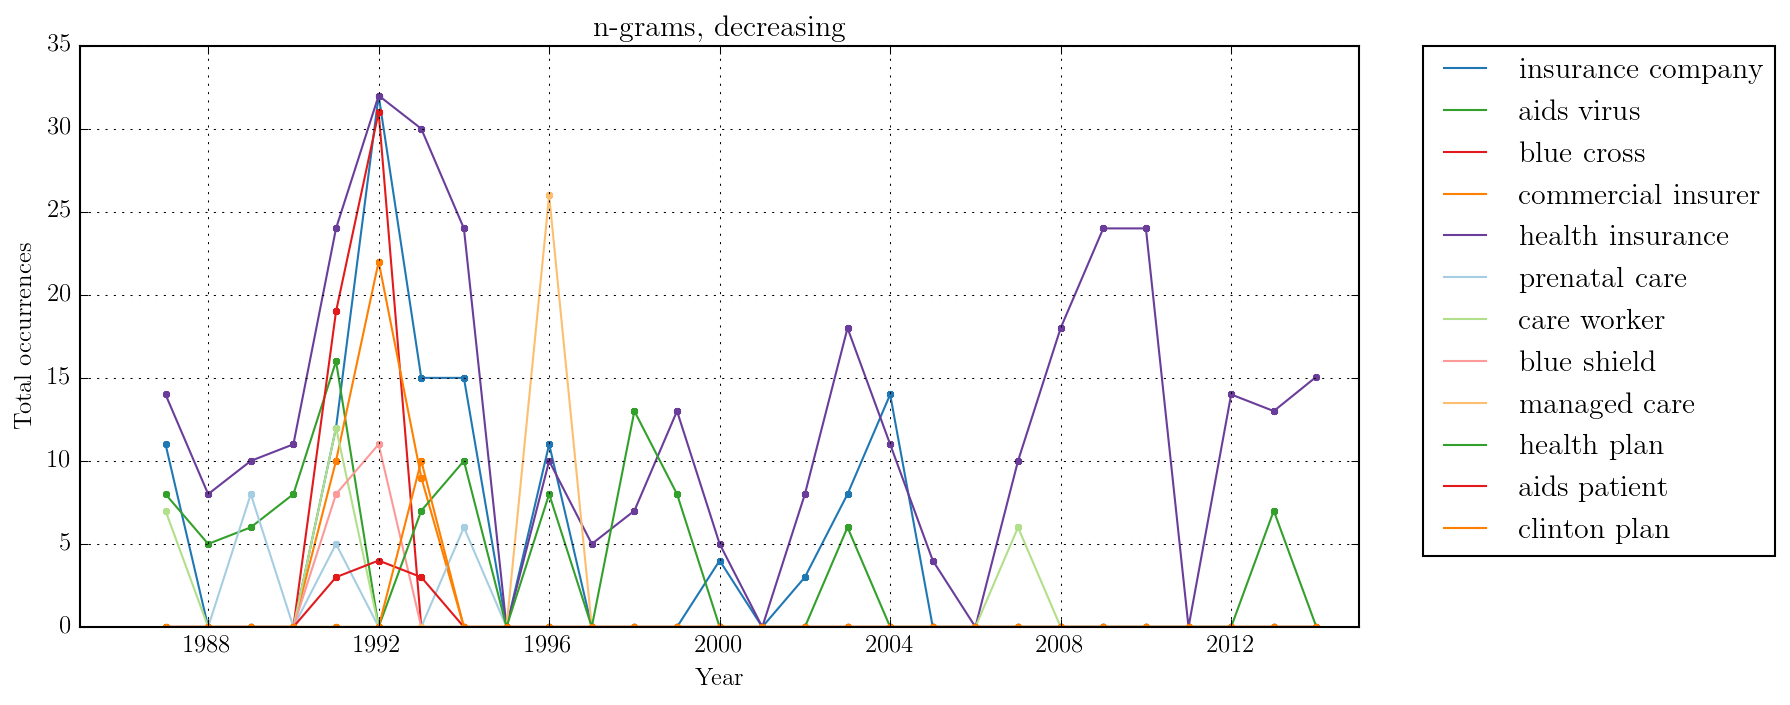
\includegraphics[width=.95\textwidth]{../images/ngrams-decreasing.png}
    \caption{bi-grams becoming less frequent over time}
    \label{fig:ngram-dec}
    \end{minipage}
    \end{figure}

We grouped these into themes, with results entered into one or more categories. Ambiguous results were often concordanced in order to determine the main context of use: \emph{athlete}, for example, could indicate the health condition (\emph{Athlete's foot}), a chain of footwear stores, or denote athletes themselves. The latter was revealed to be by far the most common context, and athlete was thus added to \emph{People, everyday}.

\subsection{Nominal groups in the health subcorpus}

The final part of our investigation of the health subcorpus looked at key nouns or nominal groups. By measuring the slope of trend lines, we could ascertain which groups were becoming more or less common.

    \noindent
    \begin{figure}[htb!]
    \centering
    \begin{minipage}{.48\textwidth}
    \centering
    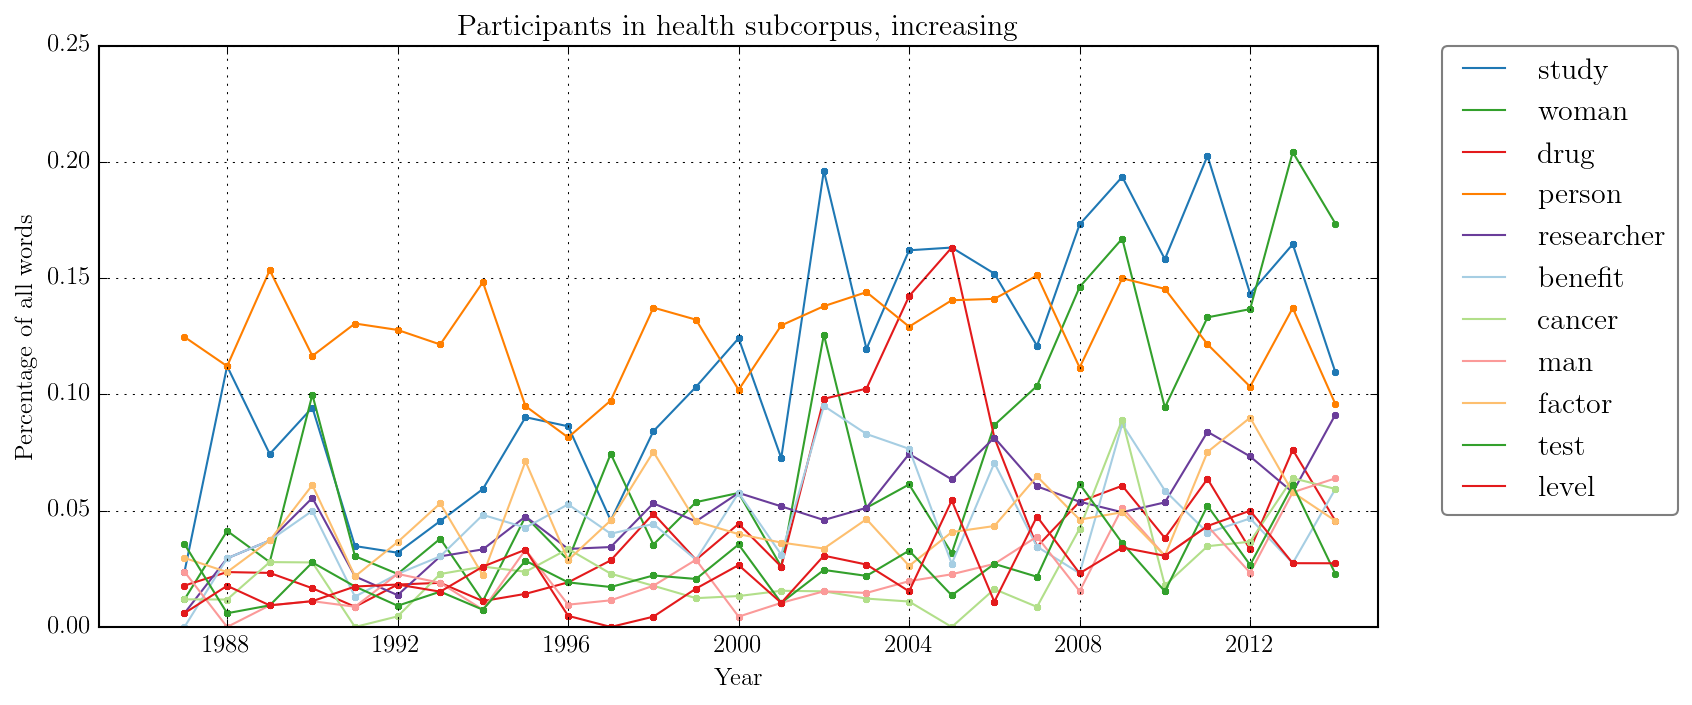
\includegraphics[width=.95\textwidth]{../images/1.png}
    \caption{Absolute frequency of nominal groups becoming more frequent over time}
    \label{fig:1}
    \end{minipage}%
    \begin{minipage}{.48\textwidth}
    \centering
    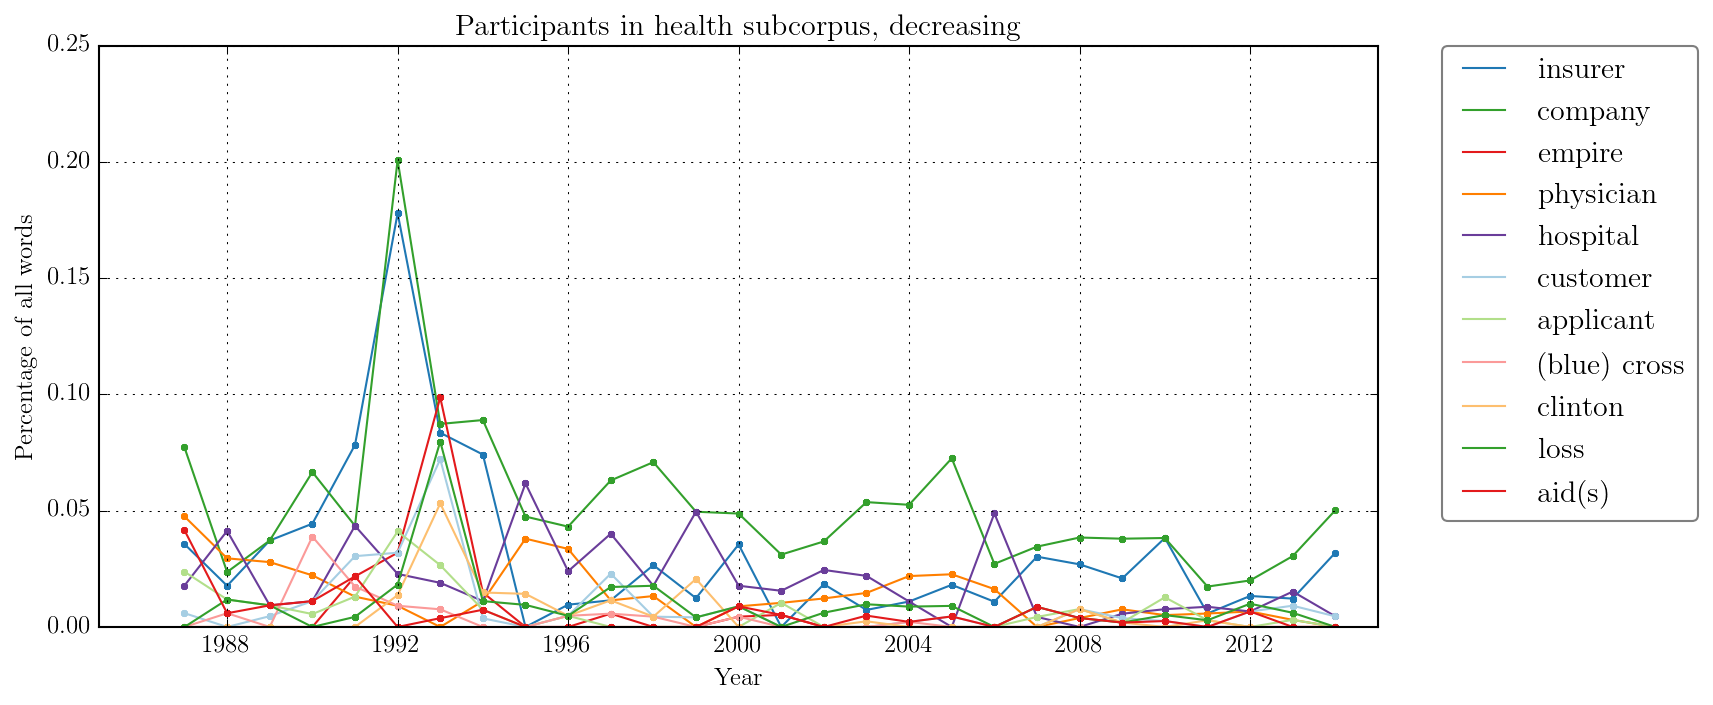
\includegraphics[width=.95\textwidth]{../images/2.png}
    \caption{Relative frequency of nominal groups becoming more frequent over time}
    \label{fig:2}
    \end{minipage}
    \end{figure}
    \noindent
    \begin{figure}[htb!]
    \centering
    \begin{minipage}{.48\textwidth}
    \centering
    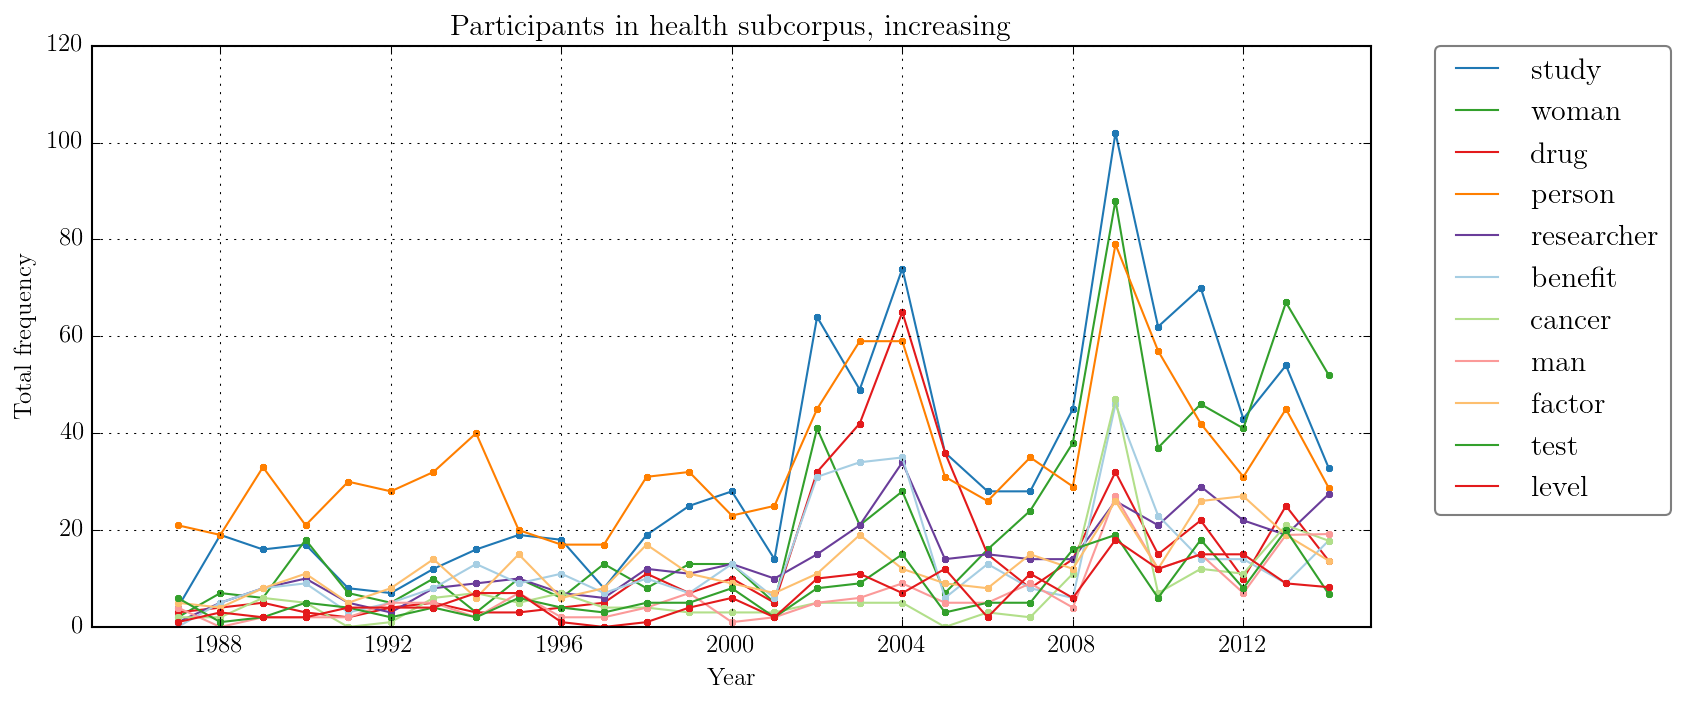
\includegraphics[width=.95\textwidth]{../images/3.png}
    \caption{Relative frequency of nominal groups becoming more frequent over time}
    \label{fig:3}
    \end{minipage}%
    \begin{minipage}{.48\textwidth}
    \centering
    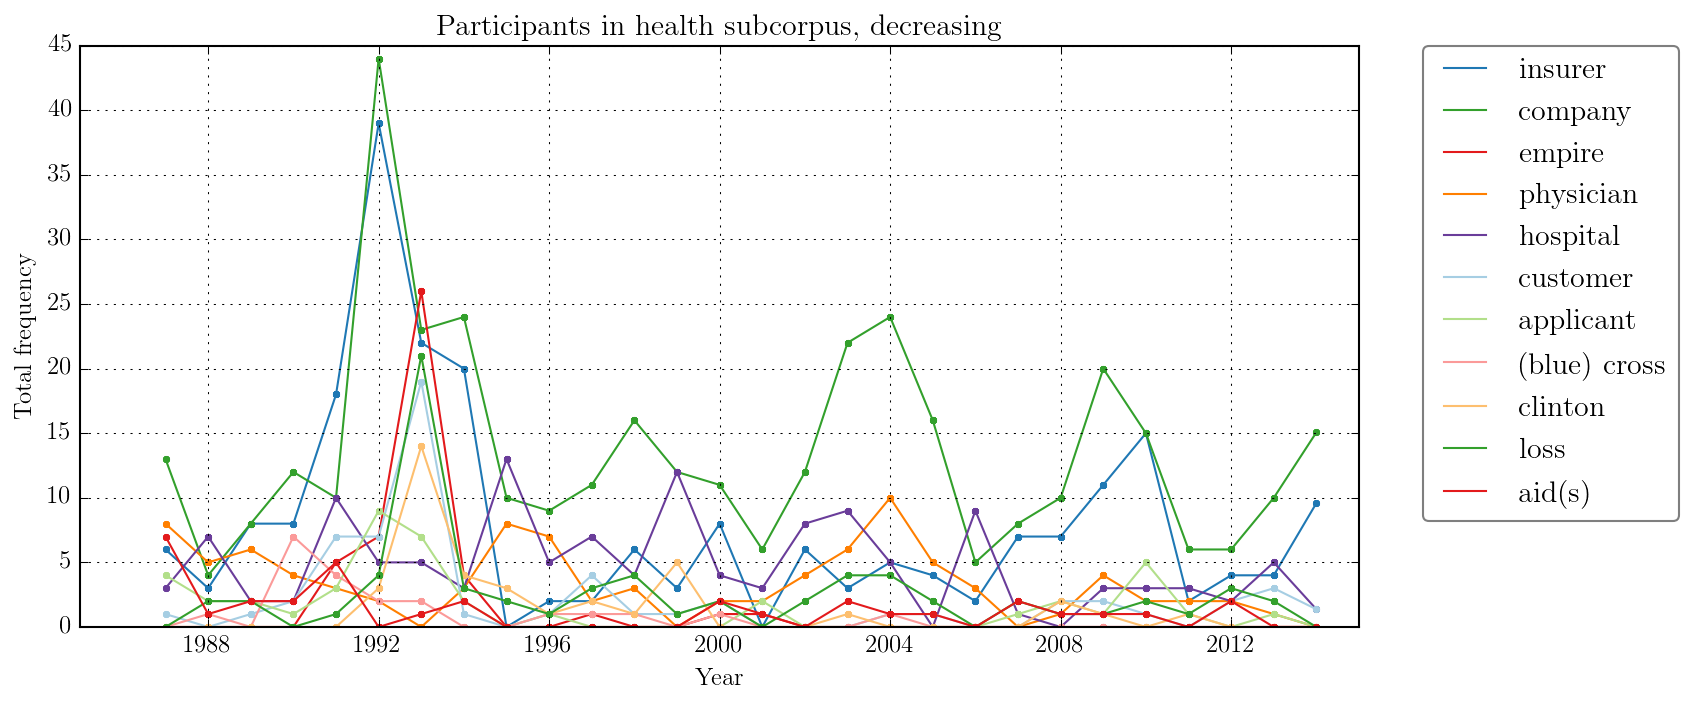
\includegraphics[width=.95\textwidth]{../images/4.png}
    \caption{Relative frequency of nominal groups becoming less frequent over time}
    \label{fig:4}
    \end{minipage}
    \end{figure}

The first major theme that emerges from this interrogation is the shift from infectious to non-infectious disease.

A second point of interest is the decline in terms related to insurance.

Though the prevalence of health insurance in mid 1990s articles was unexpected, as it corresponds with Hillary Clinton's efforts to increase health insurance coverage in the USA, unexpected was the lack of an upswing in insurance terms during the pushes for healthcare reform throughout the Obama administration.

Also apparent is an upward trend for nominal groups related to research (\emph{study, percent, research, etc.}).

This finding was of particular interest, given that the increasing contestation of academic and scientific research are core hypotheses made by Beck.

Concordancing was used to look for evidence of contestation when the nominal groups related to research were instantiated.

\section{Summary}

Broadly speaking, institutional social actors, political representatives and the like appear to have been displaced by individual human actors and components within their everyday life world.

The exception to this rule is research, which

Though further investigation into the emergence of research as a key semantic domain within risk discourse is needed, we hypothesise that it

The increasing commonality of data journalism, where journalists may conduct

Another potential factor is that the exponential increase in academic publications, as well as the increasing ease of access (via the web) has made reporting of 

This may also be a part of the increase in health risk discourse as well.

The lack of contestation points to an area in which Beck's conceptualisation of risk in late modernity may be at odds




\section{Issues in the health corpus investigation}

The first major issue was the smaller size of the corpus, which necessitated different kinds of analysis.

Within keywording and ngramming, it became clear that broader linguistic change and specific events are difficult to separate.

This, however, is where we can see the clearest examples of the link between events and language change. Interspersed throughout the keywords and n-grams are terms ranging in specificity. It is through categorisation of these varying levels that we can smooth out the 

The keywording in particular revealed a number of ambiguities. A more reliable\slash systematic method for grouping keywords would ameliorate this concern.

\section{Summary}

    The smaller size of topic subcorpora necessitated different kinds of analysis. Fortunately, such methods are well documented within corpus assisted discourse studies. Following on from these methodologies, we located particularly frequent terms, and analysed them in their context of use.

    % analysis here

    Ultimately, the ways in which a corpus can be analysed are dependent on the size of the corpus. 


%Comparing the behaviour of risk words in three smaller corpora is complicated by the lack of existing methodologies.

\afterpage{%
\begin{table}
\centering
\tiny
\begin{tabular}{|lrcl|}
\hline
1 & We know this now because                           & researchers & tested both theories , side by side , to see which \\
2 & something the public did not : Yale University     & researchers & had tentatively concluded that PPA was linked to a \\
3 & Instead ,                                          & researchers & say , young killers must be seen as extremely      \\
4 & of men with E.D. , or at risk for developing it ,  & researchers & in Italy found that the men could improve their    \\
5 & If you were an academic                            & researcher  & , you 'd have to persuade your institutional       \\
6 & Some                                               & researchers & believe hyperthymics may be at increased risk of   \\
7 & index , smoking and several other risk factors ,   & researchers & found that women on postmenopausal hormone therapy \\
8 & will have public health consequences , the         & researchers & said                                               \\
9 & Finally , and perhaps most powerfully ,            & researchers & say that a life in poverty is a life of stress     \\
10 & Office of Protection from Research Risks said the  & researchers & altered the medical records of patients , then     \\
11 & In their paper , the                               & researchers & noted that `` countries in which wine is the       \\
12 & In another study , by                              & researchers & at the University of Connecticut , leg strength    \\
13 & In an unexpected finding , the                     & researchers & reported that the women receiving goserelin also   \\
14 & that , far from protecting the heart as many       & researchers & had assumed , the therapy may have put the women   \\
15 & Now                                                & researchers & have found that elevated risk of psychiatric       \\
16 & of a New York Fire Department rescue company and a & researcher  & who is exploring the psychological bases of        \\
17 & Department of Veterans Affairs said the California & researchers & did not properly assess the safety of experimental \\
18 & Other                                              & researchers & , working with similar kinds of data , have        \\
19 & The                                                & researchers & concluded that the study '' provides the first     \\
20 & On the other hand , said Dr. Susan Czajkowski , a  & researcher  & at the National Heart , Lung and Blood Institute   \\
21 & exactly how a given AIDS patient was infected ,    & researchers & do not know exactly how much the risk of           \\
22 & In an effort to finance debts , '' the             & researchers & said , `` ordinary people are paying the ultimate  \\
23 & during the next 25 years of about 6 percent , the  & researchers & found                                              \\
24 & To obtain consent ,                                & researchers & are required to explain that the experiments are   \\
25 & slightly increasing their risks of dying earlier , & researchers & reported yesterday                                 \\
26 & Utah                                               & researchers & have videotaped 150 couples to measure the effect  \\
27 & blood cells -- became patients ' property ,        & researchers & taking them without detailed consent and explicit  \\
28 & In mapping the human genome ,                      & researchers & determined that nearly 99 percent of genetic       \\
29 & The                                                & researchers & were unable to include family history of diabetes  \\
30 & of Internal Medicine , Dr. Solomon and other       & researchers & looked at the comparative risks posed by different \\
31 & the perception of risk , said Pete Delaney , a     & researcher  & with the administration , adding that only about 9 \\
32 & The                                                & researchers & conclude that irregular sleep by itself may be a   \\
33 & Dr. Bernard H. Fox , a federal                     & researcher  & who became a pioneer in investigating the effect   \\
34 & The                                                & researchers & said it was unclear why smoking appeared to        \\
35 & The Stanford                                       & researchers & , who included Dr. Irving Weissman , a leading     \\
36 & But                                                & researchers & like Dr. Monahan and Dr. McNiel are applying       \\
37 & A study of 1,240 people by                         & researchers & at Case Western Reserve University in Cleveland    \\
38 & that of diabetes , '' said Dr. Steven G. Deeks , a & researcher  & at the University of California , San Francisco    \\
39 & In addition ,                                      & researchers & hope that the studies linking the disorder to      \\
40 & night on WNBC-TV , that Cornell University         & researchers & have found a risk of alcoholism among New York     \\
41 & , suggesting chance could play a role , but        & researchers & say the trends are credible because they are       \\
42 & The                                                & researchers & also found that patients became significantly less \\
43 & Over all ,                                         & researchers & found that calcium supplements did not lower the   \\
44 & of the power AIDS activists have mustered to push  & researchers & to do experiments that many experts deem foolish   \\
45 & The                                                & researchers & next study the extent to which medical treatment   \\
46 & was the fourth-leading risk factor for death , the & researchers & said                                               \\
47 & study 's author , Kathleen Miller , an addiction   & researcher  & at the University of Buffalo , says it suggests    \\
48 & The                                                & researchers & claim that the benefits of the research -- greater \\
49 & Some                                               & researchers & suspect genetics : Maybe thin people who develop   \\
50 & Dr. Bishop and Dr. Varmus , along with other       & researchers & , have found that the genes can cause cancer in    \\
51 & Finally ,                                          & researchers & at Tufts reported last month in The Journal of     \\
52 & The lead                                           & researcher  & , Dr. Tina V. Hartert , director of the Center for \\
53 & harmful cholesterol in the blood , even when the   & researchers & accounted for other risk factors for high          \\
54 & on cases stemming from the Sept. 11 attacks ,      & researchers & found that the more deeply therapists were         \\
55 & The                                                & researchers & did find an increased risk of other , less common  \\
56 & The inquiry in Ms. Wan 's case found that          & researchers & had adequately explained the risks to her and that \\
57 & For example , she said ,                           & researchers & are experimenting with fast-growing carp that      \\
58 & than 23,000 Greek men and women ages 20 to 86 ,    & researchers & found that napping at least three times a week for \\
59 & precision afforded by simple computing devices ,   & researchers & say , promise to deliver new insights on risk      \\
60 & only two categories of risk , minimal and great ,  & researchers & were often discouraged from doing research         \\
61 & the clear advantage of moderate drinking , the     & researchers & presented their findings with strong caveats       \\
62 & As the genes become better understood ,            & researchers & expect to find ways to block them if they become   \\
63 & adolescents followed over a period of nine years , & researchers & at the New York Psychiatric Institute found that   \\
64 & Health , for example , said that 100 psychiatric   & researchers & gathered in a room would all probably agree that   \\
65 & smoking might have damaged the fathers ' sperm ,   & researchers & said yesterday                                     \\
66 & with 20 percent of the control group , the         & researchers & found                                              \\
67 & The                                                & researchers & found that for each four-inch increase in height   \\
68 & between height and cancer may help guide           & researchers & to study hormones and growth factors that          \\
69 & Why do                                             & researchers & and willing patients test the boundaries of        \\
70 & 's disease as those who have never smoked ,        & researchers & say , and several small studies have indicated     \\
71 & But                                                & researchers & said they had never seen this before , either in   \\
72 & In 2012 , British                                  & researchers & , by combining results from clinical trials that   \\
73 & After adjusting for various health factors , the   & researchers & found that for each increase of 10 micrograms per  \\
74 & The F.D.A. has asked                               & researchers & at Columbia to reclassify the cases of self-harm   \\
75 & The                                                & researchers & said this was troubling , given recent studies     \\
76 &  A large team of                                    & researchers & , led by V. Wendy Setiawan , an assistant          \\
77 &  and violated Federal regulations because the       & researchers & had not informed patients of the risks             \\
78 &  Yet                                                & researchers & also concluded the risk of stroke was the same as  \\
79 &  In 2002 ,                                          & researchers & halted the largest clinical trial ever conducted   \\
80 &  , and while they might not be surprising to        & researchers & , they were intended to inform the public as well  \\
81 &  Many                                               & researchers & said anger-prone people could reduce the risk of   \\
82 &  Using preserved blood samples of pregnant women ,  & researchers & have found that low vitamin D levels are           \\
83 &  And so now                                         & researchers & have been working on new strategies : Developing   \\
84 &  This month , Danish                                & researchers & reported on a 15-year study of 12,000 nurses       \\
85 &  She said                                           & researchers & thought older medicine was riskier because the     \\
86 &  Last Sunday ,                                      & researchers & released data that showed that outdoor air         \\
87 &  But when the company and the                       & researcher  & are one and the same , he said , that check is     \\
88 &  Huntington 's disease and cystic fibrosis , and    & researchers & say tests identifying those at high risk of heart  \\
89 &  may increase with a father 's advancing age ,      & researchers & reported yesterday                                 \\
90 &  Denise Juliano-Bult , a                            & researcher  & at the National Institute of Mental Health , said  \\
91 &  those who gain fat around the hips and thighs ,    & researchers & say                                                \\
92 &  in the British Medical Journal in August ,         & researchers & in Argentina showed that women who were given      \\
93 &  Next ,                                             & researchers & said , they want to do a large study like one      \\
94 &  The                                                & researchers & noted that the drinks contain high levels of       \\
95 &  The                                                & researchers & offered some other examples of how the risks       \\
96 &  Some other                                         & researchers & questioned the findings , and most agreed that the \\
97 &  For purposes of comparison , the                   & researchers & also examined inherited variations in 13 genes     \\
98 &  And the flaws are compounded , the                 & researchers & said , when journalists do n't report the context  \\
99 &  A few years ago , Mercedes Carnethon , a diabetes  & researcher  & at the Feinberg School of Medicine at Northwestern \\
100 &  As with beta carotene ,                            & researchers & were shocked                                       \\
\hline
\end{tabular}
\caption{100 random instances of \emph{researcher} in the health subcorpus}
\label{tab:research}
\end{table}
\clearpage
} % economics, health, politics

%!TEX root = ../risk_report.tex

\chapter{Discourse-semantics of \emph{risk} in the NYT} \label{chap:discussion}

Accordingly to SFL, the sum total of lexicogrammar, abstracted, realises the discourse-semantics of texts. Accounting for discourse-semantic meaning involves sensitivity to realised lexicogrammatical forms, but also to the ways in which incongruence and grammatical metaphor can create similar meanings through differing grammatical constructions: as noted earlier, \emph{potential harms} may be realised as a participant in a process of risk (\emph{Bush risked losing the election}), or as a modifier of a risk participant (\emph{the cancer risk\slash the risk of cancer}).\endnote{A key issue in CADS is the ability to systematically account for rank-shifted meanings (See McDonald, Forthcoming).}~Given the diversity of roles in which risk words can appear, the delineation of risk by roles within mood and transitivity systems in the previous section was thus a methodological necessity, but one with heavy ramifications for analysis. At the level of discourse-semantics, it becomes necessary to discuss risk word behaviour more fluidly, with reference to both experiential and interpersonal meanings, and with distinctions between risk as participant, process and modifier largely collapsed. This is perhaps especially so in in our case, as risk is an example of a lexical item that may be congruently realised as either participant and process, straddling the semantic space between entity and event.

The first part of this discussion provides a description of risk in the NYT absent longitudinal considerations---something akin to the descriptions provided by \citeA{hamilton_meanings_2007} and \citeA{fillmore_toward_1992}, but from a systemic-functional, rather than frame-semantic purview. The second part is concerned with accounting for shifting discourse-semantics of risk, via the lexicogrammatical findings presented in the previous section. In the final section, longitudinal shifts are discussed in the context of specific events, broader social change, and sociological theory.

%as well as a brief commentary on the usefulness of sociological perspectives in tandem with SFL as a means of understanding the relationship between text, discourse, language and context.

\section{A monochronic description of risk}

Before turning our attention to the behaviour of risk words over time, it is useful to provide a short description of the way risk words are generally used in the NYT.

Foremost, striking is the ability of risk to function within all open word classes (noun, adjective, verb, adverb), as well as the sheer diversity of risk words. 507 unique lexical items containing risk were found\endnote{This naturally depends on your definition of a word\slash token. If we removed hyphenates or tokens containing a slash (\emph{risk\slash reward}), the list would be dramatically reduced in size. Lemmatisation would compress this list even more.}, including many (albeit vary rare) words lacking existing lexicographical description: examples such as \emph{risk-shy}, \emph{risk-addicted}, \emph{risk-elimination}, \emph{species-at-risk} and \emph{risk-happy} demonstrate the overall salience of risk and the nuance with which it is instantiated in news discourse. Further testament to this salience are the nuanced distinctions in riskers' awareness of potential harm in \emph{risking}, \emph{putting at risk, }\emph{taking} and \emph{running} risks.

        In many respects, our findings agree with those of other monochronic descriptions of risk language. First, we can see the usefulness of the frame-semantic categorisation of the kinds of participants\slash social actors that occur within the risk frame \cite<i.e.>{fillmore_toward_1992}: we often found it useful to divide corpus interrogation results into categories of \emph{risker}, \emph{potential harm}, \emph{risked thing}, and the like. Promising is the fact that in many cases, we can use the grammatical structure of the clause to automatically return lists of each kind of participant. In cases where the grammar alone cannot tell us the participant role (\emph{I risked my death}, \emph{I risked my life}), manual sorting is not difficult, as there is little ambiguity. If we insert the \emph{losing} participle (\emph{I risk losing my life}, but *\emph{I risk losing my death}), we can quickly determine if a result is a \emph{potential harm} or a \emph{risked thing}. This is especially so when risk is the \emph{process}, rather than a participant or modifier. With this in mind, focussing more exclusively on risk as process in very large parsed datasets may prove elucidating.

        Our findings also agree with a key claim made by \citeA{hamilton_meanings_2007}: health and illness risks were surprisingly prominent within our data. As will be discussed below, however, this does not appear to be a purely static phenomenon: our longitudinal analysis points toward health risks as being far more common in contemporary language than in the language of our 1963 dataset.

        A second point on which we agree is with their contention that risk words behave differently in different social situations (i.e \emph{registers}) and different genres, and that comparison of genres is worthy of further study (though here we rely on not on our dataset but on a long history of research in support of this contention within SFL):

        \begin{quote} \small \singlespacing
        We find in these discourse environments that the focus of the semantic prosody and the semantic preference changes according to the context in which they occur. While this may be something that some (but not all) sociologists of risk may have intuitively sensed in the past, there are empirical data from corpus linguistics to suggest now that the semantic prosodies can and do change slightly from one context to another \citeyear[p.~177]{hamilton_meanings_2007}.
        \end{quote}
        %
        Their dataset included transcribed spoken conversations. This register is remarkably different to that of NYT articles, and examples of risk in these contexts demonstrate this quite clearly (e.g. \emph{Don't don't risk it eh}; \emph{Cos there isn't a risk of going of there}). The key characteristics of these examples (informal lexis, unrecoverable deictic references, low lexical density, etc.) contrast starkly with our examples.

        Due to the composition of our dataset, we can have little to add to descriptions of risk in casual spoken language, aside from recognising that spoken risk talk is likely to point toward very different, and interesting, results. Though we believe our results may be generalisable to the behaviour of risk in relatively formal written contexts, extended investigation of risk in spoken corpora remains needed.

        A key finding that received little attention in this earlier linguistic research of risk language is the notion of participants' \emph{agency in risk}. Consider the following two sets of examples. The first, from 2012, shows examples of the embedded process as negative outcome.

\begin{enumerate}    [before=\itshape,font=\normalfont] \setlength\itemsep{0em} \small
        \item Some Democrats are saying the White House set itself up for the charges by making a vow that was bound to be difficult to keep and that would \textbf{risk alienating} its business supporters.
        \item Some speculated that this partnership \textbf{risked alienating} other big retailers, like 7-Eleven, by giving Starbucks influence over how Square 's payment system was developed.
        \item And campaigning on behalf of members of Congress could \textbf{risk alienating} swing voters, many of whom seem to prefer bipartisan government and dislike one-party rule.
        %\item But Cravath's pay bump will pressure competitors to increase their year-end bonuses or \textbf{risk alienating} their junior lawyers.
        %\item The changes risked alienating some parents, but ratings in certain important demographics have increased 30 percent, according to Nielsen data.
\end{enumerate}
%
The second contains grammatical subjects modified by \emph{at-risk} (from 2008):

\begin{enumerate}    [before=\itshape,font=\normalfont] \setlength\itemsep{0em} \small
    %\item Senate Democratic leaders are pushing a bill to let many at-risk homeowners do just that.
    \item He secured nearly \$100,000 for a program at the Sephardic Community Center in Brooklyn that seeks to help `at-risk immigrant youth successfully acculturate' into American society
    \item Through the years, he said, more than 1,000 at-risk young people have arrived at his doors.
    \item The document signed off on a \$1.5 million grant to World Vision, a group that hires only Christians, for salaries of staff members running a program that helps `at-risk youth' avoid gangs.
\end{enumerate}
%
Readily apparent when risk is process is that the kinds of people who risk are typically institutions or humans in positions of power and influence. Actors of risk processes are often states, politicians, or political parties. The \emph{potential harm} being risked is often an abstract concern: \emph{alienating} or \emph{offending} \emph{electorates} or \emph{allies}. In these cases, risk is a process engaged in purposively by Actors who stand to gain something equally abstract. In contrast, when risk functions as a modifier of a participant, the participant is far less powerful: women and children are at-risk of sickness; workers are at risk of injury or death. Here, risk is a quality ascribed to the self. Risky behaviour is not often mentioned. For these people, the potential harm is often recoverable from context, but not outlined within the clause. This distribution was largely consistent throughout our dataset, and will be unpacked through sociological analysis in the following chapter. % note that this may change... 

\section{Shifting discourse-semantics of risk in the NYT}

    Some lexicogrammatical and discourse-semantic phenomena have demonstrated consistent shifts over our sampling period. We turn our attention to them now.

    First, though we noted above that risk as a process involves a different set of participants to risk as a modifier, there are still longitudinal changes within this area. When looking at the \emph{risk of loss}, for example, we can see a general trend toward individual losers, rather than institutional losers. In 1963, the things at risk of loss were macro-level and abstract: athletic funding, market share, vital technology, sympathy in the west, and the like. Later, risked things are more individual assets---life and injury being the two most common. We link this conceptually to neoliberalism
    
    \subsection{Domains of risk disourse}

           \begin{figure}[htb!]
            \centering
            \addvbuffer[12pt 0pt]{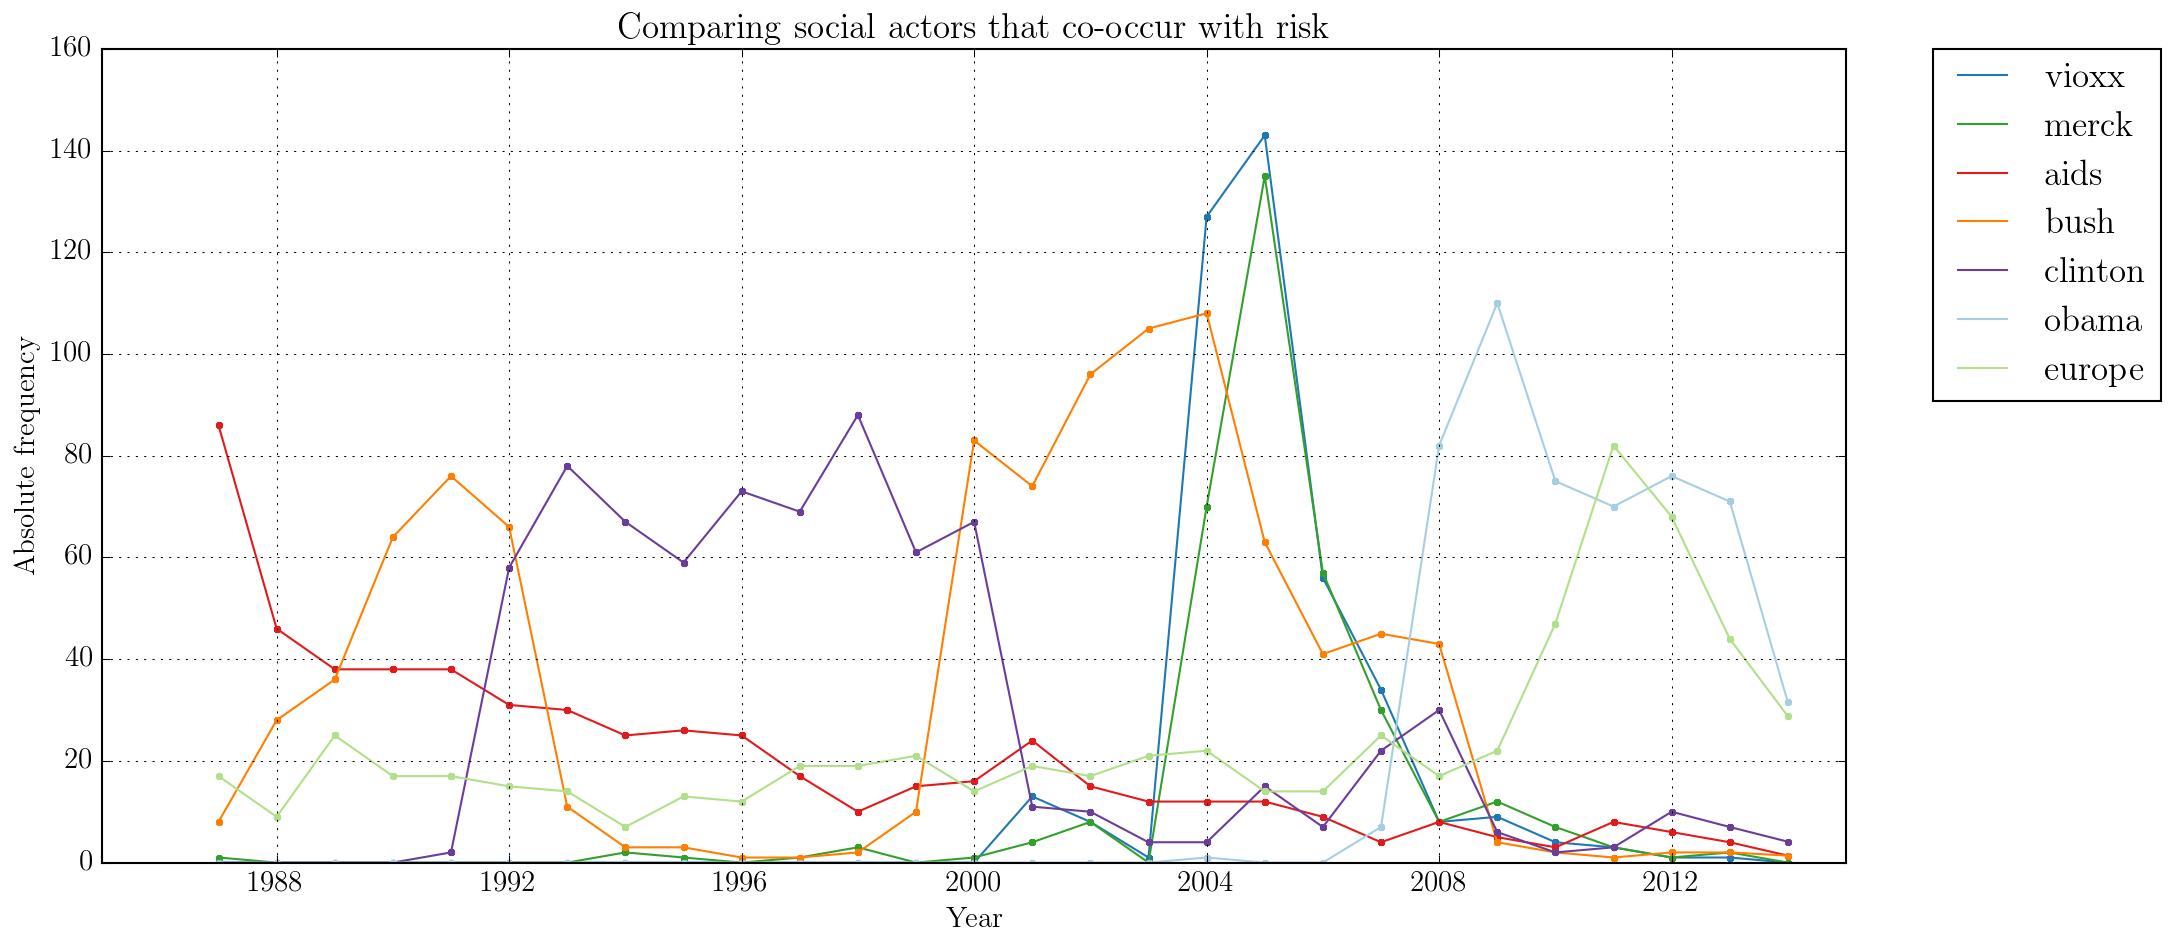
\includegraphics[width=0.75\textwidth]{../images/comparing_social_actors_that_co-occur_with_risk}}
            \caption{Comparing social actors that co-occur with risk}
            \label{fig:comparison}
            \end{figure}

        In terms of the topics in which risk words are deployed, we saw that health risks are very prominent in the more contemporary data samples. Our comparison of \emph{Risk of terror* attack} and \emph{risk of heart attack} demonstrates this preference clearly. This change is indeed a longitudinal one: in 1963 editions, a number of constructions evidence that risk was commonly instantiated with regard to diplomacy, war, international relations, and the like. In their most prominent years, AIDS, Vioxx and Merck comprise over 1.6 per cent of all proper nouns that co-occur with a risk word. This is higher than Clinton, Bush or Obama at their peaks, as well as Soviet Union in 1963\slash 1987 or Europe during the Eurozone crisis in 2011 (See Figure \ref{fig:comparison}). Moreover, in the years following the AIDS crisis, health risk have increasingly related not to infectious diseases (which require institutional responses), but to kinds of illnesses where the responsibility for prevention falls upon everyday citizens through lifestyle choices, rather than politicians, hospitals, or the FDA. Even in the case of Vioxx, where the risk was created by the premature FDA approval, risk language surrounding Vioxx remained geared toward the risks faced by everyday people. Though Merck and the FDA may be blamed, risk remains a more appropriate frame for discussing the potential for heart attack than it does for discussing the potential harm caused by improper clinical trials or financial interests causing the FDA to approve the medication prematurely\endnote{Future research will centre on unpacking the kinds of agents involved in healthcare risks of HIV, AIDS, Vioxx, etc.)}. In hundreds of co-occurrences of risk words, Vioxx and Merck, we uncovered a mere handful where the potential harm was to the manufacturer. Though we found one solid example in the 2006 subcorpus (\emph{`The verdict highlights the \textbf{risks} that Merck faces as the number of lawsuits over Vioxx continues to grow.'}), this same article containined four other risk words, each of which positions the consumer as being subject to potential negative outcomes:

        \begin{enumerate}  [before=\itshape,font=\normalfont] \setlength\itemsep{0em} \small
            \item Mr. Escobedo said that Vioxx was especially dangerous to Mr. Garza because of his other \textbf{risk} factors and that he should never have been prescribed the drug.
            \item `Mr. Garza was the last person in the world that should have been taking Vioxx,' said Mr. Escobedo, who told the jury that Merck had known since 2000 that the drug posed heart \textbf{risks} but continued selling it for four years.
            \item About 20 million Americans took Vioxx from 1999 to 2004, when Merck withdrew the drug after a clinical trial showed that it increased the \textbf{risk} of heart attacks and strokes compared with a placebo. Earlier clinical trials had also shown that Vioxx appeared to be much riskier to the heart than naproxen, an older painkiller.
            \item But recently the tide has seemed to turn abruptly against the company, as its lawyers struggle to explain a raft of documents that show its scientists were concerned about Vioxx's heart \textbf{risks} several years before Merck stopped selling the drug in 2004. 
        \end{enumerate}
     
        As \citeA{widdowson_limitations_2000} suggests, corpus linguistics often reveals things that are contrary to intuition, and this is certainly the case here. Our expectation of new risk meanings related to terrorism after 9\slash 11 was for the most part not met. Rather than a limitation, this can be treated as an insight in itself: the events and topics that come to mind when we think of risk may not necessarily correspond to the reality of risk language generally. Such is the benefit of corpus linguistic investigation of risk, when compared with previous methodologies employed within the humanities and social sciences to better understand risk.

    \subsection{Implicitness and arguability}

	   The most salient theme from the longitudinal mapping of risk is that of implicitness: increasingly common are grammatical constructions where potential harms and risked things are recoverable only from context. Below are three further examples of the \emph{at-risk} construction:

        \begin{enumerate}    [before=\itshape,font=\normalfont] \setlength\itemsep{0em} \small
            \item In 1999, we sold the company, and the next year, we moved to the United States with our two children---a third was born in 2003---so I could pursue my idea of helping low-income, \textbf{at-risk youth}.
            \item Some of the proceeds from tickets sales for the event {[}...{]} will go to support local arts programs in Washington Heights and the Broadway League's Family First Nights, which the League describes as `a nationwide program specifically designed to encourage \textbf{at-risk families} to attend theater on a regular basis.'
            \item Mr. Tepfer noted that Mr. Douglas, who was in the neighborhood when the body was found and was interviewed by the police at the time, `preyed on \textbf{at-risk women}, on prostitutes, and he engaged in sex and strangled them to death.'
        \end{enumerate}
        %  
        In these cases, what the participant is at-risk \emph{of} is not a specific negative outcome, but an interrelated set of negative outcomes that are more likely to happen to less powerful people in society. Evoked within this cluster is \emph{poverty}, \emph{drug use}, \emph{disease}, \emph{homelessness}, \emph{abuse}, \emph{fatherlessness}, \emph{dropout}, \emph{gang activity}, and the like. In many cases, \emph{at-risk} takes on a euphemistic quality, most obviously as a substitute for \emph{lower-class}, \emph{non-white} or \emph{poor}. Also interesting here is the muddying of the semantic frame: it is both difficult to determine the exact potential harm, and to classify the participant as a \emph{risker}, which seems to imply some agency or comprehension of the risk. More accurately, these participants are \emph{put at risk}---a risk process that itself is on an upward trajectory within our dataset.\endnote{Indeed, this is aligned with recent changes to the frame semantic conceptualisation of risk. At the time of writing the FrameNet entry for \emph{run risk} included the following caveat: `\emph{NOTE: This Frame is currently in the process of being changed so that some instances of at risk.n will be moved to the Being\textunderscore at\textunderscore risk frame, and some will be moved to the Risky\textunderscore situation frame. In the Being\textunderscore at\textunderscore risk frame, risk is almost always supported with at, and its external argument is the Asset}' \cite<see>{baker_berkeley_1998}.}~ 

        % https://framenet.icsi.berkeley.edu/

        This aligns with the decreasing arguability of risk. Risk in predicator or subject position is increasingly rare, as risk becomes less the nub of propositional meanings. Thus, less and less often is risk a fundamental component in meaning as exchange: in its role within complements and adjuncts, it now more typically plays a supporting role in the provision of information. A ramification of this is that risk becomes an inherent quality of participants in the field of discourse, rather than a process in which participants knowingly or by their own choice choose to engage. This shift is exemplified by the outbound trajectory of \emph{calculated risk}, and its displacement by an uncalculated \emph{potential risk}. Below are examples of \emph{calculated risk} in 1963, contrasted with \emph{potential risk} in 2008.

        \begin{enumerate}   [before=\itshape,font=\normalfont] \setlength\itemsep{0em} \small
            \item It is, of course, a \textbf{calculated risk} that Mr. Kaye is taking.
            \item Kennedy has taken a \textbf{calculated risk} here.
            \item A spokesman for the group acknowledged that granting a 10 per cent discount before a study in depth had been made was a calculated risk.
        \end{enumerate}

        \begin{enumerate}   [before=\itshape,font=\normalfont] \setlength\itemsep{0em} \small
            \item One was to make health care providers and caregivers of infected children aware of the \textbf{potential risk} of pre-chewing.
            \item At issue were the \textbf{potential risks} of having government-run funds in China and other foreign countries make big investments in American businesses.
            \item Rat pups exposed to BPA, through injection or food, showed changes in mammary and prostate tissue, suggesting a \textbf{potential cancer risk}.
        \end{enumerate}

        In the former, the existence of the risk itself has been acknowledged, and the potential harm\slash reward have been weighed. In the latter, though the situation can be identified as having potentially negative outcomes, these are formless and immeasurable. This aligns with the idea that risk (sociological reference) has come to be simply \emph{threat}.

        % It is an unspecified potentiality while calculated risk implied a degree of control.

        \subsection{Low-risk, moderate-risk, high-risk}

        \begin{enumerate} [before=\itshape,font=\normalfont] \setlength\itemsep{0em} \small
        \item Hemophiliacs, at \textbf{high risk} of AIDS, have been hard hit by the disease.
        \item Another 25 percent are \textbf{at moderate risk}.
        \item But why on this isolated campus, where no AIDS cases have been reported among students at \textbf{low risk} of catching the disease, are students so concerned?
        \end{enumerate}
            %
            During the first years of the U.S. spread of HIV, people could be classed according to low, moderate and high-risk groups. Here we have basic quantification of levels of risk. This stands in contrast to the \emph{at-risk} construction discussed above. Of these modifiers, only \emph{low-risk} emerges as an increasingly frequent form. This is also interesting, as it points to a broadening of the semantic scope of risk to include situations where risk remains present: \emph{low-resolution image} does not point toward the increased prominence of low resolution images, but more to the prominence of resolution as thing that meanings are made about. In the same way, the inward trajectory of \emph{low-risk things} does not point toward a culture of less risk, but toward a culture where even things that do not have risk are characterised by their nature to it. We could not locate existing literature supporting a claim that the salience of a concept may be evidenced not only through \emph{extreme case formulations} \emph{the riskiest, high-risk, very risky}, but through minimisation. Nonetheless, our analysis points to the idea that the increased salience of risk as a concept is in part demonstrated through its instantiation in situations where its significance is claimed to be negligible or banal.

            \subsection{Risk as modifier}

            \begin{enumerate}  [before=\itshape,font=\normalfont] \setlength\itemsep{0em} \small
                \item At JPMorgan Chase, the \textbf{risk models} hid---and were used to hide---risks from the traders and top executives.
                \item After a rogue trader cost MF Global \$141 million, Promontory came in to bolster certain areas of the firm's \textbf{risk controls}.
                \item He was a total \textbf{risk junkie}.
                \item The programs are all based on the concept of risk management, rather than the unattainable goal of total \textbf{risk elimination}.
            \end{enumerate}

            Risk occurs within many different modifier positions (see Table \ref{tab:modriskwords}). Of these, pre-head nominal types are rising, and adjectival pre-head types are falling. From these shifts, we can surmise some sociological insight related to arguability (as conceptualised by SFL). In the increasing frequency of pre-head nominal modifiers (\emph{risk management, risk arbitage, risk factor, risk insurance}---more examples above), we can see increased social significance of risk as a concept through the evolution of specific jobs whose central concern is risk (see Section \ref{sect:riskmod} for discussion of the emergence of \emph{risk factor} in particular). Pre-head nominal modification reflects the codification of a concept: such constructions must be culturally recognised constellations of meaning. In comparison, adjectives attach to head nouns relatively freely in English. Cultural recognition of the adjective-noun combination (\emph{a risky move}, \emph{the riskiest option}) is not a prerequisite for meaning to be understood.

            \subsection{Arguability} \label{sect:arg}

            Longitudinal change in the arguability of risk words is consistent. In earlier editions, risk words more commonly occupy more arguable roles, according to systemic functional grammar. In later editions, risk more commonly occurs in heavily dependent positions. Less often does a risk word form the central component being discussed; more often, it exists as a modifier of one of these components, or as a part of a supporting, subordinate clause.

            Increasing nominalisation and `participantification' of risk (See Figures \ref{fig:wordclasses} \& \ref{fig:funcrole}) are also indicative of decreased arguability. The key affordance of nominalisation is that it reduces the need to make meanings through constellations of Participants and Processes: instead, 



            Given that Processes in the Transitivity system pattern with the Finite\slash Predicator in the Mood system, nominalisation facilitates clauses with larger amounts of less arguable information.

            The discursive function(s) of nominalisation are well-acknowledged both within SFL and outside of it.

            `The interpersonal price of decreasing negotiability' (Halliday \& Martin, 1993, p.~41)

            Nominalizing `allows the writer to give the required flavor of objectivity to his or her statements and claims' (Holes, 1995: p. 260). 
            Nominalization disengages the speaker/writer from commitment to the truth of his/her statements by allowing him/her to make `unattributable claims' (Quirk et al, 1985: p. 1289);
            Nominalization has the capacity to blur/mystify agency, thus `masking real intentions' (Hatim, 1997: p. 114);

            Hatim, B. (1997). Communication across cultures. Translation theory and contrastive text linguistics. Exeter: University of Exeter Press.
            Hatim, B.  \& I. Mason (1997). The translator as communicator. London and New York: Routledge.
            Holes, C. (1995). Modern Arabic: Structures, functions and varieties. London/New York: Longman.
            Quirk, R., S. Greenbaum, G. Leech \& J. Svartvik (1985). A comprehensive grammar of the English language. London: Longman Group Ltd. 
            Stubbs, M. (1998). Language and the mediation of experience: Linguistic representation and cognitive orientation. In F. Coulmas (Ed.), The handbook of sociolinguistics (pp. 358-373). Oxford: Blackwell. 







            We are limited in our ability to interpret this result. Little has been written about the relationship between dependency grammars and SFL. As dependencies are inherently functional-semantic, rather than generative-grammatical, dependency is perhaps the most useful \endnote{Current systems for automatic systemic functional annotation tend to rely on dependencies generated with Stanford CoreNLP} mainstream grammar for learning about the semantic behaviour of a given word. That said, though functional categories provided by Stanford CoreNLP's dependency parser overlap in many respects with categories in the Mood system of SFL, there are still mismatches, or shortcomings. Most critically, dependency grammar conflates interpersonal, experiential and textual systems, while SFL demands three separate parses. As discussed earlier, the systemic-functional conceptualisation of subjecthood is threefold, whereas CoreNLP simply nominates the interpersonal subject.

            Due to the availability of nuanced querying languages for phrase structure grammar annotation, our investigation leaned toward grammatical structure annotation over dependency grammar. This is despite a problematic relationship between functional and phrase structure grammars. Given that interesting preliminary findings were unearthed by querying dependency information, we conclude that further exploitation of dependency annotation for the purpose of risk language analysis appears to be a promising area for further analysis.

	\section{Sociological perspectives}
            
	The task that remains is to connect observed shifts to their temporal context. In terms of the annual subcorpora, this was by no means a clear-cut task.

	When focussing on the subcorpora of economic, health and political risks, linguistic reactions to real-world events were much easier to locate. We concluded that further investigation of risk would do well to focus on risk as instantiated within texts sharing a semantic field. 

            Our investigation of topic subcorpora was limited by scope. That said, the open-source tools we have developed for interrogating corpora for discourse analysis could easily be put to use in an investigation of a topic subcorpus.

	%~\ \todo[inline,color=green!40]{\noindent Mapping events to risk instantiation in the topic subcorpora here}
	
	We found little evidence that health crises resulted in increased frequency of risk in articles centred on economics or politics. This seems to suggest that while real-world events influence the instantiation of the risk semantic, this instantiation remains more or less limited to the field(s) of discourse to which the real-world event is most related.

	A final point of interest is that adjectival risk words in some respects behaved contrary to our expectations. Simple adjectival risks as modifiers of participants (\emph{the risky manoeuvre}, \emph{riskier choices}) appear to be decreasing in frequency. Furthermore, though there is a very large variety of adjectival risks, and though there is a general trend toward a greater number of risk adjectives, this increase is a slight and gradual one.

	Perhaps in this finding there is some evidence for the Risk Society thesis, in that the ways in which risk can characterise a situation were more or fully articulated during high modernity. Though these characterisations continued to be applied today, saturation point may have been reached.

    %\emph{What can be concluded from the finding that real world events do not appear to have long-lasting effects on the behaviour of risk words?}

    %Ultimately, perhaps we should not be surprised by this finding. Language is a system that must be resilient against such influences: if single events caused meaningful changes in the lexicogrammatical behaviour of a single word, communication between those aware of and unaware of events would be made more difficult. Accordingly, our suggestion would be that temporary change in the behaviour of a word (as can be seen in spikes in the number of risk words surrounding certain events) are interesting in and of themselves. Moreover, these changes can potentially be measured in pseudo-real-time by mining RSS feeds, using the Twitter API, and so on. Lexicographers could take note of which kinds of events bring about instantiation of a certain word or concept, and create definitions accordingly. Discourse analysts and sociologists could hypothesise the co-occurrence of certain kinds of language with certain kinds of events, and use real-time data to confirm or refute these hypotheses. Cooperative efforts between functional linguistics and sociology, however, are dependent upon a reconciliation of divergent conceptualisations of the relationship between text and context. This issue is elaborated below.

 % discourse semantics in NYT

%!TEX root = ../risk_report.tex

\chapter{Limitations of the study}

	Our methodology was innovative, and involved fitting theories, practices and tools together in novel ways. Through the course of our investigation we noted two major clusters of limitations. The first were issues relating to the performance and epistemological consequences of digital tools used during the investigation. In short, available digital tools may not perform as desired. In the case of parsers, this is generally an incorrect parse. 

	%	%\noindent Also an issue is that Stanford CoreNLP uses phrase structure and dependency grammars, rather than SFG (for which fewer computational resources are presently available). We were thus left with the task of translating systemic ideas into phrase structure grammar and dependency grammar. This process was often time-consuming and counter-intuitive, as well as theoretically difficult to reconcile. In the case of topic modelling, rather than erroneous, results may simply be unhelpful. The modeller is blind to grammatical structure as well as the division of language into three metafunctions. Accordingly, MALLET groups texts based on words that are unlikely to contribute not contribute to the semantic field of the text (\emph{like, please, to, having, could}). Furthermore, MALLET's conceptualisation of topic may differ markedly from a human reader's: in one iteration of the topic modelling, MALLET grouped together articles about African American religious issues and chess, apparently based on the co-occurrence of words like \emph{black}, \emph{white}, \emph{saving} and \emph{bishop}.

	The second major issue unearthed during the investigation concerned the size of the dataset, which, aside from being simply computationally intensive, was also so large that it constrained the kinds of analytical methods available to us. With 29 annual subcorpora, as well as three topic subcorpora, we struggled to simultaneously maintain a focus on minute changes in lexicogrammar and to connect change generally to events of interest to sociologists. Indeed, though instantiations of risk words may react to current events, further subdivision of the corpus into weekly/monthly subcorpora proved too unwieldy. A similar investigation could be carried out on one subcorpus alone, divided into weeks or months, in order to better assess the influence of individual events. The richness of the data also prevented direct comparison of more risk fields, with only a cursory treatment of government and health risks given here. A final issue caused by issues of data size was that we were unable to manually check each

	 Search query output was manually read to determine that the correct features were being located. What was missing as a result of parsing problems or query design likely went unnoticed amongst the streams of text. By the conclusion of the interrogation, millions of clauses had been manipulated, millions of features extracted and counted---mistakes are unfortunately bound to remain.

\section{The limits of lexicogrammatical querying}

        A major issue we face, and have not dealt with head-on, is the potential for similar discourse-semantic meanings to be made via a number of different kinds of lexicogrammatical arrangements:

        \begin{enumerate} [before=\itshape,font=\normalfont] \setlength\itemsep{0em} \small
            \item Risked money was lost
            \item They risked their money
            \item They risked their savings
            \item Money was risked
            \item The money, which they risked, was lost.
            \item They had money. They risked it.
        \end{enumerate}

        Each of these hypothetical examples communicates that money was risked, but through different grammatical strategies, ranging from the group level (Ex. 1) to the clause-complex (Ex. 6). With great difficulty, we could construct a query that matches every one of these results, or merge the results of a number of searches. As the queries grow in complexity, however, undesirably results may creep in: a query matching \emph{money} in the above cases would also likely match \emph{death} in \emph{They risked death}, despite the fact that one is the risked object and one is the potential harm. Determining the proper functional role is simple for human coders, but the number of results in need of categorisation is often far from trivial. 

        %Furthermore, in Examples 5 and 6 (in which meanings are made across clauses) are at the very limits of even the most sophisticated kinds of grammatical and semantic annotation tools available today.

        The second major issue is the converse: counted in many our automatic queries are many examples in which the money was never risked:

        \begin{enumerate} [before=\itshape,font=\normalfont] \setlength\itemsep{0em} \small
            \item They would have risked their money
            \item They didn't risk their money
            \item Risking money was a terrible idea, so they didn't do it.
            \item Don't risk their money.
        \end{enumerate}

        Few corpus-based studies of discourse have attempted to distinguish between these kinds of meanings automatically. Though many grammars account for the notions of \emph{possibility}, \emph{counterfactuality} or \emph{negation} presented above, how to use these meanings to include\slash exclude matches has yet to be determined.

        It must also be noted, of course, that any study of text corpora necessarily involves removing text from the actuality in which it was produced. Though we can be attuned to the nature of written news journalism, we have not been able to account for meanings made multimodally (through adjacent images, advertisements, etc.). Though perhaps not a critical issue in studies of news corpora, it is nontheless important to acknowledge that in some sense we have been studying \emph{text}, rather than \emph{texts}. Synthesis of corpus findings with in-depth analyses of individual articles, or of the influence of the media production process, would no doubt improve our ability to generalise our results. Indeed, future research incorporating these perspectives is planned.

        % Predictive applications of Big Data/corpus linguistic methods have already been discussed: \citeA{michel_quantitative_2011} and \citeA{leetaru_culturomics_2011} argue that nuanced mining of large quantities of language can potentially predict civil uprisings such as those seen in the Arab Spring, for example. It must be remembered that these studies have been criticised for their far-reaching conclusions \cite<e.g.>{zimmer_when_????}, and of course that predictive applications of corpus linguistics to date have had the benefit of hindsight. Interpreting peaks and troughs in particular kinds of language is also far from straightforward: increasing numbers of risk words before 9\slash 11 could be interpreted as either a possible predictor of the event or as evidence that the event did not itself cause an increase in the use of risk words. As such, we remain cautiously optimistic about predictive applications. More practically, it seems that such applications are feasible only when there is little delay between text production and text analysis: automated analysis of language circulated via the Web seems a much more sensible starting point for predictive work than static corpora of digitised newspapers and books.


\section{Conclusions}

    Instantiation of risk words is linked to real-world events: the beginnings of the AIDS epidemic are accompanied by a spike in health risk discourse; 9\slash 11 appears to be a catalyst for increasing discussion of risks and threats of terror and war. It remains very difficult, however, to fully disentangle the constructive-responsive relationship between real-world events and instantiation of particular concepts in language. Broader ideologies and social movements may indeed be more reliable predictors of linguistic change.

    \begin{itemize}
    \item We found that it is very difficult to pinpoint the effect of individual events on risk word usage in the NYT as a whole.
        \item Our interrogation of economics, health and politics articles turned up clearer evidence of the effect of real events.
        \item Even so, our approach to the creation of the subcorpora was simple, and the topics were very broad. Manually selection of automatically located articles for more specific topics would likely result in clearer indications of the effects of events on risk word usage.
        \item The main thrust of our approach was to investigate the sum total of NYT articles during the sampling years.
        \item While political risks peaked during US election times, this could not be observed when analysing the corpus as a whole.
        \item Accordingly, our findings pointed more toward the influence of broader social movements than to specific events.
        \item We interpreted many of the changes in the behaviour of risk words as evidence for \textbf{neoliberalism} and \textbf{reflexive modernity}.
        \item Indeed, the corpus developed for this study could be reused in a multitude of ways to 
        \item Finally, it must be borne in mind that the NYT is merely one newspaper, and newspapers are merely one genre
        \item We selected NYT for its size, consistency, the availability of digitised content, and its influence in global discourse.
        \item Most obviously, the emergence of the Web challenges this set of criteria in a number of ways. Popular social networks, as well as the public web, produce exponentially more content than a single newspaper.
        \item Mining global news or blog posts via RSS feeds, or Tweets via the Twitter API, allows the quantitative analysis of voices typically marginalised or absent within mainstream media.
    \end{itemize}
    
%\bibliography{../../references/libwin} % Limitations

% %!TEX root = ../risk_book.tex

\chapter{Conclusions}

	Our project has 

	The novel methodology may prove useful to researchers interested in discourse and sociology...




\section{A research agenda for risk discourse research}









	\subsection{More areas of interest}	

	Perhaps the major limitation is on focussing only on risk words to the exclusion of potential

	While necessary here for reasons of scope, the results are indeed 

	\emph{Danger}, \emph{threat}, and \emph{insecurity}. These terms likely 

	Future corpus-based exploration of discourse-semantic change could use methods to map out the behaviour of related concepts, as well as their interrelationships.

\section{Conclusion}

	Of course, instantiation of risk words is linked to real-world events: the beginnings of the AIDS epidemic are accompanied by a spike in health risk discourse; 9\slash 11 appears to be a catalyst for increasing discussion of risks and threats of terror and war. It remains very difficult, however, to fully disentangle the constructive-responsive relationship between real-world events and instantiation of particular concepts in language. Broader ideologies and social movements may indeed be more reliable predictors of linguistic change.

	



%\bibliography{../../references/libwin} % research agenda, conclusions

%end matter

	\cleardoublepage
	\singlespacing
	%\footnotesize
	\printendnotes
	\cleardoublepage
	\singlespacing
	\bibliographystyle{apacite}
	\bibliography{references/refs}
	\cleardoublepage

	\end{document}
